% Options for packages loaded elsewhere
% Options for packages loaded elsewhere
\PassOptionsToPackage{unicode}{hyperref}
\PassOptionsToPackage{hyphens}{url}
\PassOptionsToPackage{dvipsnames,svgnames,x11names}{xcolor}
%
\documentclass[
  referee]{gji}
\usepackage{xcolor}
\usepackage{amsmath,amssymb}
\setcounter{secnumdepth}{5}
\usepackage{iftex}
\ifPDFTeX
  \usepackage[T1]{fontenc}
  \usepackage[utf8]{inputenc}
  \usepackage{textcomp} % provide euro and other symbols
\else % if luatex or xetex
  \usepackage{unicode-math} % this also loads fontspec
  \defaultfontfeatures{Scale=MatchLowercase}
  \defaultfontfeatures[\rmfamily]{Ligatures=TeX,Scale=1}
\fi
\usepackage{lmodern}
\ifPDFTeX\else
  % xetex/luatex font selection
\fi
% Use upquote if available, for straight quotes in verbatim environments
\IfFileExists{upquote.sty}{\usepackage{upquote}}{}
\IfFileExists{microtype.sty}{% use microtype if available
  \usepackage[]{microtype}
  \UseMicrotypeSet[protrusion]{basicmath} % disable protrusion for tt fonts
}{}
\makeatletter
\@ifundefined{KOMAClassName}{% if non-KOMA class
  \IfFileExists{parskip.sty}{%
    \usepackage{parskip}
  }{% else
    \setlength{\parindent}{0pt}
    \setlength{\parskip}{6pt plus 2pt minus 1pt}}
}{% if KOMA class
  \KOMAoptions{parskip=half}}
\makeatother
% Make \paragraph and \subparagraph free-standing
\makeatletter
\ifx\paragraph\undefined\else
  \let\oldparagraph\paragraph
  \renewcommand{\paragraph}{
    \@ifstar
      \xxxParagraphStar
      \xxxParagraphNoStar
  }
  \newcommand{\xxxParagraphStar}[1]{\oldparagraph*{#1}\mbox{}}
  \newcommand{\xxxParagraphNoStar}[1]{\oldparagraph{#1}\mbox{}}
\fi
\ifx\subparagraph\undefined\else
  \let\oldsubparagraph\subparagraph
  \renewcommand{\subparagraph}{
    \@ifstar
      \xxxSubParagraphStar
      \xxxSubParagraphNoStar
  }
  \newcommand{\xxxSubParagraphStar}[1]{\oldsubparagraph*{#1}\mbox{}}
  \newcommand{\xxxSubParagraphNoStar}[1]{\oldsubparagraph{#1}\mbox{}}
\fi
\makeatother


\usepackage{longtable,booktabs,array}
\newcounter{none} % for unnumbered tables
\usepackage{calc} % for calculating minipage widths
% Correct order of tables after \paragraph or \subparagraph
\usepackage{etoolbox}
\makeatletter
\patchcmd\longtable{\par}{\if@noskipsec\mbox{}\fi\par}{}{}
\makeatother
% Allow footnotes in longtable head/foot
\IfFileExists{footnotehyper.sty}{\usepackage{footnotehyper}}{\usepackage{footnote}}
\makesavenoteenv{longtable}
\usepackage{graphicx}
\makeatletter
\newsavebox\pandoc@box
\newcommand*\pandocbounded[1]{% scales image to fit in text height/width
  \sbox\pandoc@box{#1}%
  \Gscale@div\@tempa{\textheight}{\dimexpr\ht\pandoc@box+\dp\pandoc@box\relax}%
  \Gscale@div\@tempb{\linewidth}{\wd\pandoc@box}%
  \ifdim\@tempb\p@<\@tempa\p@\let\@tempa\@tempb\fi% select the smaller of both
  \ifdim\@tempa\p@<\p@\scalebox{\@tempa}{\usebox\pandoc@box}%
  \else\usebox{\pandoc@box}%
  \fi%
}
% Set default figure placement to htbp
\def\fps@figure{htbp}
\makeatother





\setlength{\emergencystretch}{3em} % prevent overfull lines

\providecommand{\tightlist}{%
  \setlength{\itemsep}{0pt}\setlength{\parskip}{0pt}}




\usepackage[]{natbib}
\bibliographystyle{gji}


% Extra LaTeX loaded into the Quarto-rendered manuscript (paper/manuscript_marine.qmd).
% Quarto already provides geometry, graphicx, amsmath, hyperref, xcolor, longtable
% and booktabs; here we add only what the manuscript needs on top of that.

% gji.cls (a 1998-era class) hard-codes raw LaTeX-kernel tabular internals
% (\@tabclassz/\@tabclassiv/\@tabacol) in its \maketitle author-block macro,
% which the modern `array`/`tabularx` packages our tables depend on redefine --
% breaking \maketitle with "Missing # inserted in alignment preamble" right
% after the title block (confirmed by isolated bisection: `array` alone
% reproduces it). gji-siunitx-patch.sty is GJI's own official 2019 patch
% (shipped in their Overleaf template, originally written to fix a siunitx
% clash) that replaces \@maketitle/\author/\and with plain, non-tabular
% versions -- which also happens to remove the exact mechanism that conflicts
% with array/tabularx. Load it right after \documentclass{gji}.
\usepackage{gji-siunitx-patch}

% gji.cls only defines \newblock *inside* its own \thebibliography macro, but
% natbib (loaded via cite-method: natbib) redefines \thebibliography wholesale
% for author-year/numeric switching -- so gji.cls's inline definition never
% runs, and the natbib-generated .bbl calls an undefined \newblock. Provide it
% standalone with the class's own spacing (the standard fix for classes that
% never define \newblock as a top-level command).
\providecommand{\newblock}{\hskip .11em plus .33em minus .07em}

\usepackage{siunitx}
\usepackage{tabularx}
\usepackage{array}
\usepackage{booktabs}
\newcolumntype{L}{>{\raggedright\arraybackslash}X}

% Let floats pack densely so the in-text tables land near their reference and do
% not collide with the bibliography; the big survey table is a longtable (flows).
\renewcommand{\topfraction}{0.92}
\renewcommand{\bottomfraction}{0.85}
\renewcommand{\textfraction}{0.07}
\renewcommand{\floatpagefraction}{0.72}
\setcounter{topnumber}{3}
\setcounter{totalnumber}{4}

% Figures live in the survey's figure directory.
\graphicspath{{../literature/figs/}{figs/}}

\providecommand{\dvv}{\ensuremath{\delta v/v}}

% --- GJI (Geophysical Journal International) formatting ----------------------
% gji.cls redefines \abstract/\endabstract to its own \summary environment
% (which hardcodes the "SUMMARY" heading itself, not via \abstractname -- the
% class does not define \abstractname at all), so nothing else is needed here
% for the summary heading. Key words are set via the raw
% ```{=latex}\keywords ... \endkeywords``` block in the manuscript body.

% Continuous line numbers, patched to survive amsmath display environments.
\usepackage{lineno}
\newcommand*\patchAmsForLineno[1]{%
  \expandafter\let\csname old#1\expandafter\endcsname\csname #1\endcsname
  \expandafter\let\csname oldend#1\expandafter\endcsname\csname end#1\endcsname
  \renewenvironment{#1}%
    {\linenomath\csname old#1\endcsname}%
    {\csname oldend#1\endcsname\endlinenomath}}%
\newcommand*\patchBothAmsForLineno[1]{\patchAmsForLineno{#1}\patchAmsForLineno{#1*}}%
\AtBeginDocument{%
  \patchBothAmsForLineno{equation}%
  \patchBothAmsForLineno{align}%
  \patchBothAmsForLineno{gather}%
  \patchBothAmsForLineno{multline}%
  \patchBothAmsForLineno{flalign}%
  \patchBothAmsForLineno{alignat}%
}
\linenumbers

% Double-spaced text (GJI review), tables kept single-spaced for legibility.
% \doublespacing itself looks up a per-pointsize stretch table via \@ptsize, a
% standard-class counter gji.cls (an old, non-standard LaTeX2e class) never
% defines; \setstretch{2} sets the same 2x line stretch directly, with no
% \@ptsize dependency.
\usepackage{setspace}
\setstretch{2}
\usepackage{etoolbox}
\AtBeginEnvironment{tabular}{\singlespacing}
\AtBeginEnvironment{tabularx}{\singlespacing}
\AtBeginEnvironment{longtable}{\singlespacing}

% The full manuscript title overflows GJI's odd-page running header.
\makeatletter
\AtBeginDocument{\gdef\@shorttitle{Processing choices in seismic velocity monitoring}}
\makeatother
\makeatletter
\@ifpackageloaded{caption}{}{\usepackage{caption}}
\AtBeginDocument{%
\ifdefined\contentsname
  \renewcommand*\contentsname{Table of contents}
\else
  \newcommand\contentsname{Table of contents}
\fi
\ifdefined\listfigurename
  \renewcommand*\listfigurename{List of Figures}
\else
  \newcommand\listfigurename{List of Figures}
\fi
\ifdefined\listtablename
  \renewcommand*\listtablename{List of Tables}
\else
  \newcommand\listtablename{List of Tables}
\fi
\ifdefined\figurename
  \renewcommand*\figurename{Figure}
\else
  \newcommand\figurename{Figure}
\fi
\ifdefined\tablename
  \renewcommand*\tablename{Table}
\else
  \newcommand\tablename{Table}
\fi
}
\@ifpackageloaded{float}{}{\usepackage{float}}
\floatstyle{ruled}
\@ifundefined{c@chapter}{\newfloat{codelisting}{h}{lop}}{\newfloat{codelisting}{h}{lop}[chapter]}
\floatname{codelisting}{Listing}
\newcommand*\listoflistings{\listof{codelisting}{List of Listings}}
\makeatother
\makeatletter
\makeatother
\makeatletter
\@ifpackageloaded{caption}{}{\usepackage{caption}}
\@ifpackageloaded{subcaption}{}{\usepackage{subcaption}}
\makeatother
\usepackage{bookmark}
\IfFileExists{xurl.sty}{\usepackage{xurl}}{} % add URL line breaks if available
\urlstyle{same}
\hypersetup{
  pdftitle={The reproducibility cost of ad-hoc processing choices in ambient-noise seismic velocity-change monitoring},
  pdfauthor={M. A. Denolle},
  colorlinks=true,
  linkcolor={blue},
  filecolor={Maroon},
  citecolor={Blue},
  urlcolor={Blue},
  pdfcreator={LaTeX via pandoc}}


\title{The reproducibility cost of ad-hoc processing choices in
ambient-noise seismic velocity-change monitoring}
\author{M. A. Denolle}
\date{2026-09-13}
\begin{document}
\maketitle
\begin{abstract}
Relative seismic velocity changes (\dvv) from repeated coda waves are a
standard observable for volcanoes, faults, landslides, aquifers and the
cryosphere. Turning cross-correlation functions into a \dvv~time series
involves a long sequence of choices (the estimator, the frequency band,
the coda window, the reference, the stacking, and how cross-components
and station pairs are aggregated and weighted). These choices are made
ad hoc and reported incompletely, so the same data can support different
values and different error bars. We quantify the individual and combined
effects of these choices on synthetic correlation functions in which the
ground-truth \dvv~is known exactly. On these synthetics, at large
\dvv~the estimators split by family with distinct failure modes; the
same station pair yields different \dvv~depending only on whether one
averages per-component \dvv~or the correlation-coefficient images; and
the number quoted as the \(1\sigma\) uncertainty of a network-averaged
\dvv~differs by \(\sim\!\sqrt{N}\) between the standard error of the
network mean and the between-pair standard deviation, two different
quantities that studies rarely distinguish. A one-at-a-time sweep and a
108-pipeline factorial on one scenario rank the choices by the error
they induce; across the factorial the RMS error spans more than two
orders of magnitude. We then propose a hierarchical Bayesian measurement
model that runs an ensemble of defensible pipelines on the same
correlations and combines their estimates into a single \dvv~series. A
separate construction proposes a time-dependent single-member error
covariance \(C_d\). On 200 independent synthetic realisations of a
volcano scenario, \(C_d\) covers 95.6\% of individual member errors at
the 95\% level, whereas the credible band on the ensemble mean covers
the truth only 59\% of the time because the configurations share
time-varying biases; a seasonal source artefact seen by every
configuration reduces that coverage to 34\% and more than doubles the
error of the ensemble mean while leaving member coverage near 95\%. The
nominal 68\% member intervals cover 81\% in the clean case; these
pointwise checks do not validate the full covariance. Shared errors
require diagnostics beyond agreement among processing choices. We set
out how a per-band covariance of the same construction enters a depth
inversion of shear-velocity change; that stage is described, not
evaluated, here. On three California stations the same measurement code,
run on NoisePy correlations in a cloud batch pipeline, matches the shape
of a published \dvv~product after matched 90-day smoothing
(\(r=0.83\)--\(0.99\) on 357--579 days, with a checked-in comparison
script), with amplitudes that differ by up to a factor of two at one
station; the comparison also exposed and corrected a sign-convention
error. The framework, estimators, figures with their numerical sidecars,
and the calibration experiments are released in the open Python package
\texttt{codameter}, together with a processing-choice advisor and a
seeded golden dataset with a fixed scorer; an evaluation of agents
against that dataset is left to future work.
\end{abstract}


\begin{keywords}
Coda-wave Interferometry; Seismic noise; Coda waves; Inverse theory; Statistical methods.
\end{keywords}

\section{Introduction}\label{sec:intro}

Changes in subsurface properties occur due to geodynamics, which drive
earthquake damage and volcanic eruption, and hydrodynamics, which
controls fluid exchange between the atmosphere and the solid Earth.
These processes influence the mechanical properties of Earth materials,
which directly affect the speed at which seismic waves propagate.
Changes in seismic velocity, often measured and referred to as \dvv, can
be tracked by measuring changes in arrival times of seismic waves,
especially scattered waves such as coda waves, provided that the source
and receivers are at the same location.

Due to the sensitivity of coda waves to small perturbations in the
material properties, \dvv~has become an effective way to monitor
volcanic unrest, from the first passive monitoring at Merapi
\citep{SensSchonfelder2006} to the pre-eruptive velocity drops at Piton
de la Fournaise \citep{Brenguier2008}, where it is now computed
continuously alongside conventional observatory monitoring
\citep{Duputel2009}; the Icelandic Meteorological Office included
\dvv~among the parameters it followed during the 2020 Reykjanes unrest
\citep{CubukSabuncu2021}. The same signal is used to monitor the
internal state of tailings dams and mines and to flag instability before
failure \citep{Olivier2017, Ouellet2022}. A broader set of operations is
emerging around the same signal: groundwater storage for water
management \citep{Clements2018, Mao2022}, landslide early warning
\citep{LeBreton2021}, levee and embankment integrity \citep{Planes2016},
and geothermal and CO\(_2\) reservoir surveillance \citep{Tsuji2021}.
Each of these deployments rests on the same fragile assumption: that the
\dvv~curve an operator acts on is a property of the subsurface, not of
the analyst's processing choices.

\dvv~is the fractional seismic velocity change, positive for a velocity
\emph{increase}. The stretching family of estimators measures the
stretch factor \(\varepsilon\) that maps the current coda onto the
reference coda. Throughout this work, the reference correlation is held
fixed and trial dilations are applied to the current correlation, \[
c_\epsilon(t)=c[(1+\epsilon)t],
\] where interpolation is performed only on (c). Thus
\((\epsilon=t_{\rm cur}/t_{\rm ref}-1)\) is a fractional travel-time
dilation: \(\epsilon>0\) denotes a delayed phase in the current coda
(slower) and \(\epsilon<0\) denotes an earlier arrival time (faster).
For unchanged propagation geometry, \[
1+\epsilon=\frac{t_{\rm cur}}{t_{\rm ref}}
=\frac{v_{\rm ref}}{v_{\rm cur}},
\] and therefore the physical fractional velocity change reported
throughout this work is \[
\boxed{
\frac{\delta v}{v}
\equiv
\frac{v_{\rm cur}-v_{\rm ref}}{v_{\rm ref}}
=
-\frac{\epsilon}{1+\epsilon}.
}
\] The commonly used relation
(\(\delta v/v\simeq-\epsilon\simeq-\delta t/t\)) is its first-order
approximation and used in the majority of published work. We retain the
exact finite-change transformation because its computational cost is
negligible and because the distinction becomes measurable for velocity
perturbations of several percent measured in large strain phenomena such
as landslides. The current coda is stretched rather than the reference
correlation so that the high-SNR reference stack remains unchanged
throughout the search. While the reciprocal formulations are
mathematically equivalent; in sampled, finite-window data they can
differ because interpolation and boundary truncation break that
symmetry.

The elevated sensitivity comes at the price of a long series of
processing choices, and at almost every step the analyst makes a choice.
Among these are choices of estimators between windowed phase
measurements or stretching \citep[\citet{Mao2020},
\citet{Yuan2021}]{Mikesell2015}, frequency band and coda window (which
together set the sampled depth; \citeauthor{Obermann2013}
\citetext{\citeyear{Obermann2013}; \citealp{Obermann2016}}), reference
window \citep[\citet{Ermert2023}, \citet{Okubo2024}]{Brenguier2014},
increasing the temporal resolution of the measurement through
substacking-filtering-denoising
\citep[\citet{Moreau2017},\citet{Mao2019},\citet{Viens2020}]{Hadziioannou2011},
and how to aggregate and weight the many cross-component and
station-pair measurements that make up a single reported \dvv~time
series (e.g., \citet{Hobiger2012}). These choices are made by habit,
justified briefly if at all, and rarely reported in enough detail to
reproduce. The community has long flagged \emph{individual} pitfalls
(spurious changes from non-stationary noise, \citet{Zhan2013};
measurement-error formulae, \citeauthor{Clarke2011}
\citetext{\citeyear{Clarke2011}; \citealp{Weaver2011}}) and has compared
estimators against one another on simulated data \citep{Yuan2021}. What
has not been done, to our knowledge, is to quantify on one truth-known
dataset the \emph{joint} effect of the full choice set on both the value
and its stated uncertainty, and to carry that spread into a measurement
covariance. One indication of the stakes is the compilation of
\citet{Denolle25b}, in which most studies find \dvv~anticorrelated with
groundwater level, but with a scatter across studies that differences in
frequency band, single-station versus inter-station correlations and
other processing choices can explain in part, alongside genuine
hydrogeological differences between sites; that scatter limits how far
the compiled relation can be used quantitatively in hydrological work.

This is a reproducibility problem of exactly the ``garden of forking
paths'' type identified in the statistical sciences
\citep{Gelman2013, Steegen2016}: many individually reasonable analyses
of the same data give different answers, and without full reporting of
parameter choices we cannot interpret a reported \dvv~as a robust value.
Here we make the problem concrete for \dvv~monitoring. We use purely
synthetic correlation time series to test the methods (estimators) and
parameter choices that the community makes to estimate \dvv\(\,\)which
we report over 103 studies in Appendix~\ref{app:survey}. We do not aim
to report the ``best'' pipeline, which is most often the one reported in
scientific papers, but instead document the parameter impacts
(Section~\ref{sec:results}). We then propose a new measurement error
that incorporates these effects into a data covariance matrix \(C_d\)
(Section~\ref{sec:bayes}). Throughout this paper, key notation includes:
\(\sigma\) (measurement uncertainty of a recovered \dvv~estimate), \(B\)
(frequency bandwidth), and \(W=[t_1,t_2]\) (coda window); subscripts
distinguish specific contexts (e.g., \(\sigma_k\) for per-component
uncertainty), each defined where first introduced.

One example of propagating such error into downstream science is the
migration of the surface \dvv~measurement to depth profiles of
perturbations in shear wave velocity \(\Delta V_S(z)/V_S(z)\), which
depends on the wavefield constituting the coda waves, surface or body
waves, and on the source-receiver geometry. We set out how the
measurement covariance enters such a depth inversion
(Section~\ref{sec:depth}); the executable depth stage is described
there, not evaluated. We use synthetic examples for ground truthing of
the signal-processing parameters, since the physics of phase lags in
scattered waves is well established \citep{Obermann2013}.

We then compare single-station \dvv~from the same measurement code, run
on NoisePy correlations \citep{Jiang2020} for three California stations,
with a published product (Section~\ref{sec:deployment}). We package the
methodology in a Python software, \texttt{codameter}, which also ships a
processing-choice advisor: an agent skill that elicits the use case,
recommends a configuration from per-application defaults, and tests the
recommendation on the synthetic engine. An AI agent can likewise be
asked to recover a \dvv(t) series, and its answer can be scored against
seeded synthetic golden cases with known ground truth, including a
hidden-truth variant that withholds the answer from the public package;
the scorer compares predictions with the truth on a fixed set of epochs
and counts a missing prediction as a null change. The scorer and dataset
are part of the release; an evaluation of agents against them is not
part of this paper.

\section{Synthetic framework}\label{sec:methods}

We build each synthetic reference coda wave as a band-limited
random-phase wavefield modulated by a physically grounded coda envelope.
We model the envelope from the exact single-scattering solution of the
two-dimensional radiative transfer equation for isotropic scattering
\citep{Sato1993, Paasschens1997}, which underlies coda-envelope
modelling of scattering and intrinsic attenuation \citep{Margerin1998}.
The energy density at source--receiver distance \(r\) and lapse time
\(t\) is

\begin{linenomath*}
\begin{equation}
E(r,t)=\left[\frac{e^{-ct/\ell}}{2\pi c r}\,\delta\!\left(t-\frac{r}{c}\right) +
\frac{e^{\frac{1}{\ell}\left(\sqrt{c^2 t^2-r^2}-ct\right)}}{2\pi \ell\sqrt{c^2 t^2-r^2}}\,
H\!\left(t-\frac{r}{c}\right)\right] e^{-b t},
\label{eq:rt2d}
\end{equation}
\end{linenomath*}

where \(c\) is the (Rayleigh-wave) velocity, \(\ell\) the scattering
mean free path, \(b\) the intrinsic absorption rate, and \(\delta\) and
\(H\) the Dirac and Heaviside functions. The first term is the coherent
ballistic arrival at \(t=r/c\); the second is the multiply-scattered
diffuse coda, which switches on at that arrival, builds up under
scattering, and decays under intrinsic absorption. We fill random phases
under the amplitude envelope \(\sqrt{E(r,t)}\), band-limit, and
symmetrize the causal and acausal branches as for an evenly illuminated
noise correlation. The modeled synthetic coda depends only on three time
constants: the ballistic onset \(r/c\), the scattering mean free time
\(\ell/c\), and the absorption time \(1/b\). The late-coda amplitude
decays as \(e^{-b t/2}\), recovering an apparent coda \(Q_c\) while the
envelope \emph{shape} is determined by scattering physics. A
frequency-dependent absorption \(b(f)=2\pi f/Q_c\), which can still be
modeled as an frequency-independent attenuation factor \(Q_c\),
reproduces the observation that high frequencies are retained only at
short lag times, so a fixed late window samples different depths at
different bands.

A homogeneous velocity change is imposed exactly by stretching the
lapse-time axis,
\(u_{\rm cur}(t) = u_{\rm ref}\!\left(t\,(1+\dvv)\right)\), and a
repeated time series is produced by generating this stretched coda with
a prescribed ground-truth \(\dvv(t)\) and additive band-limited noise at
a controlled signal-to-noise ratio. The concept has been demonstrated
using full waveform modeling in several previous studies
\citep{Obermann2013, Obermann2016, Yuan2021}, so we do not repeat that
full-waveform modeling here. Because the imposed \(\dvv(t)\) is known,
every departure of a recovered series from it is an artefact of the
processing, not of the data.

We use seven \dvv~estimators that were implemented in \texttt{noisepy}
\citep{Jiang2020}: trace stretching (TS, \citet{lobkis03}), windowed
cross-correlation (WCC, \citet{poupinet84}), dynamic time warping (DTW,
\citet{Mikesell2015}), the moving-window cross-spectrum (MWCS;
\citet{Clarke2011}), and three wavelet-domain methods, the wavelet
cross-spectrum (WCS, \citet{Mao2020}) and the two wavelet stretching
(WTS) and wavelet DTW (WTDTW) introduced and benchmarked numerically by
\citet{Yuan2021}. The framework, the figures below, and an
implementation are released in the open \texttt{codameter} package
(Section~\ref{sec:discussion}). Formal definitions of all seven methods,
of the two aggregation pathways, and of the uncertainty conventions are
described in Appendices~\ref{app:estimators} and~\ref{app:aggregation}.

Each of these methods require specific parameter choices, which we
categorize and reference in Table~\ref{tab:hyperparams}. The work
presented below measure the impacts of each of these parameter choices
on the resulting \dvv.

\begin{table}
\footnotesize
\caption{Processing choices (``hyper-parameters'') and their effect on the
recovered value and the reported uncertainty. Key notation: $B$ (frequency bandwidth),
$W=[t_1,t_2]$ (coda window), $N$ (measurement count), $N_{\mathrm{eff}}$ (weighted effective count), $\sigma$ (measurement uncertainty).}
\label{tab:hyperparams}
\begin{tabularx}{\textwidth}{@{}>{\raggedright\arraybackslash}p{2.35cm} L L L@{}}
\toprule
\textbf{Choice} & \textbf{Options / typical range} & \textbf{Effect on the
value} & \textbf{Effect on the uncertainty} \\
\midrule
Estimator & TS, WCC, DTW, MWCS, WCS, WTS, WTDTW &
Agree at small \dvv; at large \dvv\ phase methods cycle-skip, warps under-shoot
(Fig.~\ref{fig:methods}) & Each has its own error model; inter-method spread is an uncertainty \\ \hline
Phase unwrapping & on / off (phase methods) & Decides whether MWCS/WCS cycle-skip
(Fig.~\ref{fig:methods}b) & Sets the usable \dvv\ range \\ \hline
$B$ & 0.1--2\,Hz (volcano), 2--4\,Hz (aquifer),
4--12\,Hz (landslide) & Selects the sampled depth, hence \emph{which} signal
(Fig.~\ref{fig:params}a) & $\sigma$ decreases with increasing $B$ \\ \hline
$W$ & a few to tens of mean free times & Later lapse $\to$
deeper, larger sensitivity & $\sigma\propto(t_2^3-t_1^3)^{-1/2}$ (duration effect),
but late coda is low-SNR \\ \hline
$W$-$B$ coupling & fixed vs scaled with $f$ & A fixed late window at high
$f$ measures noise (Fig.~\ref{fig:params}b) & inceases $\sigma$ due to decorrelation
at high $f$ \\ \hline
Reference & total stack / trailing / joint inversion & Trailing reference gives
increments: the trend is absent unless they are cumulated, which then drifts;
joint inversion preserves it directly (Fig.~\ref{fig:params}c) & Reference noise propagates; inversion
lowers it \\ \hline
Stacking / substack & 1--30+ days & Smears and delays transients
(Fig.~\ref{fig:params}d) & $\sigma$ and resolution decreases with stacking length \\ \hline
Component aggregation & A (average \dvv) vs B (average CC images); weighted vs
not & Different time series (Fig.~\ref{fig:aggregation}) & Different uncertainty
object (ensemble spread vs CC-peak width) \\ \hline
Pair / network weighting & coherence-weighted vs unweighted & Small change in
value & Changes $N_{\mathrm{eff}}$ \\ \hline
Uncertainty definition & within-measurement (Weaver) / SE / SD &
--- & Factor $\sqrt{N}$ or more (Fig.~\ref{fig:uncertainty}) \\ \hline
Quality control & min CC, min SNR, max $\delta t$ error & Rejects or keeps
measurements & Sets the effective $N$ and any selection bias \\ \hline
Pre-processing & one-bit / running-mean; whitening band & Bias if the noise
field is non-stationary & Spurious \dvv\ when the noise spectrum drifts
\citep{Zhan2013} \\ \hline
Clock / timing & causal vs acausal branch handling & A clock error fabricates
\dvv\ (Fig.~\ref{fig:artifacts}a) & Branch asymmetry diagnoses it \\
\bottomrule
\end{tabularx}
\end{table}

Several quantities in this paper are reported with the same symbol
\(\sigma\) but estimate different things. Table~\ref{tab:estimands}
fixes, for each, what it is an estimate of, its units, and the datum and
epochs it is evaluated on; figure captions refer to it.

\begin{table}
\footnotesize
\caption{Reported quantities, what each estimates, and how it is evaluated.
All \dvv\ quantities are fractions of velocity; figures show percent.}
\label{tab:estimands}
\begin{tabularx}{\textwidth}{@{}>{\raggedright\arraybackslash}p{3.1cm} L L@{}}
\toprule
\textbf{Quantity} & \textbf{Estimate of} & \textbf{Datum and support} \\
\midrule
Recovery RMS (Sections~\ref{sec:results}--\ref{sec:multiverse}) & Root mean
square of (recovered $-$ imposed) \dvv\ for one configuration on one waveform
realisation & Raw recovered series, no baseline alignment; epochs the pipeline
produced; fixed reference from the first 60\% of the record \\ \hline
Within-measurement $\sigma_k(t)$ & Standard error of one dilation estimate from
finite coda coherence, eq.~\ref{eq:weaver} & Per epoch and configuration;
depends on coherence, band, window; a lower bound (Section~\ref{sec:bayes}) \\ \hline
Between-pair SD, $\sigma_{\mathrm{SD}}$ & Dispersion of the $N$ pair estimates
at one epoch (physical heterogeneity plus pair noise) & Finite network; no datum
change \\ \hline
Network SE, $\sigma_{\mathrm{SE}}$, $\sigma_{\mathrm{SE},w}$ & Precision of the
network mean under independent pairs; shared stations or noise make it
optimistic & Same epochs; the target is the finite-network mean \\ \hline
Posterior credible band on $\mu(t)$ & Precision of the ensemble-combined
estimate under the model of Section~\ref{sec:bayes} & Decimated epochs; its
coverage of the truth is tested by repeated realisations in
Section~\ref{sec:bayes} \\ \hline
$C_d$ & Proposed error covariance of one ensemble member: fitted
floor, excess spread, temporal correlation, offset scale $\tau$ & Same
epochs; its pointwise coverage of member errors is tested in
Section~\ref{sec:bayes}; its temporal part is not tested \\ \hline
Field comparison $r$, slope & Agreement with a published product after matched
smoothing & Calendar-day join, 150-day burn-in, trailing 90-day mean
(Section~\ref{sec:deployment}) \\
\bottomrule
\end{tabularx}
\end{table}

\section{\texorpdfstring{parameter-dependent \dvv~and its
errors}{parameter-dependent ~and its errors}}\label{sec:results}

The literature agrees on the components of a well-posed
\dvv~measurement: an estimator matched to the expected size of the
change (the stretching family remains accurate at large \dvv,
Section~\ref{sec:methods-fig}; its noise robustness relative to the
warping methods depends on the setting, and \citet{Yuan2021} rank it
below DTW in that respect on their heterogeneous full-wave simulations),
a coherence-based error model \citep{Clarke2011, Weaver2011}, a long
stable reference \citep{Wang2017}, and cross-validation against a second
estimator \citep{Obermann2019}. Yet studies do not always report the
same set, and the uncertainty convention is rarely, if ever, quantified
(Appendix~\ref{app:survey}). The sections below address each component
in turn and quantify, against a known truth, how far a parameter choice
impacts the recovered \dvv~and its error.

Table~\ref{tab:results-synthesis} previews the RMS error against the
known synthetic ground truth for the best- and worst-case option on each
axis covered in this section, each derived in its own dedicated
synthetic exercise (detailed in the corresponding subsection below); it
is a synthesis of \emph{this section's} per-choice numbers, distinct
from Table~\ref{tab:bp-measure}'s one-at-a-time sweep on a single shared
scenario in Section~\ref{sec:multiverse}. Every RMS in this section is
computed on the raw recovered series against the imposed truth over the
epochs the pipeline produced, with no baseline alignment, so a reference
offset counts as error (Section~\ref{sec:param_ref} shows that
explicitly); the network-level uncertainty conventions of
Section~\ref{sec:uncertainty} are reported quantities, not recovery
errors, and are listed in Table~\ref{tab:estimands} rather than here.

\begin{table}
\footnotesize
\caption{Synthesis of Section~\ref{sec:results}: RMS error against the known
synthetic truth for the best- and worst-case option on each axis, each from
its own dedicated synthetic scenario (see the cross-referenced subsection).}
\label{tab:results-synthesis}
\begin{tabularx}{\textwidth}{@{}>{\raggedright\arraybackslash}p{3.2cm} L L L@{}}
\toprule
\textbf{Axis} & \textbf{Best-case RMS} & \textbf{Worst-case RMS} & \textbf{Section} \\
\midrule
Estimator (family split) & $<\!0.01\,\%$ (TS, up to $5\,\%$ true \dvv) &
cycle-skip $>\!0.5\,\%$ past $\sim\!1.5\,\%$ true \dvv\ (MWCS) &
Section~\ref{sec:methods-fig} \\ \hline
Cross-component aggregation & $\sim\!0.03\,\%$ (Approach B, averaged images) &
$\sim\!0.31\,\%$ (Approach A, unweighted) & Section~\ref{sec:aggregation} \\ \hline
Frequency band & $\sim\!0.028$--$0.031\,\%$ (within $\pm0.3\,$Hz of the true
band) & $\sim\!0.10\,\%$ (center off by $>\!0.5\,$Hz) &
Section~\ref{sec:params_freq} \\ \hline
Coda window & $\sim\!0.01\,\%$ (adapted to band) &
$\sim\!3.9\,\%$ (fixed, wrong band) & Section~\ref{sec:param_window} \\ \hline
Reference scheme & $\sim\!0.03\,\%$ (whole record, earliest period, or joint
inversion) & $\sim\!0.15$--$0.16\,\%$ (end-of-record fixed, or moving) &
Section~\ref{sec:param_ref} \\ \hline
Stack length & $\sim\!0.020\,\%$ (7--10-day, workable deployment) &
$\sim\!0.044\,\%$ (1-day, same deployment) & Section~\ref{sec:param_substack} \\
\bottomrule
\end{tabularx}
\end{table}

\subsection{Estimator family}\label{sec:methods-fig}

We implement all methods as in previous work \citep{Jiang2020}.

As of codameter v0.4.0, all seven estimators return physical \dvv~under
the sign convention above rather than the raw stretch factor
\(\varepsilon\); the synthetic generator imposes changes in the same
convention, so a positive imposed \dvv~recovers as positive. A dedicated
regression test holds every estimator to this convention in both signs,
end to end through the full measurement pipeline, so the convention
cannot silently drift back.

On small, clean \dvv\(\,\)all seven estimators agree to within
\(0.04\,\%\) RMS (Fig.~\ref{fig:methods}a). Sweeping the same clean
recovery out to \(\pm 5\,\%\) (Fig.~\ref{fig:methods}b) shows exactly
where and how each family first departs from the 1:1 line, and the
estimator choice becomes consequential at large, noisy
\dvv~(Fig.~\ref{fig:methods}c), where the effect of the methods is split
according to their phase measurement approaches. The stretching family
(TS, WTS) and WCC match the whole dilated coda and stay within
\(0.05\,\%\) RMS of the truth on the noisy landslide signal (0.005,
0.010 and \(0.046\,\%\)); the warping methods (DTW, WTDTW) track but
under-shoot the largest strains (0.16 and \(0.08\,\%\) RMS); both phase
methods fail on this noisy, large-strain signal, MWCS by cycle-skipping
(\(2.9\,\%\) RMS) and WCS, whose 2-D unwrapping recovers the clean sweep
of panel (b), by losing the phase track once noise is added (\(3.8\,\%\)
RMS; the numbers are computed from the figure's numerical sidecar). No
estimator is simply ``right''; the choice of estimator materially
changes the \dvv~measurement at larger strain.

\begin{figure}
  \centering
  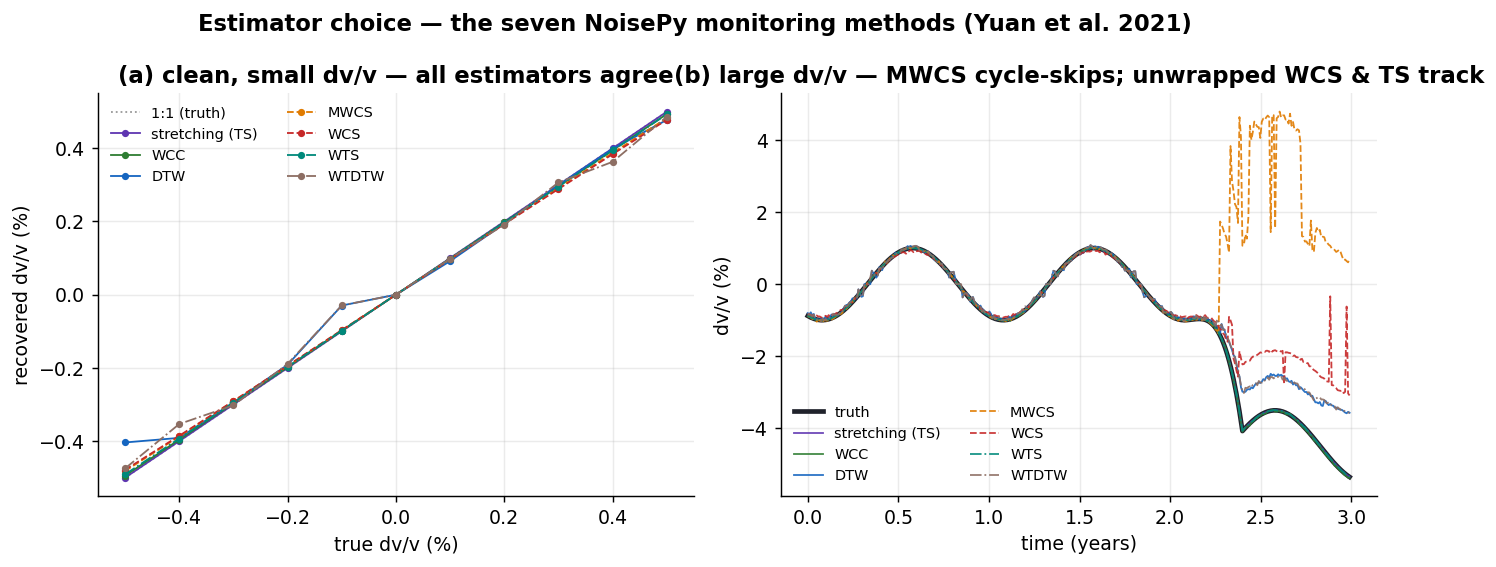
\includegraphics[width=\textwidth]{demo_1_methods.png}
  \caption{Estimator choice across the seven NoisePy methods. (a) Clean,
  small \dvv: all agree. (b) The same clean recovery swept over $\pm 5\,\%$
  true \dvv: MWCS cycle-skips past $\sim\!1.5\,\%$ on either branch; TS and WTS
  track the 1:1 line throughout; WCC tracks just as tightly on the negative
  branch but breaks sharply near the positive edge; DTW and WTDTW break
  asymmetrically, WTDTW near $+1\,\%$ but only near $-3\,\%$ on the other
  branch; WCS degrades smoothly, crossing $1\,\%$ error beyond $\pm 4\,\%$.
  (c) Large, noisy \dvv\ (a pre-failure landslide signal): the stretching
  family and WCC track, the warping methods under-shoot, and both phase
  methods fail (MWCS cycle-skips; WCS loses the phase track in noise despite
  the 2-D unwrapping that carries it through the clean sweep in b). RMS
  errors are given in the text; the plotted arrays are in the figure's
  sidecar (Table~\ref{tab:estimands}).}
  \label{fig:methods}
\end{figure}

On a clean, noiseless sweep of true \dvv~from \(-5\) to \(5\,\%\)
(Fig.~\ref{fig:methods}b), the phase-wrapped MWCS estimator is the first
to break on either branch: its error stays below \(0.1\,\%\) out to
\(\sim\!1.3\,\%\) true \dvv, then exceeds \(1\,\%\) error by
\(\sim\!1.5\,\%\) --- the cycle-skip, essentially symmetric in sign. The
stretching family (TS, WTS) stays below \(0.1\,\%\) error out to the
full \(5\,\%\) tested, on both branches. WCC is just as accurate on the
negative branch (error stays below \(0.1\,\%\) throughout) but breaks
sharply on the positive branch, crossing both \(0.1\,\%\) and \(1\,\%\)
error abruptly at the edge of the tested range (\(\sim\!4.75\,\%\)) ---
a sign asymmetry from the physical convention itself
(Section~\ref{sec:intro}), not a processing artefact. The warping
methods develop large (\(>\!1\,\%\)) errors asymmetrically as the warp
path becomes ill-conditioned: WTDTW crosses \(1\,\%\) error already at
\(\sim\!1\,\%\) true \dvv~on the positive branch but only at
\(\sim\!3\,\%\) on the negative branch, and DTW crosses at
\(\sim\!2.5\,\%\) versus \(\sim\!3\,\%\). WCS degrades smoothly rather
than catastrophically, crossing \(1\,\%\) error beyond \(\pm4\,\%\) true
\dvv~on either branch.

\subsection{Aggregating cross-component results}\label{sec:aggregation}

Each three-component seismic station (e.g., Z, N, E) carries 6
cross-component correlations (ZZ, NN, EE, ZE, ZN, NE), whether they are
calculated at a single station or an inter-station pair. Each carries a
signature of the changes in velocity; components may be dominated by
Love or Rayleigh waves \citep{Lin2008, Stehly2006}, but scattering and
non-straight ray paths induce cross-component leakage between modes
\citep{Hennino2001, Margerin2019}, and thus it is often assumed in
practice that coda waves of cross-components with multi-scattering
characteristics (e.g., no clearly separated phases) are composed of
``surface waves'' with strong S-wave sensitivity. Combining them
together requires parameter choices, such as averaging them directly
\citep{Liu2014}, or weighted (e.g., using coherence-based weighting
\citet{Hobiger2012}, \citet{DePlaen2016}).

Combining is another workflow choice that can change both the value and
the uncertainty (Fig.~\ref{fig:aggregation}). One may peak-pick each
component's correlation-coefficient curve \(\mathrm{CC}(\varepsilon,t)\)
and then average the per-component \dvv~(Approach A) --- unweighted, a
few poor components bias the mean; coherence-weighted, they are
suppressed --- or one may average the \(\mathrm{CC}(\varepsilon,t)\)
\emph{images} across components first and peak-pick once (Approach B).
All three conventions appear in the literature; on the same pair they
give visibly different time series, and they propagate uncertainty along
incompatible pathways (the ensemble spread of the per-component picks
for A, the width of the averaged correlation peak for B). On our
six-component synthetic (three good, three poor SNR), the RMS error
against the known truth is \(\sim\!0.31\,\%\) for unweighted Approach A,
\(\sim\!0.08\,\%\) for coherence-weighted Approach A (the poor
components suppressed, \(\sim\!4\times\) better), and \(\sim\!0.03\,\%\)
for Approach B (averaging the images before peak-picking,
\(\sim\!11\times\) better than the unweighted mean and \(\sim\!3\times\)
better than the weighted one).

\begin{figure}
  \centering
  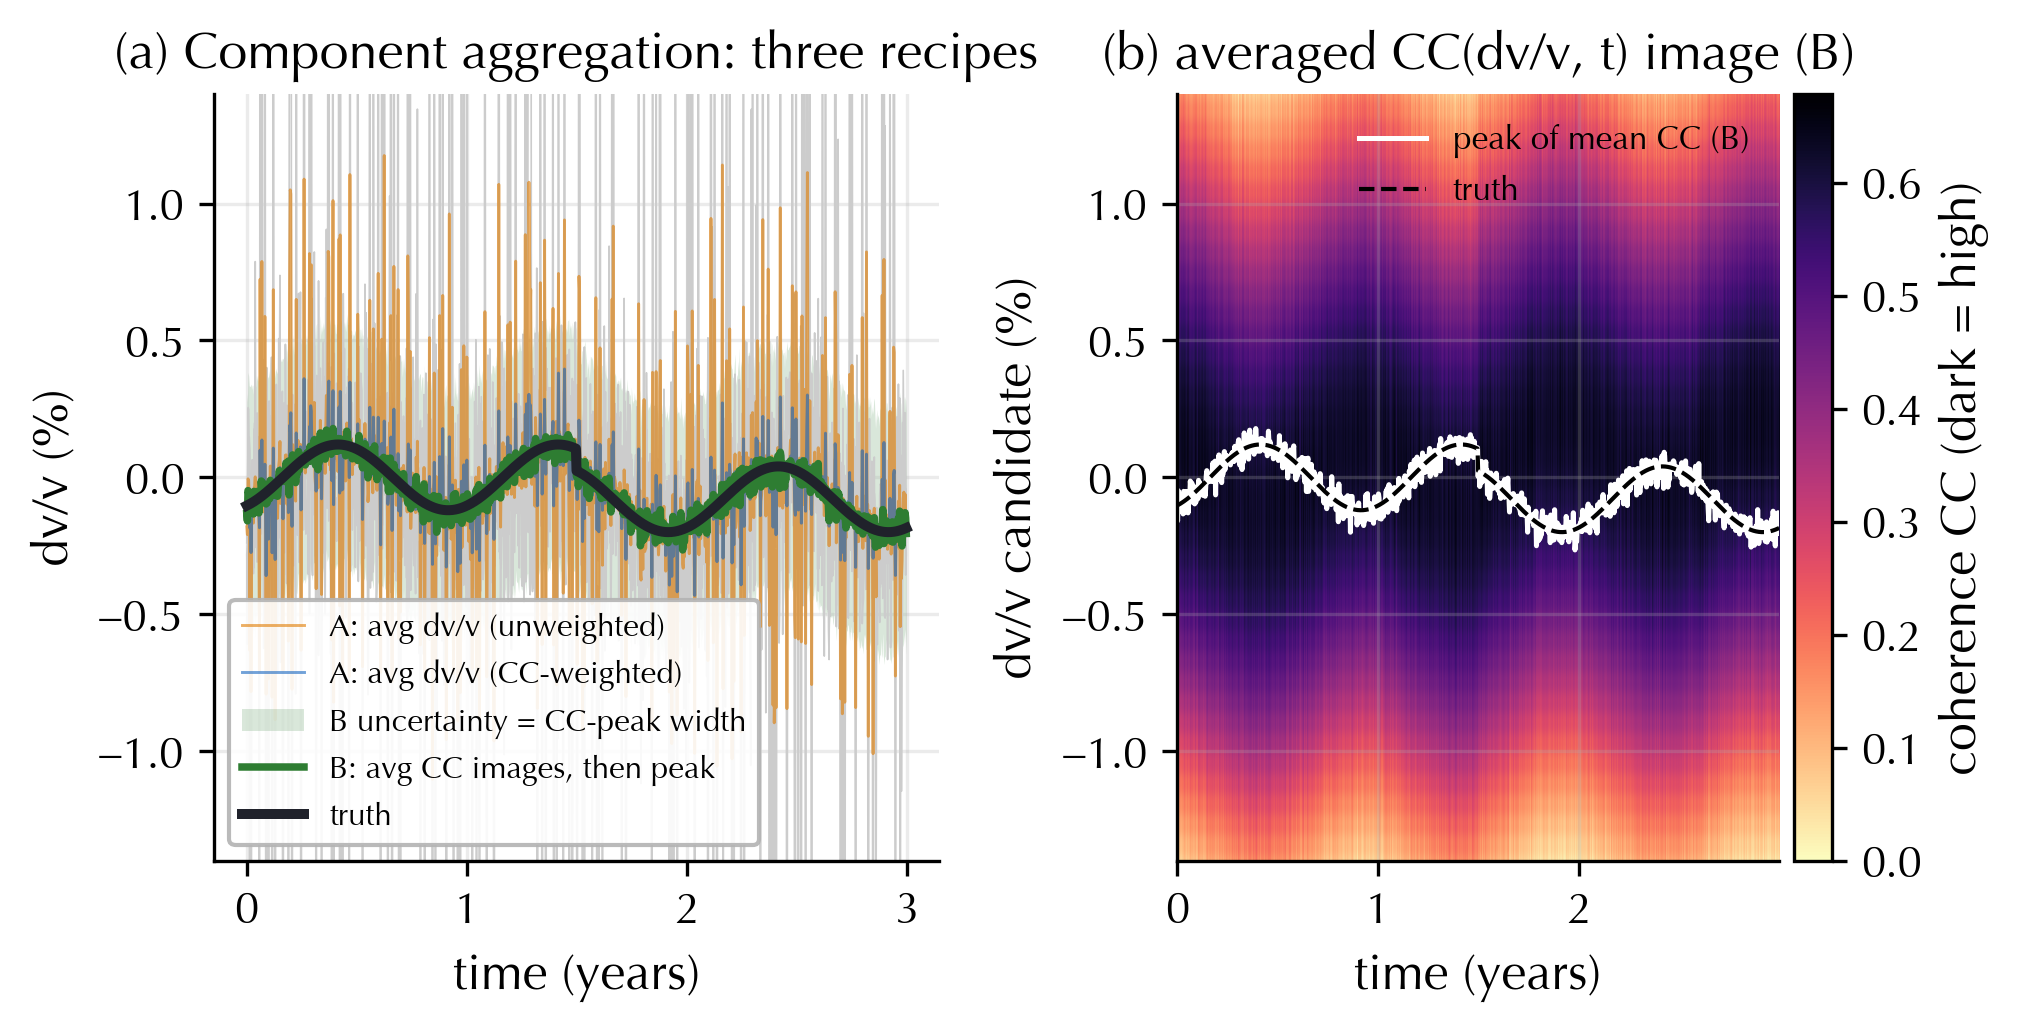
\includegraphics[width=\textwidth]{demo_2_aggregation.png}
  \caption{Cross-component aggregation for one station pair, both panels on the
  same \dvv\ axis. (a) Unweighted \dvv-averaging (Approach A) is biased by the
  poor components (grey), while coherence-weighting and image-averaging
  (Approach B) track the truth; the shaded band is B's local peak-width
  uncertainty. (b) The averaged $\mathrm{CC}(\dvv,t)$ image of Approach B
  (dark = high coherence) with its peak ridge (white) tracking the truth
  (black, dashed).}
  \label{fig:aggregation}
\end{figure}

\subsection{Aggregating across station pairs}\label{sec:uncertainty}

Adding the next layer up --- combining many station pairs into a unified
network series --- exposes the most consequential and least-reported
choice of all: how to summarize the uncertainty. Three conventions are
common: a coherence-weighted standard error (e.g., \citet{Clarke2011}),
an unweighted standard error (\(\sigma=\mathrm{std}/\sqrt{N}\); e.g.,
\citet{Brenguier2008}), and the between-pair standard deviation (e.g.,
\citet{Clements2018}). These are estimates of different quantities
(Table~\ref{tab:estimands}): the standard error is the precision of the
network mean under independent pairs, the standard deviation is the
dispersion of the pairs, which on this synthetic mixes the \(15\,\%\)
pair-to-pair amplitude heterogeneity we impose with the pair noise, and
the two are related by \(\sqrt{N}\) by construction. On the same
synthetic network the recovered means nearly coincide, but the number
reported as \(1\sigma\) spans a factor of \(\sim\!\sqrt{N}\)
(Fig.~\ref{fig:uncertainty}). A velocity change that is three times the
coherence-weighted standard error is about one between-pair standard
deviation, from identical data; neither statement is wrong, but a study
that reports only ``\(1\sigma\)'' leaves the reader unable to tell which
is meant. Error bars on published \dvv~are therefore not comparable
across studies unless the aggregation, the weighting, and the
standard-error-versus-standard-deviation convention are all stated.
Neither convention is the precision of the mean when pairs share
stations or noise; that requires the pair covariance,
\(\mathbf{a}^\top\Sigma\mathbf{a}\) for normalised weights
\(\mathbf{a}\), which the Bayesian ensemble of Section~\ref{sec:bayes}
supplies for the configuration axis and which a network extension would
supply for the pair axis.

\begin{figure}
  \centering
  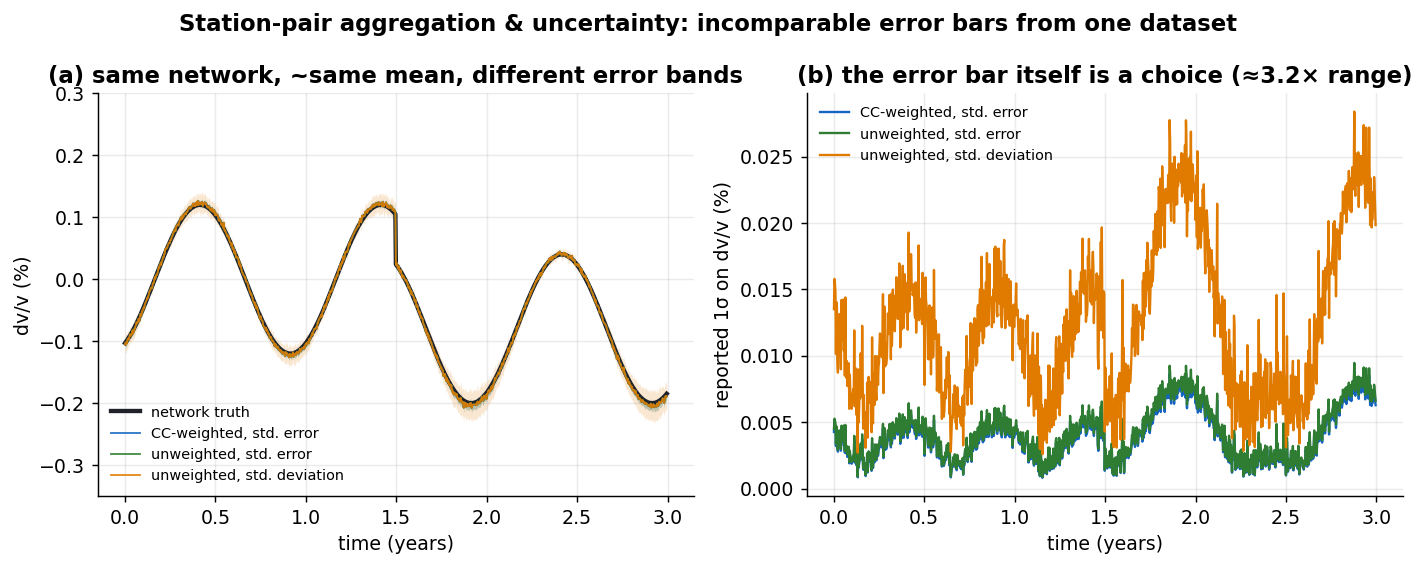
\includegraphics[width=\textwidth]{demo_3_uncertainty.png}
  \caption{Station-pair aggregation and uncertainty for a nine-pair network. (a)
  The recovered \dvv\ agrees across conventions; the shaded $1\sigma$ bands do
  not. (b) The reported $1\sigma$ differs by $\sim\!\sqrt{N}$ purely from the
  weighting and SE-versus-SD choices.}
  \label{fig:uncertainty}
\end{figure}

Figure~\ref{fig:uncertainty} plots only the \emph{network-aggregate}
series, which hides how much the individual pairs actually disagree.
Fig.~\ref{fig:network-pairs} plots the same nine-pair network's
\emph{individual} \dvv(t) curves, styled after a basin-scale, urban
ambient-noise deployment such as the San Gabriel Valley groundwater
network \citep{Clements2018} --- an illustrative geometry rather than a
literal reproduction of that network's exact station spacing. The
individual pairs range in quality from a coherence-weighted SNR of
\(\sim\!2.5\) to \(\sim\!11\), and their spread at any given day (median
range \(\sim\!0.053\,\%\)) is nearly \(10\times\) wider than the
coherence-weighted network standard error (median \(\sim\!0.005\,\%\))
and more than \(3\times\) wider than the more conservative between-pair
standard deviation (median \(\sim\!0.017\,\%\)). A network-level error
bar, however it is computed, describes the precision of the \emph{mean},
not the \emph{dispersion} of what individual pairs actually report ---
the two are routinely conflated when a single station-pair result is
compared against a published network value.

\begin{figure}
  \centering
  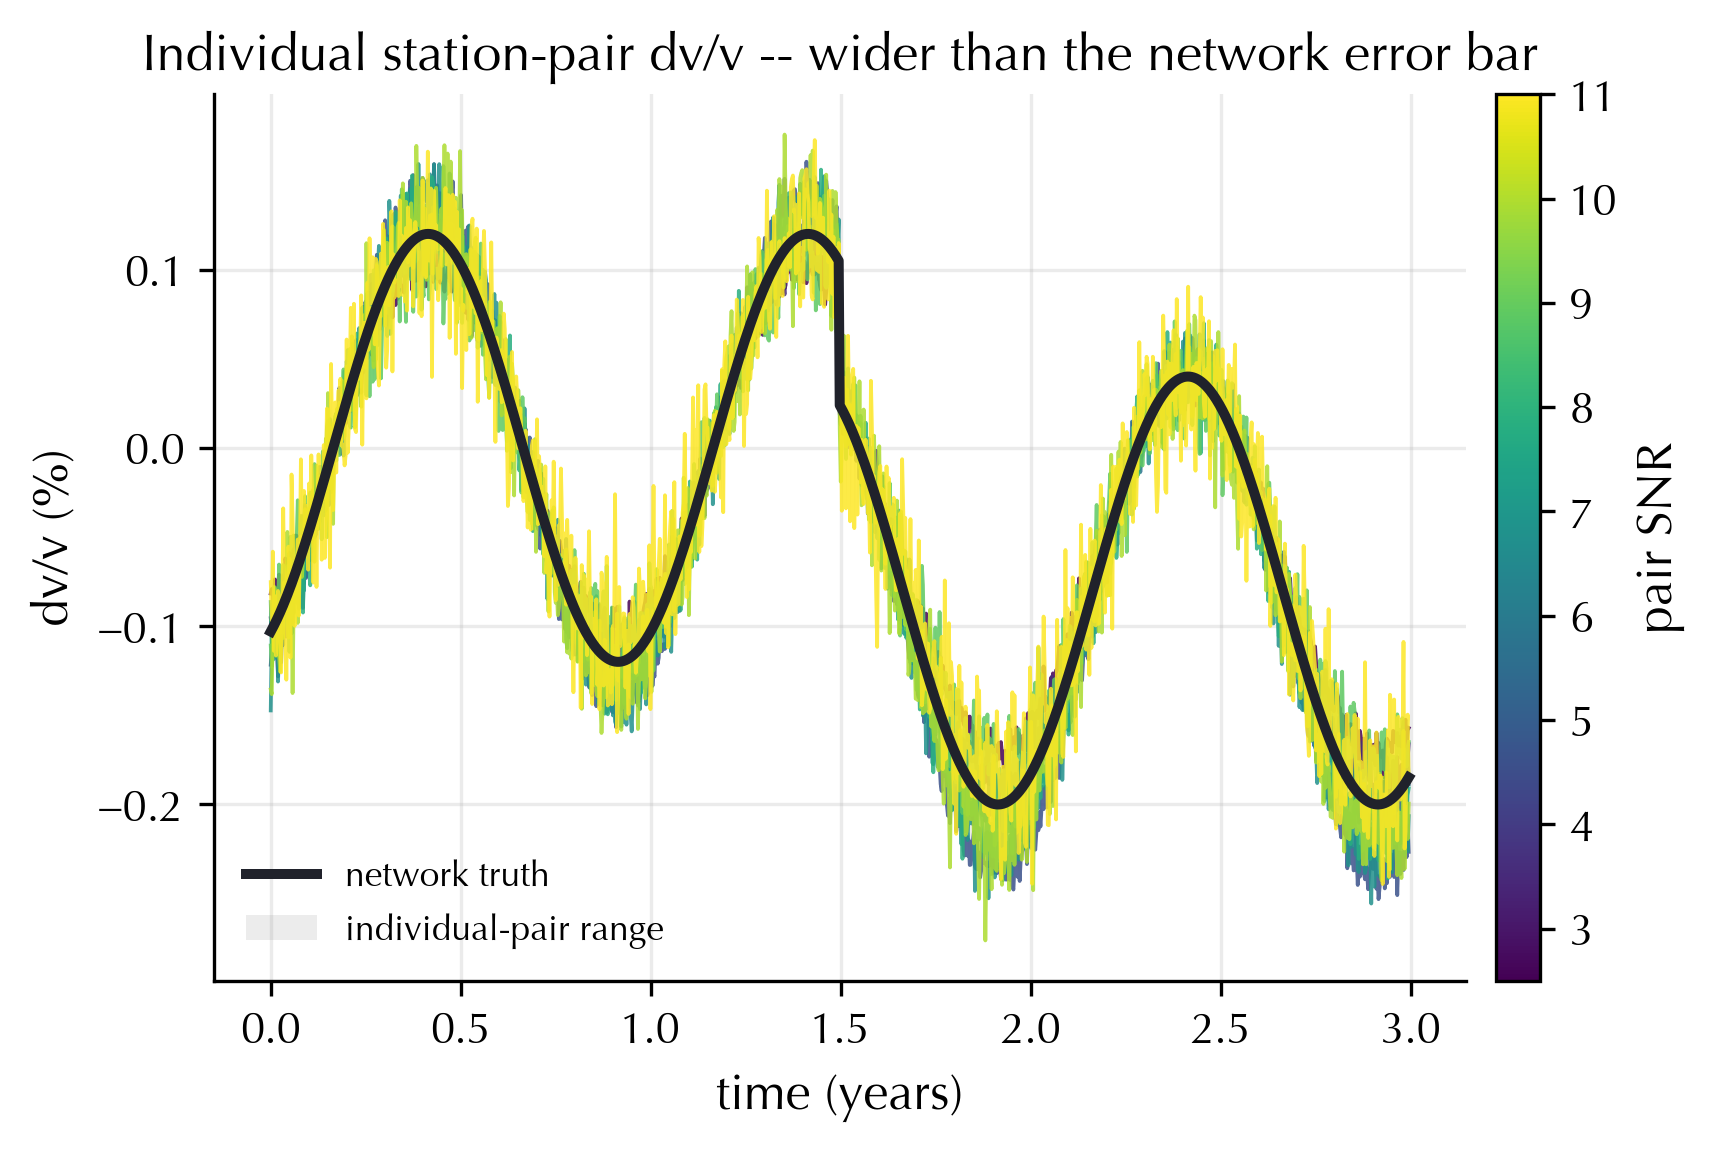
\includegraphics[width=0.75\textwidth]{demo_14_network_pairs.png}
  \caption{Individual station-pair \dvv(t) for the same nine-pair network as
  Fig.~\ref{fig:uncertainty}, coloured by pair SNR. The pair-to-pair spread
  (grey band) is far wider than any of the three network-level $1\sigma$
  conventions in Fig.~\ref{fig:uncertainty}b.}
  \label{fig:network-pairs}
\end{figure}

\subsection{Frequency band}\label{sec:params_freq}

The remaining choices are no less consequential. The \textbf{frequency
band} sets the sampled depth: in a two-layer medium, high frequencies
recover shallow, often seasonal signals and low frequencies recover a
deeper, maybe more tectonic, signal (Fig.~\ref{fig:params}a). In
practice a band often gets reused from a neighboring deployment or an
earlier study at the same site without re-checking that it still matches
the target depth --- exactly the error this section quantifies.

On our synthetic two-layer groundwater scenario, holding the recovery
band's width fixed (0.6\(\,\)Hz) and sweeping its center away from the
deep layer's true 0.2--0.8\(\,\)Hz band shows the cost is not gradual:
RMS error against the known truth stays flat,
\(\sim\!0.028\)--\(0.031\,\%\), for a center offset within
\(\sim\!0.3\,\)Hz of the true center, then rises by a factor of
\(\sim\!3\)--\(4\) once the offset passes \(\sim\!0.5\,\)Hz --- the
point at which the assumed band starts sampling the shallow layer's
signal instead of the deep one --- and plateaus near \(\sim\!0.10\,\%\)
beyond that (Fig.~\ref{fig:band-sensitivity}). The band choice is
forgiving up to the edge of the layer it targets, and expensive
immediately past it, not gradually worse the further off it drifts.

\begin{figure}
  \centering
  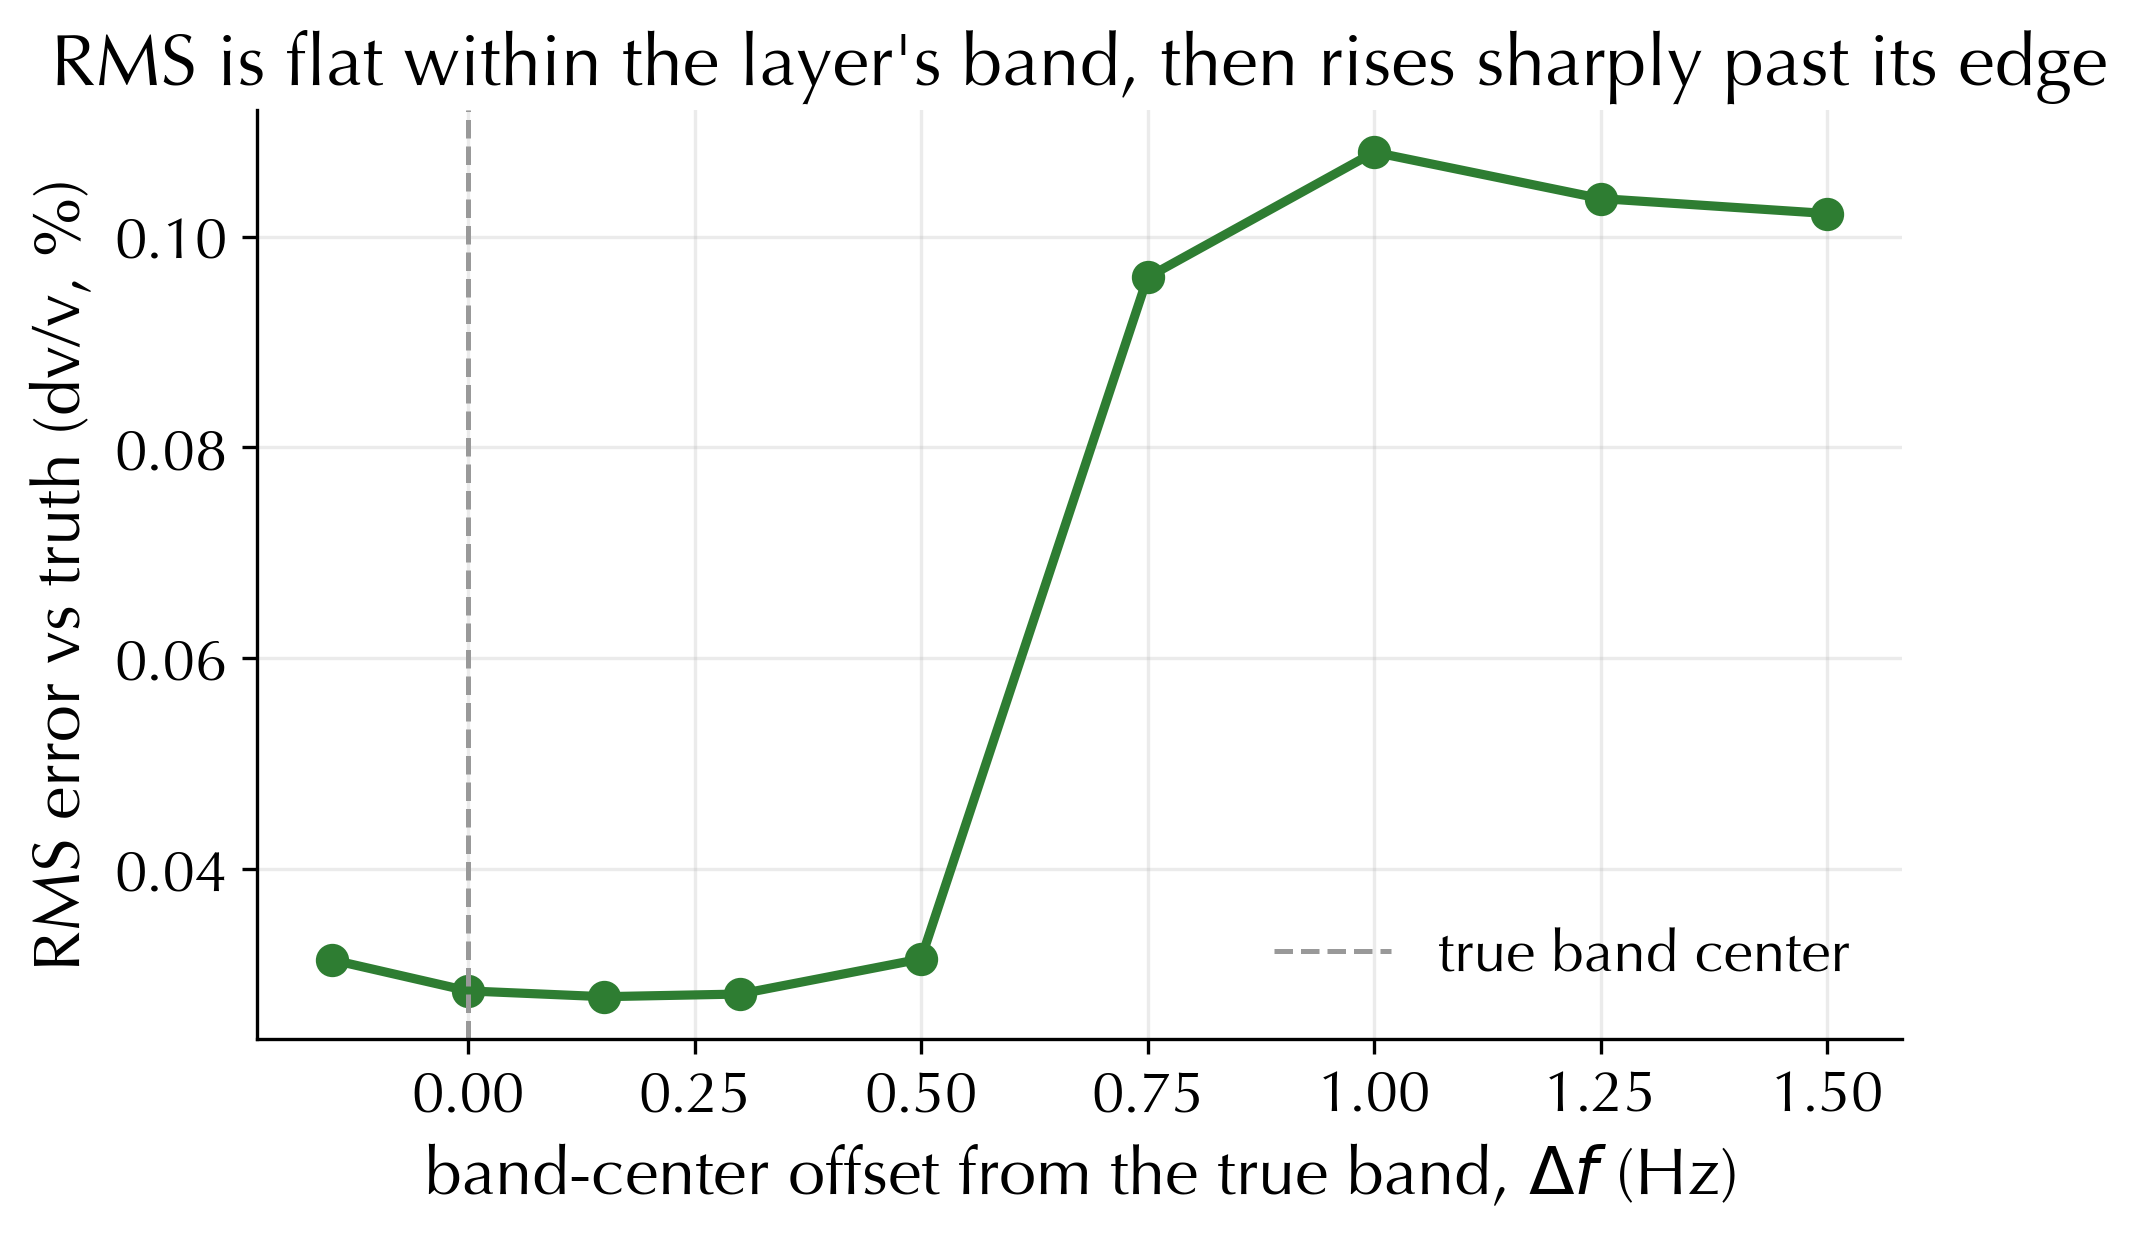
\includegraphics[width=0.7\textwidth]{demo_16_band_sensitivity.png}
  \caption{Frequency-band sensitivity: RMS error against the known
  groundwater deep-layer truth as the recovery band's center is swept away
  from the true 0.2--0.8$\,$Hz band, holding its 0.6$\,$Hz width fixed. Error
  is flat within $\sim\!\pm0.3\,$Hz of the true center, then rises sharply
  once the assumed band drifts into the shallow layer's territory.}
  \label{fig:band-sensitivity}
\end{figure}

\textbf{Scale of effect:} a band-center error under \(\sim\!0.3\,\)Hz
costs essentially nothing here; past \(\sim\!0.5\,\)Hz it costs a factor
of \(\sim\!3\)--\(4\) in RMS, from \(\sim\!0.03\,\%\) to
\(\sim\!0.10\,\%\).

\subsection{Reference}\label{sec:param_ref}

The \textbf{reference} defines what survives: a moving reference
re-baselines continuously and erases slow trends that a fixed reference
or a joint inversion \citep{Brenguier2014} preserve
(Fig.~\ref{fig:params}c). In practice the choice is rarely just
fixed-versus-moving: an analyst also decides \emph{which} period of the
record a fixed reference is built from, and that choice alone can
dominate the error --- for instance when a deployment barely predates
the process of interest, or when the only quiet-looking period available
sits close in time to the process itself.

We compare five named schemes on the volcano synthetic: a reference
built from the \textbf{beginning} of the pre-eruptive record (its
earliest 15\%), from the \textbf{end} of that record (its latest 15\%,
immediately before the eruption), from the \textbf{whole} pre-eruptive
record, a 60-day \textbf{moving} (trailing) reference, and \textbf{no
single reference at all} --- the Brenguier et al. (2014)-style joint
inversion, which measures relative dv/v between many short stacks
instead of referencing every day to one
(Fig.~\ref{fig:reference-schemes}a). The whole-record, beginning, and
inversion schemes all recover the truth to RMS \(\sim\!0.03\,\%\). The
end-of-record reference does far worse, RMS \(\sim\!0.15\,\%\) --- not
because it tracks the dynamics any less faithfully (its residual scatter
around the truth, \(\sim\!0.029\,\%\), matches every other fixed scheme)
but because the reference epoch itself already sits \(\sim\!0.15\,\%\)
into the developing pre-eruptive ramp, and every dv/v value is reported
\emph{relative to whatever the reference was doing}. Reference choice
sets the zero point, not just the noise floor: comparing dv/v across
studies, or across deployments that started at different times, requires
knowing what the reference period itself was doing, not just how well
each pipeline scores against a single truth.

The 60-day moving reference gives RMS \(\sim\!0.16\,\%\) --- comparable
to the worst fixed case, but for the opposite reason: it re-baselines
away the trend continuously rather than sitting at one biased epoch.
Lengthening the trailing window helps only slowly and never converges to
the fixed-reference baseline: RMS falls from \(\sim\!0.168\,\%\) at a
10-day trailing window to \(\sim\!0.151\,\%\) at 240 days, still
\(\sim\!4\)--\(5\times\) the whole-record RMS
(Fig.~\ref{fig:reference-schemes}b) --- the erasure is structural, not a
noise effect that more averaging fixes.

Read carefully, though, that erasure is a property of the
\emph{uncumulated
increment}, not of a non-fixed reference as such --- and the published
alternatives to a fixed reference do not take the form the sweep
assumes. They fall into two families, neither of which re-baselines
every epoch and reports the raw increment.

The first cumulates. \citet{James2017} re-baseline each day against the
immediately preceding day-stack and sum the daily \(\delta t/t\) from a
fixed start date, recovering a seasonal freeze--thaw trend in Alaskan
permafrost that a stationary reference could not detect at all: the
frozen-to-thawed velocity contrast made the stationary comparison
cycle-skip, while adjacent days stayed coherent. \citet{Rivet2011}
likewise reference each epoch to the previous one. The cost is that
summation integrates the measurement error --- \citet{James2017} report
a positive drift in the cumulated series that their quadrature error
budget could not account for, and correct it linearly against a
stationary-reference anchor. The same rolling construction appears in
laboratory coda monitoring of rock deforming to failure, where the
scattering properties change too much for a fixed reference to stay
valid \citep{ZotzWilson2019}.

The second holds the reference fixed within a segment and stitches the
segments together. \citet{Rivet2014} define a separate reference stack
for each of three multi-year periods at Piton de la Fournaise, then
merge the three series by measuring the relative velocity change
\emph{between} the adjacent segment references, using station pairs that
occupied the same sites across the network change.
\citet{SensSchonfelder2014} develop the multiple-reference form of the
same idea at the same volcano, and \citet{Ermert2023} adopt a
multiple-reference approach for urban single-station autocorrelations in
Mexico City, where long-term waveform coherence is simply unavailable,
stabilising the stacks by clustering correlation windows with a Gaussian
mixture model so that day-time and night-time noise regimes stack
separately.

That second family is worth naming precisely, because it is not a
separate method from the joint inversion --- it is a restriction of it.
Stitching two segments by measuring the relative dv/v between their
references is exactly the adjacent-pair case of the over-determined
system the inversion solves over all pairs of block stacks. The
reference axis is therefore better read as a single continuum, from one
global reference, through segment references joined pairwise, to the
fully coupled inversion, than as a menu of unrelated choices.

Against that, the uncumulated day-by-day trailing reference swept above
is a limit case rather than a practice: we found no surveyed study that
re-baselines continuously and reports the increments without summing
them. It is retained here because it isolates what re-baselining costs
when the trend is not reconstructed, which is the failure mode the two
families above exist to avoid. codameter implements the joint inversion
but neither the cumulated trailing reference nor cluster-based reference
selection.

\begin{figure}
  \centering
  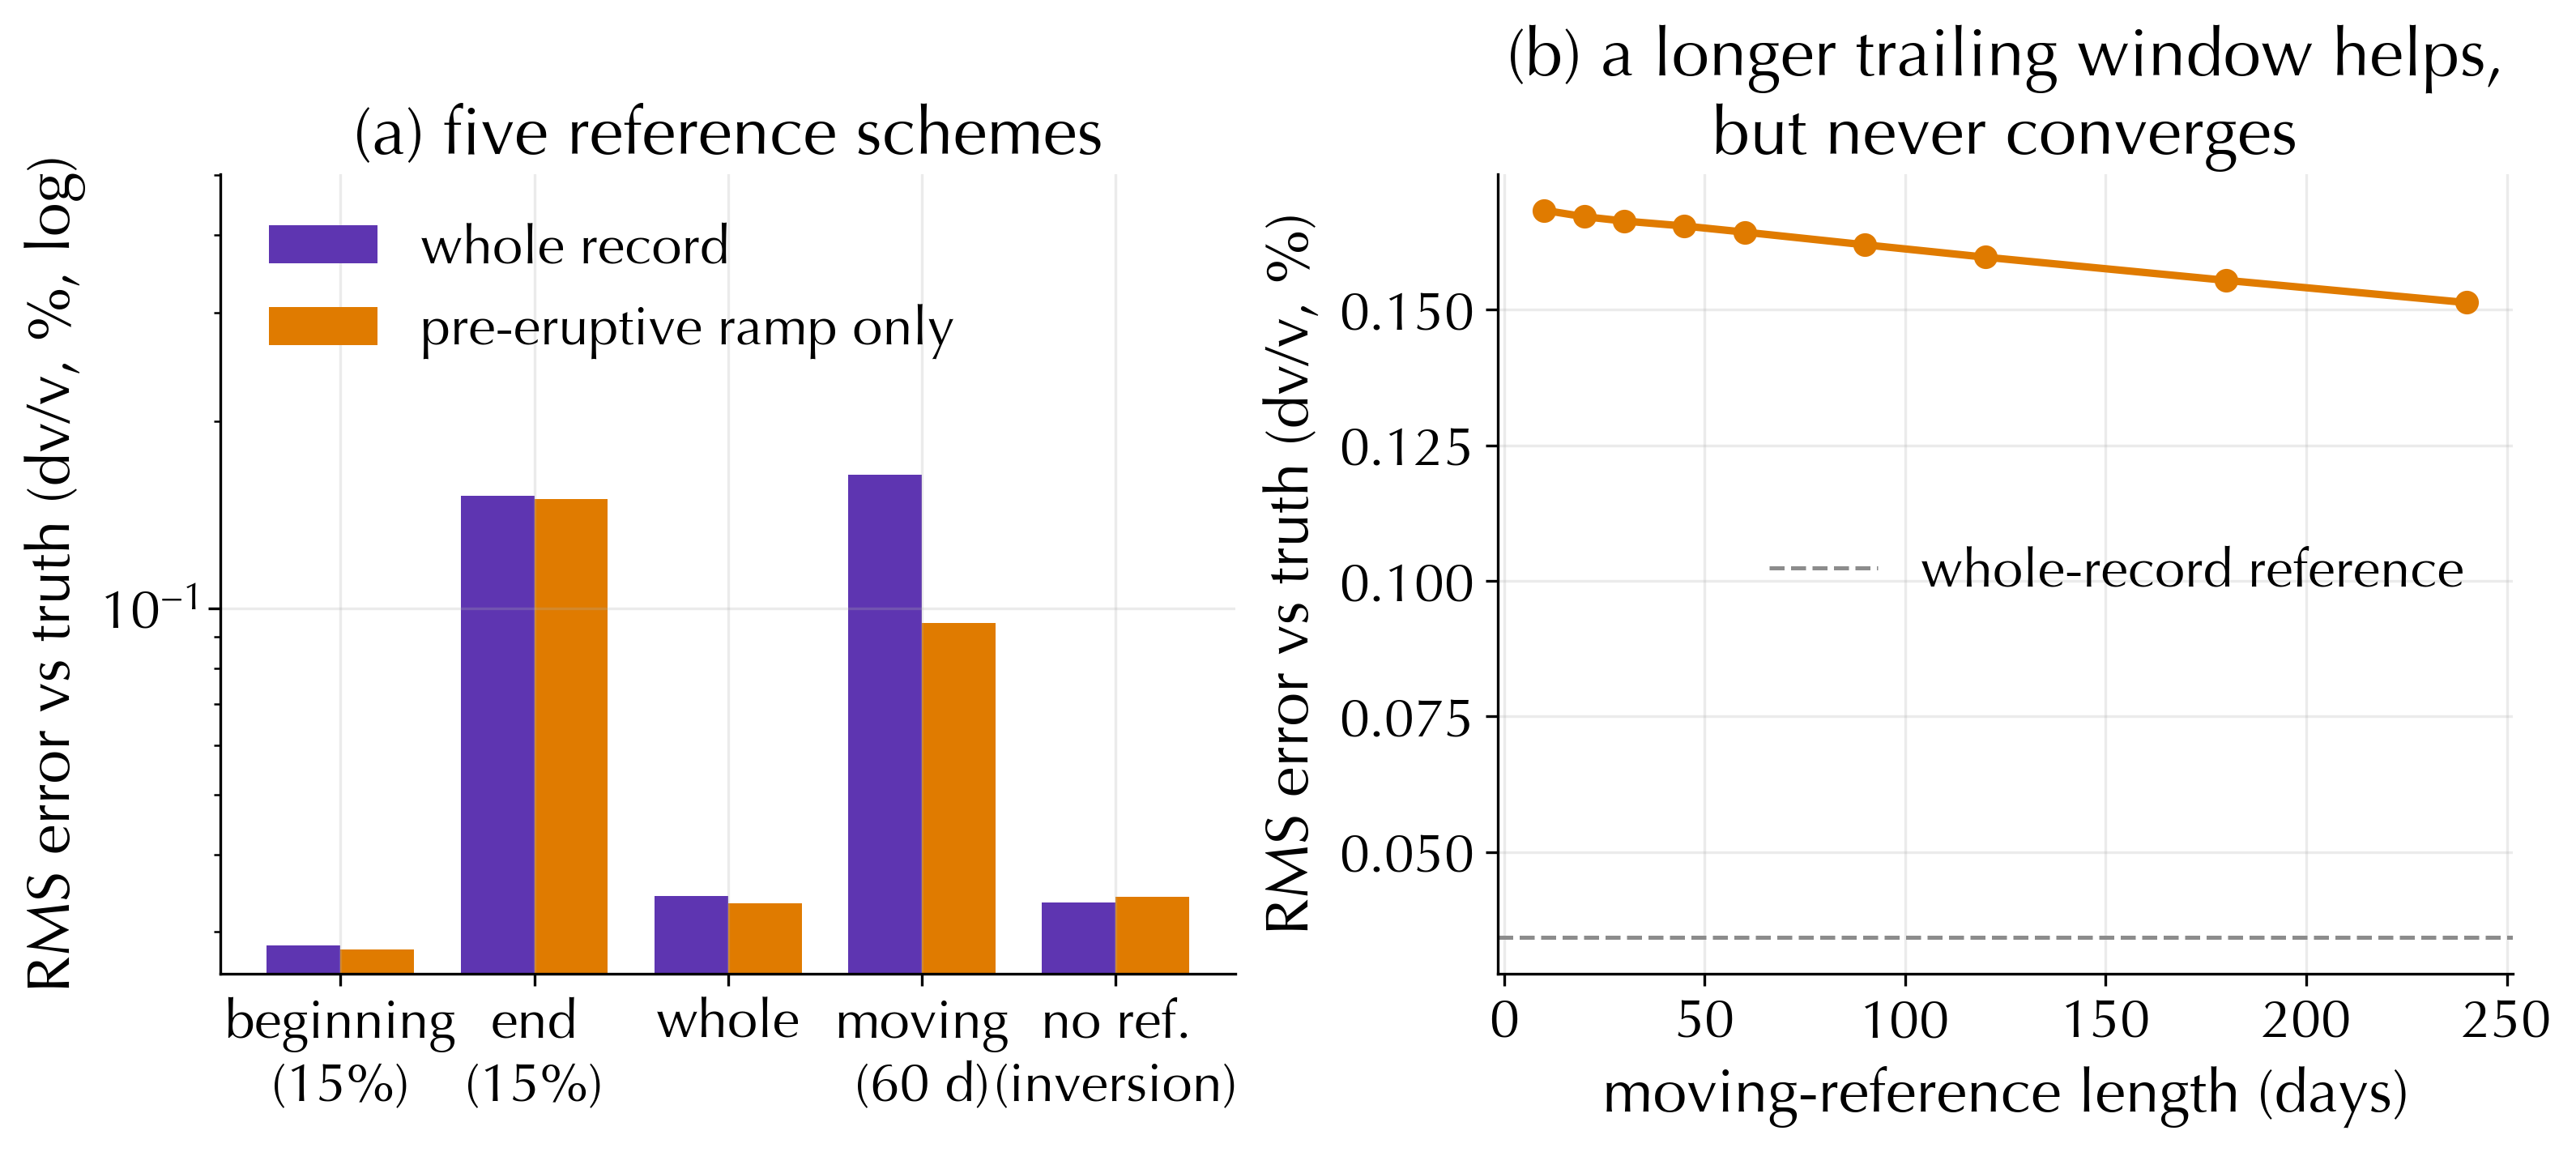
\includegraphics[width=\textwidth]{demo_17_reference_schemes.png}
  \caption{Reference construction on the volcano synthetic. (a) Five named
  schemes, each scored by RMS against the known truth over the whole record
  and over the pre-eruptive ramp alone. (b) RMS for the moving reference as a
  function of its trailing length; the dashed line is the whole-record fixed
  reference's RMS, which the moving reference never reaches.}
  \label{fig:reference-schemes}
\end{figure}

\textbf{Scale of effect:} which \emph{period} a fixed reference is drawn
from can cost as much as switching to a moving reference altogether
(\(\sim\!0.15\)--\(0.16\,\%\) RMS either way); a reference from the
quietest available period, of any length, recovers the trend to
\(\sim\!0.03\,\%\).

\subsection{Substacking}\label{sec:param_substack}

The \textbf{stacking length} trades noise against temporal resolution,
rounding off and delaying a coseismic step (Fig.~\ref{fig:params}d). In
practice the decision is rarely ``how many days'' in the abstract; it is
``how long until the coda is coherent enough to trust'' --- stacking
only as long as needed to clear a working correlation-coefficient (CC)
threshold, then stopping. codameter's own quality-control gate uses
CC\textasciitilde{}\(>0.6\) (Section~\ref{sec:results}), and how quickly
a station clears that bar depends entirely on its data quality.

Substack duration therefore defines a fundamental
precision--temporal-resolution tradeoff. Longer stacks suppress
incoherent noise fluctuations and accelerate the convergence of noise
correlation functions, whereas shorter substacks preserve transient
changes that would otherwise be averaged within the stacking window. The
reduced signal-to-noise ratio of shorter correlations can be partially
compensated through adaptive filtering, SVD-based or learned denoising,
or through redundancy across dense seismic arrays, enabling
\dvv~measurements at daily, hourly, and even sub-hourly resolution
\citep[\citet{Moreau2017},\citet{Mao2019},\citet{Viens2020}]{Hadziioannou2011}.

In this paper, the choice of substack length is guided by data-dependent
quality gates (the CC threshold above) rather than a fixed duration,
which allows stations with high coherence to preserve shorter temporal
windows and thereby track rapid changes, while stations with lower SNR
substack as needed to achieve stable estimates.

On the earthquake synthetic, a workable deployment (SNR 4, the same
setting used throughout this section) clears CC\textasciitilde{}\(>0.6\)
already at a 1-day stack (median CC 0.86); a poor, coherence-limited
deployment (SNR 0.5) needs 14 days of substacking to clear the same bar
(Fig.~\ref{fig:stack-coherence}a). The two regimes behave differently
past that point, too. For the workable deployment, RMS is U-shaped: it
falls from \(\sim\!0.044\,\%\) at 1 day to a minimum \(\sim\!0.020\,\%\)
around 7--10 days, then rises again to \(\sim\!0.038\,\%\) by 60 days as
the stack smears the step (Fig.~\ref{fig:stack-coherence}b) --- the
classic noise-versus-smearing tradeoff, and the reason ``longer is
always better'' is wrong even once the coherence gate is satisfied. For
the poor deployment, RMS is still falling at 60 days
(\(\sim\!0.067\,\%\), down from \(\sim\!0.74\,\%\) at 1 day): the noise
floor dominates over the whole tested range, and the smearing penalty
never gets the chance to show up. The signed error in the recovered step
amplitude is negative (an under-estimate) at every stack length for the
poor deployment, and for the workable deployment up to about 45 days,
past which it crosses zero and the step is over-estimated. A recovered
step is therefore a lower bound on the true drop only in the
noise-limited regime; the sign of the error depends on the deployment
and the stack length, and both should be reported.

\begin{figure}
  \centering
  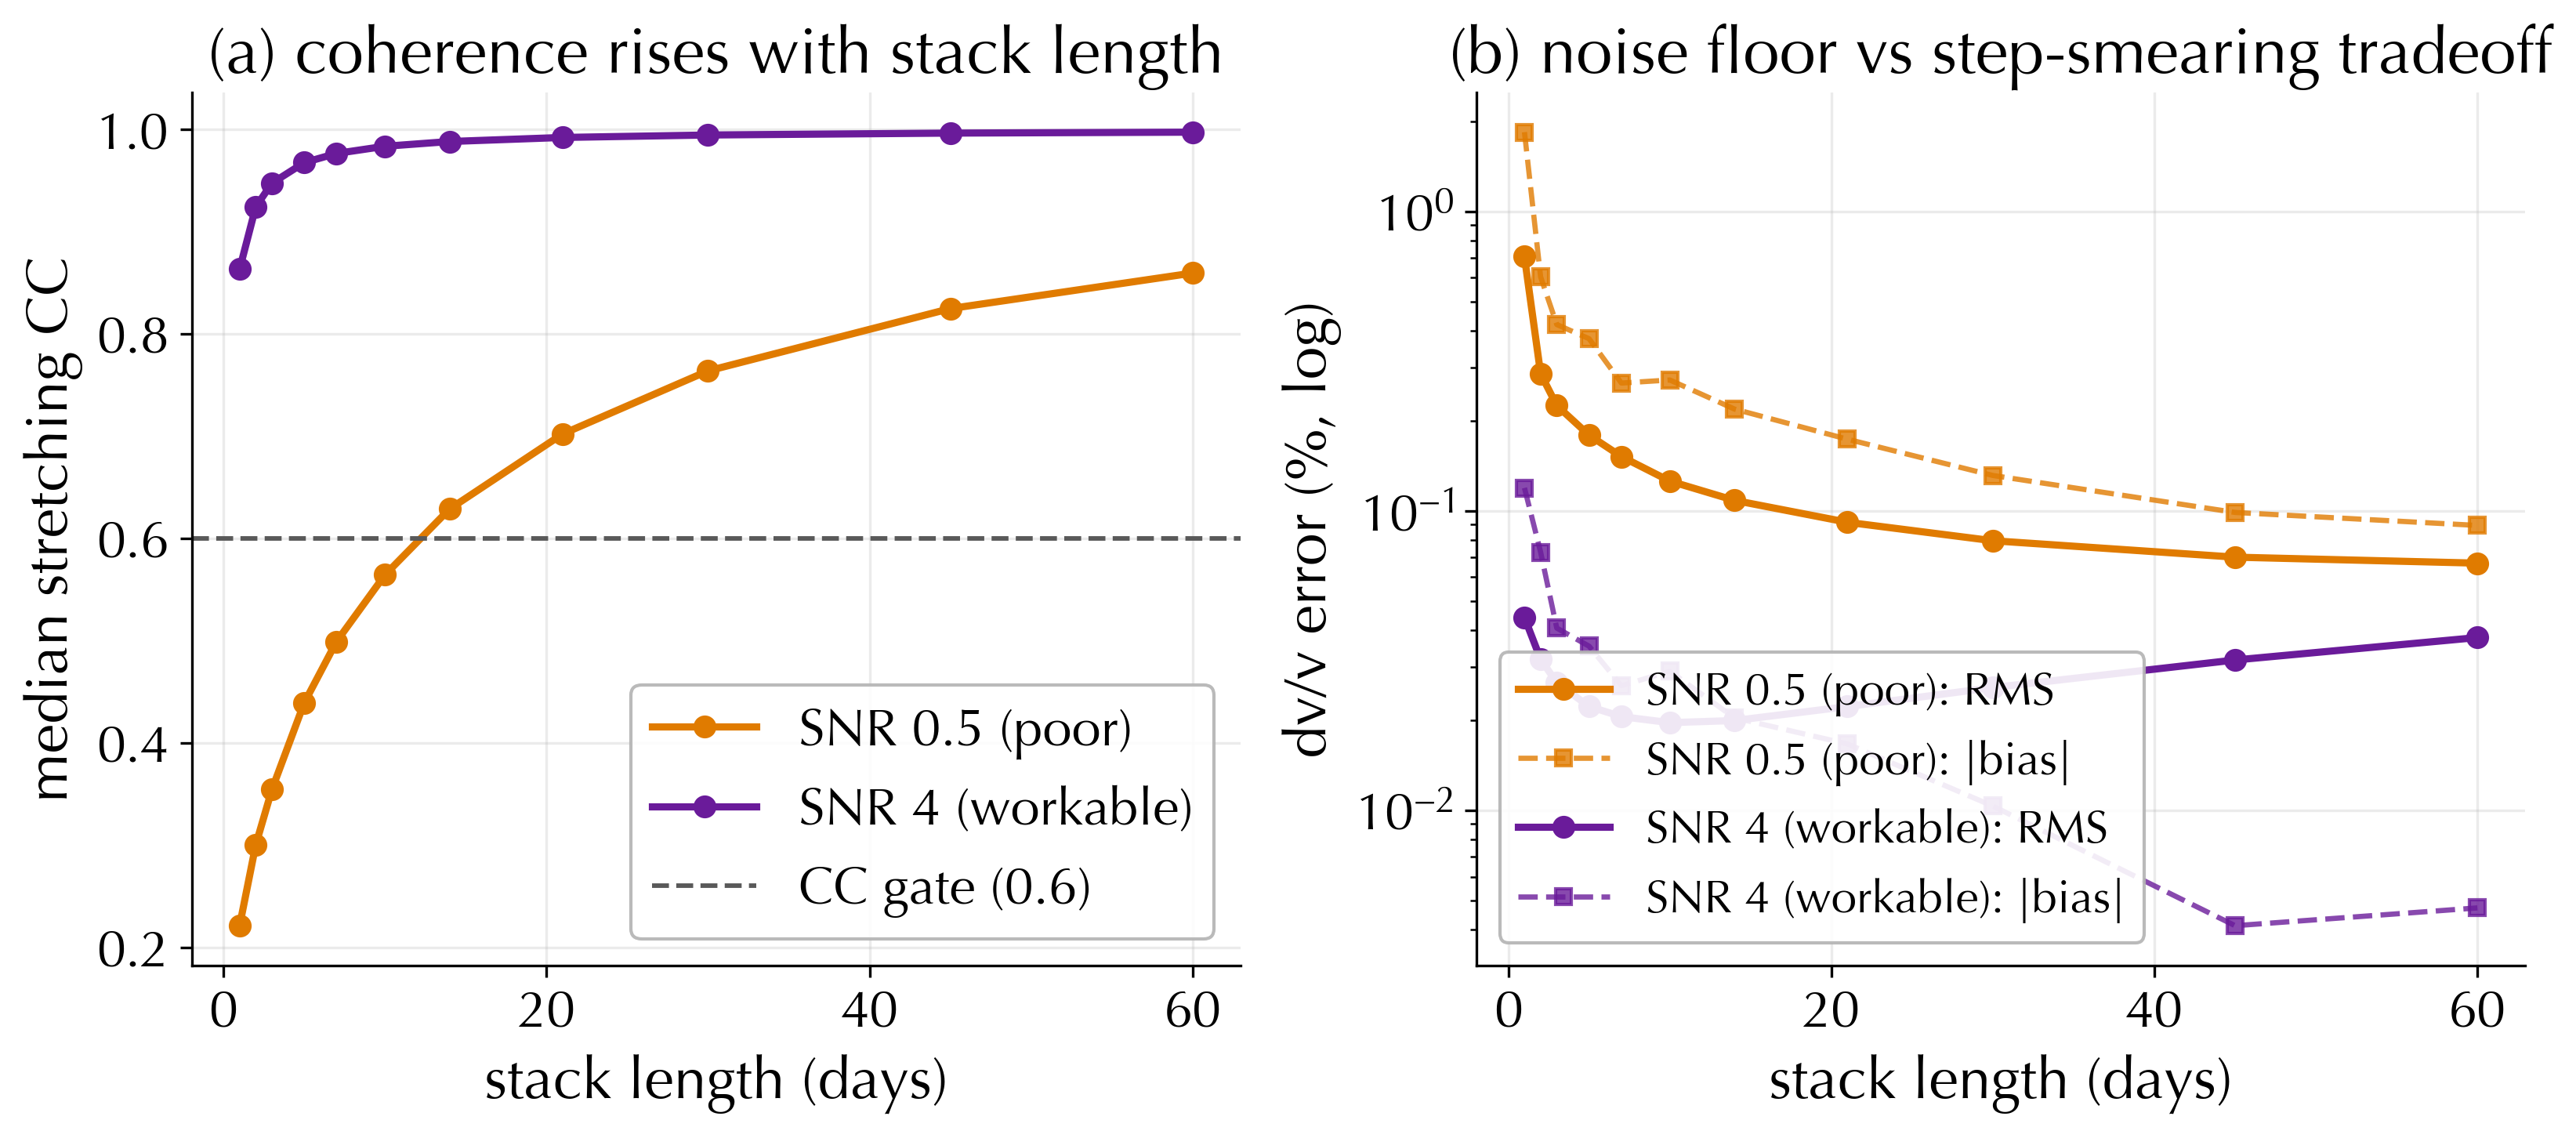
\includegraphics[width=\textwidth]{demo_18_stack_coherence.png}
  \caption{Substacking on the earthquake synthetic, at two deployment
  qualities. (a) Median stretching correlation coefficient versus stack
  length; the dashed line is codameter's own CC-gate threshold
  (Section~\ref{sec:results}). (b) RMS error and the absolute bias in the
  recovered coseismic-step amplitude, both against the known truth, log
  scale.}
  \label{fig:stack-coherence}
\end{figure}

\textbf{Scale of effect:} for a workable deployment, the noise/smearing
tradeoff bottoms out around 7--10 days at RMS \(\sim\!0.02\,\%\); for a
poor deployment, substack at least \(\sim\!2\) weeks just to clear the
coherence gate, and expect RMS an order of magnitude worse even after
clearing it.

\begin{figure}
  \centering
  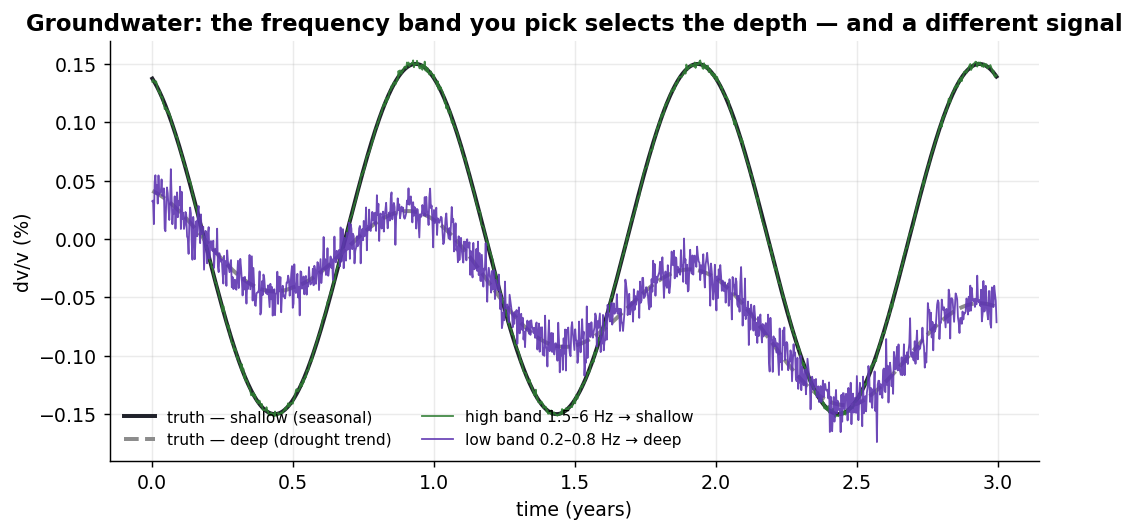
\includegraphics[width=0.49\textwidth]{demo_4_frequency_depth.png}\hfill
  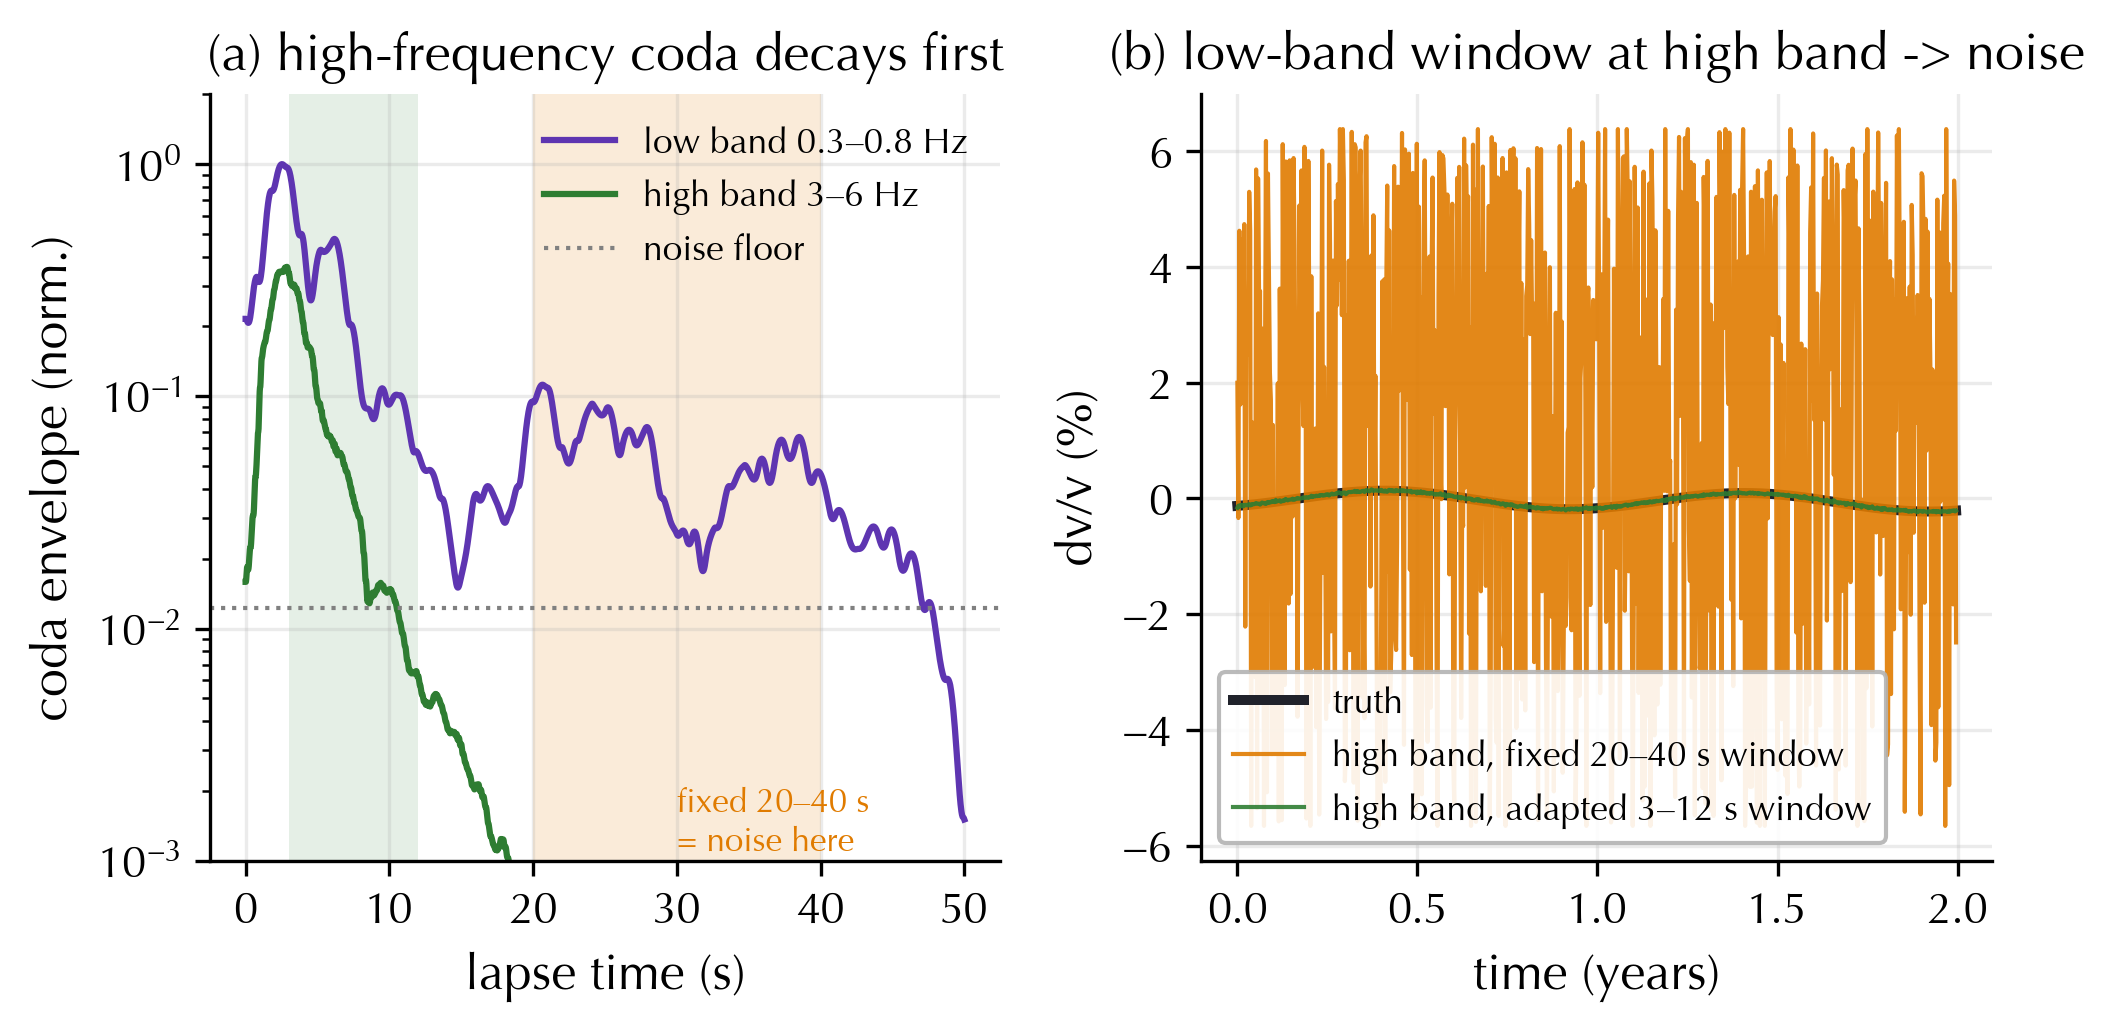
\includegraphics[width=0.49\textwidth]{demo_5_window_band.png}\\[2pt]
  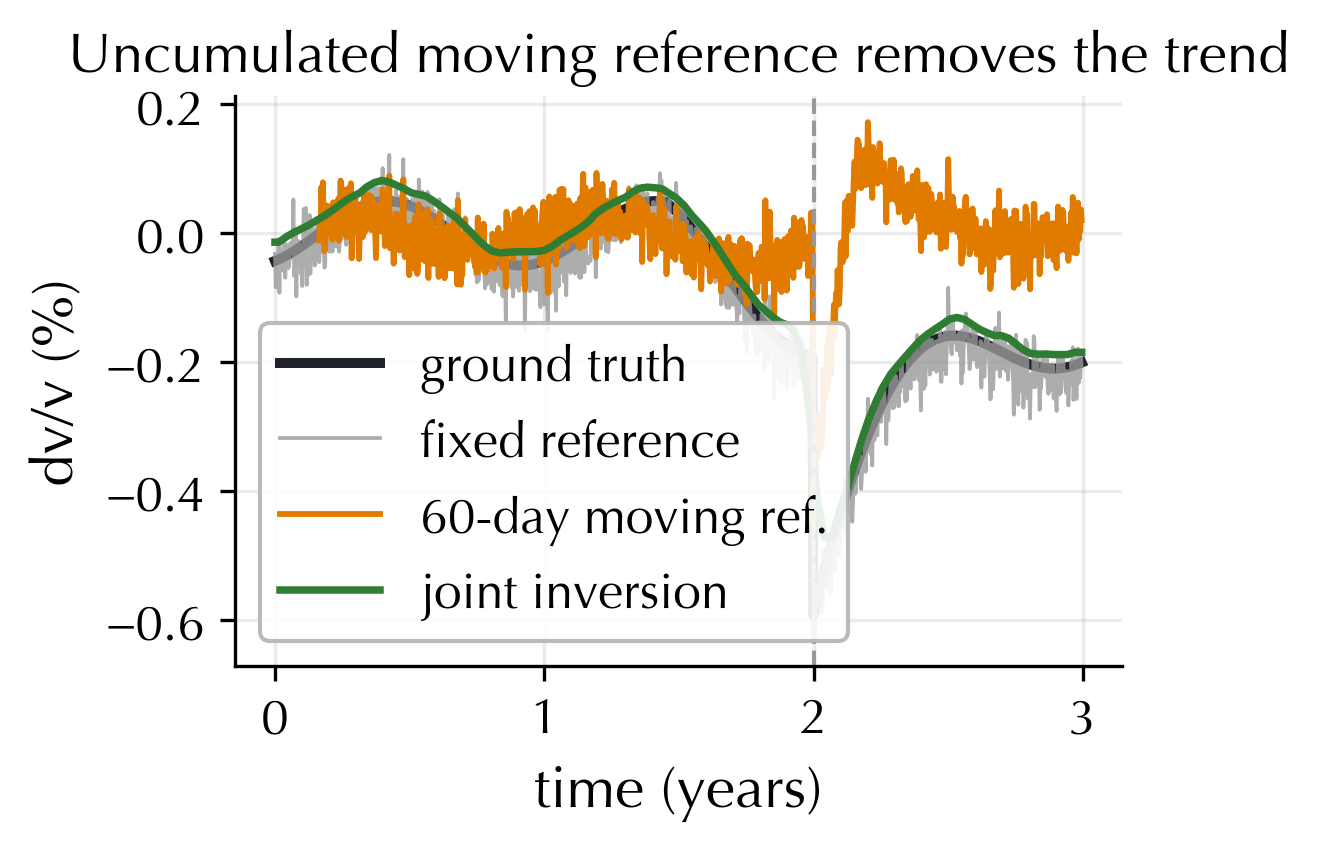
\includegraphics[width=0.49\textwidth]{demo_7_reference.png}\hfill
  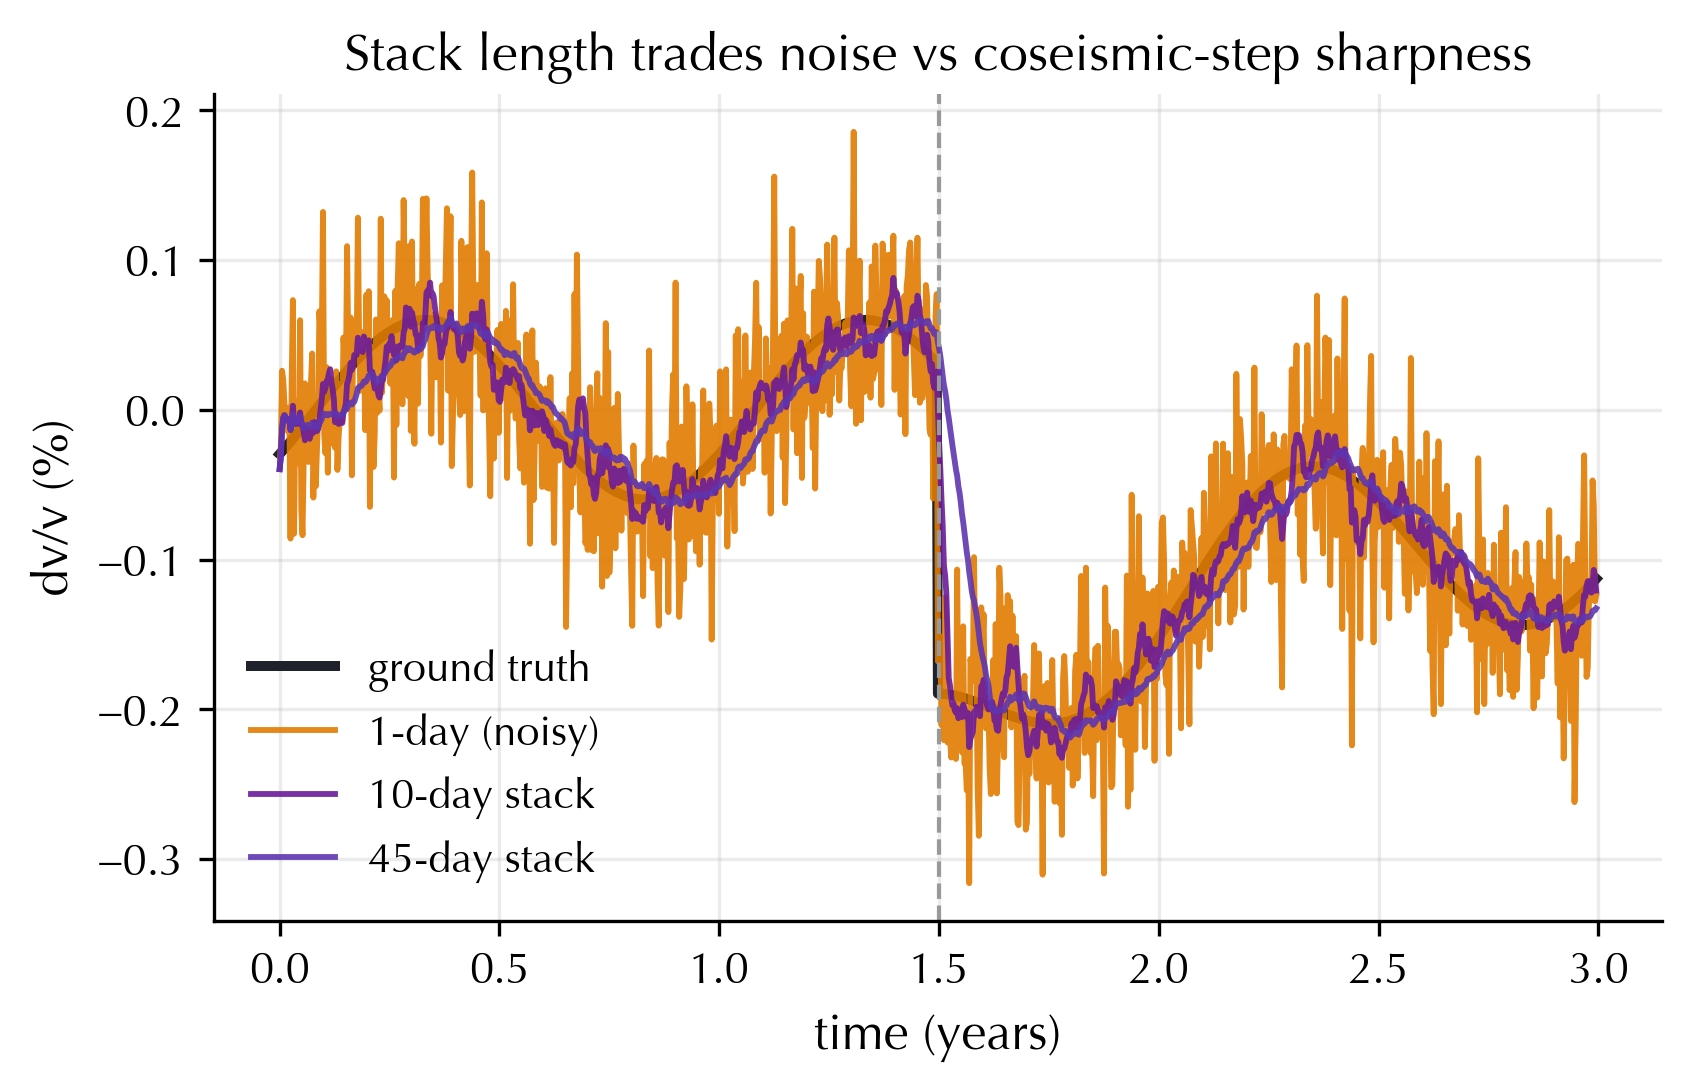
\includegraphics[width=0.49\textwidth]{demo_6_stacking.png}
  \caption{Parameter choices. (a) Frequency band selects depth and signal. (b)
  A coda window does not transfer across bands. (c) Reference strategy: a moving
  reference differences the trend away unless its increments are cumulated;
  a fixed reference and the joint inversion retain it. (d)
  Stacking length smears the coseismic step.}
  \label{fig:params}
\end{figure}

The accepted range for each of these parameters across the published
literature is catalogued directly, study by study, in the survey of
Appendix~\ref{app:survey} (Table~\ref{tab:survey}): the frequency band,
coda window, estimator, and uncertainty treatment actually reported by
103 ambient-noise \dvv~studies.

\subsection{Coda window}\label{sec:param_window}

The coda window is not independent of the frequency band --- it deserves
its own treatment because the two covary strongly, and getting this
wrong is one of the larger, more avoidable sources of error in
\S\ref{sec:results}. Because intrinsic and scattering attenuation both
grow with frequency, high-frequency coda energy falls into the noise
floor much sooner than low-frequency coda: a coda window that is well
past the direct arrival for a \(\sim\!0.3\)--\(0.8\,\)Hz band is, at
\(\sim\!3\)--\(6\,\)Hz, sampling almost pure noise
(Fig.~\ref{fig:params}b). On our synthetic, a fixed 20--40\(\,\)s window
at the high band gives RMS error \(\sim\!3.9\,\%\) (the noise floor, not
the signal), while a window hand-adapted to the band (3--12\(\,\)s)
recovers the truth at \(\sim\!0.01\,\%\) --- nearly a 400\(\times\)
difference from this one choice alone. This is itself an instance of a
literature-documented tension: band-matched windowing is recommended,
but Table~\ref{tab:survey} shows many surveyed studies instead reuse one
fixed window across bands.

Hand-adapting the window per band, as above, requires knowing the band
in advance and re-tuning per deployment. A more principled alternative
--- used in our group --- is to track the coda envelope directly and
stop the window where it \emph{flattens} onto the noise floor, rather
than pre-specifying a window from a rule of thumb. We implement this by
band-passing a long-term reference stack, smoothing its envelope,
estimating the noise floor from a common late-lapse window, and taking
the window end as the first lapse time past a short onset where the
envelope stays within a factor of that floor for a sustained interval
(not a single noisy dip). Applied blind (without being told which band
it is) to three bands spanning low, mid, and high frequency
(Fig.~\ref{fig:window-envelope}a), the detector recovers windows of
\(\sim\!(3,29)\,\)s, \(\sim\!(3,37)\,\)s, and \(\sim\!(3,14)\,\)s
respectively --- correctly shrinking at the high band, though the
low-versus-mid ordering is not perfectly monotonic on this synthetic (an
artifact of how the fixed additive noise floor interacts with each
band's filter, not a claim that the detector is exact). Recovering
\dvv~with each band's own detected window instead of one universal fixed
(10--30\(\,\)s) window (Fig.~\ref{fig:window-envelope}b) gives RMS
\(\sim\!0.030\,\%\) vs.~\(\sim\!0.036\,\%\) at the low band (a modest,
\(\sim\!1.2\times\) gain), \(\sim\!0.017\,\%\) vs.~\(\sim\!0.035\,\%\)
at the mid band (\(\sim\!2\times\)), and \(\sim\!0.020\,\%\)
vs.~\(\sim\!2.0\,\%\) at the high band (\(\sim\!100\times\)) --- the
fixed window is adequate at low frequency and catastrophic at high
frequency, while the envelope-derived window is close to the best
achievable at every band without ever being told what band it is
measuring.

\begin{figure}
  \centering
  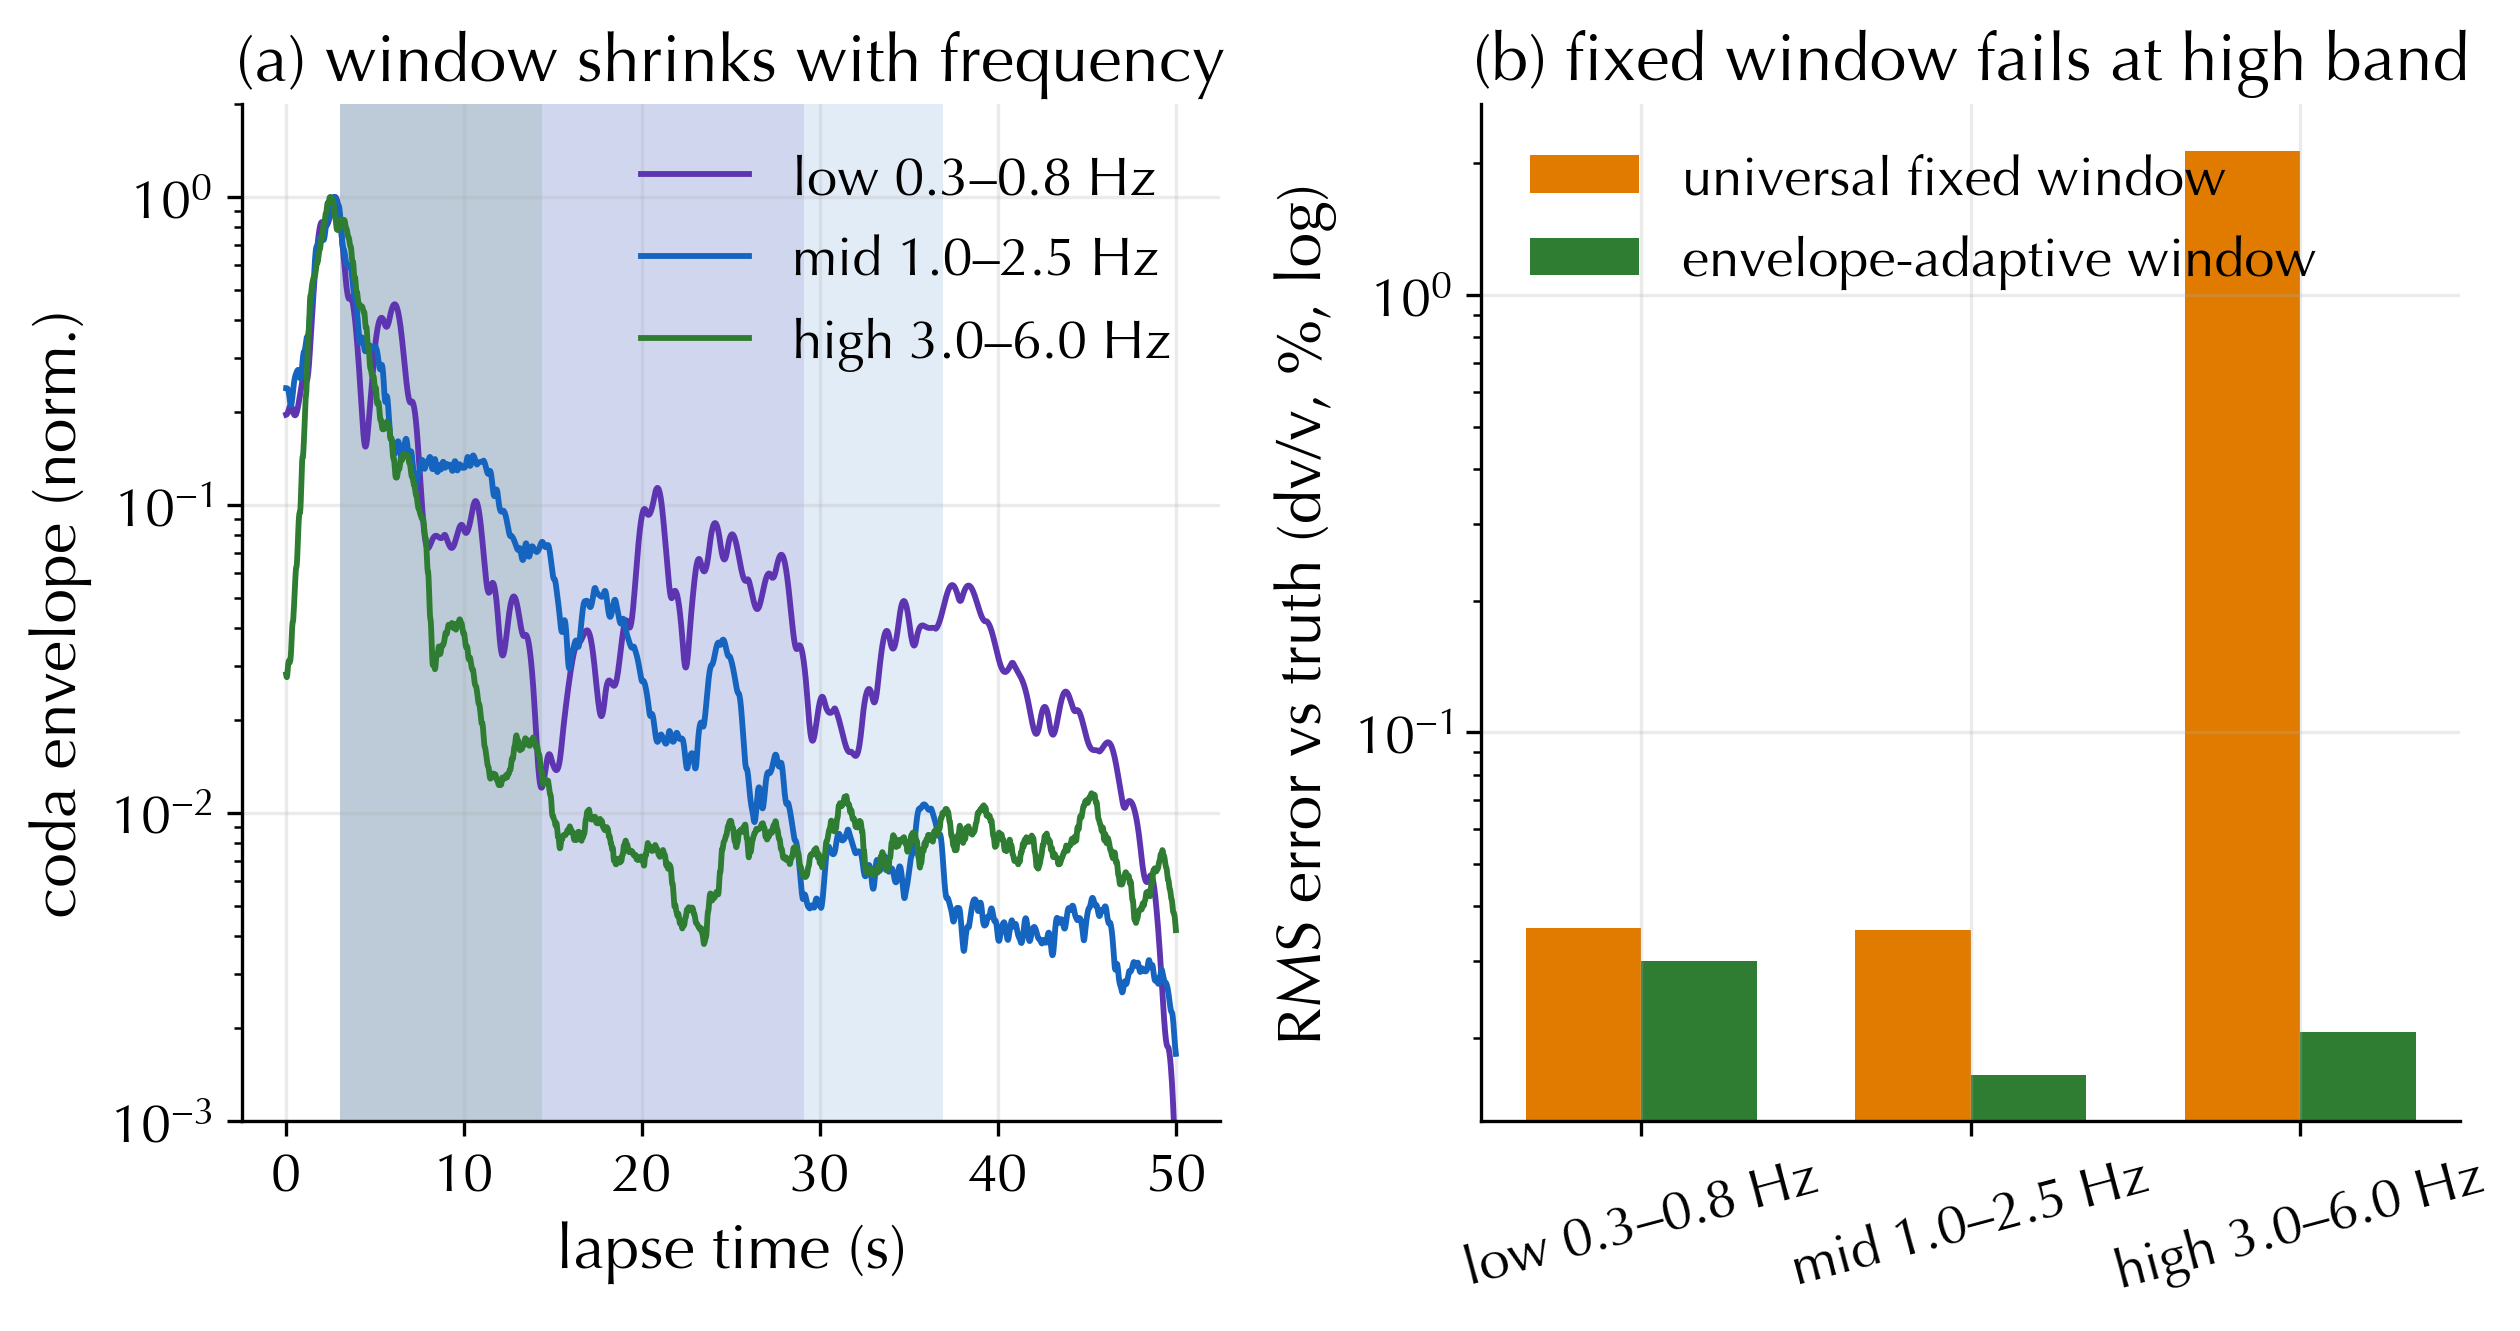
\includegraphics[width=\textwidth]{demo_15_window_envelope.png}
  \caption{Coda window / frequency-band covariation. (a) Smoothed coda
  envelopes at three bands (log scale), shaded by each band's
  envelope-detected window --- shrinking automatically at higher frequency.
  (b) RMS error against the known truth for a single universal fixed window
  versus each band's own envelope-derived window: comparable at low
  frequency, $\sim\!104\times$ better at high frequency.}
  \label{fig:window-envelope}
\end{figure}

\subsection{Causal and acausal branches}\label{sec:branches}

In a symmetric cross-correlation, both sides of the coda (positive or
negative lags) should exhibit the same \dvv. Due to the directionality
of the wavefield recorded at the two stations, the correlated wavefield
in the coda may differ \citep{Stehly2006}. While the interpretation of
such coda in terms of Earth's structure effect is difficult
\citep{Snieder2002}, the stability of the wavefield excited in the coda
is the main requirement for stable \dvv~measurements
\citep{Hadziioannou2009}. Given the challenge in interpreting both sides
independently, researchers typically measure \dvv~on each lag and then
report its average \citep{Kidiwela2026}. The causal (positive-lag) and
acausal (negative-lag) branches sample opposite-direction paths with
different source-side illumination, and in a 3D medium their sensitivity
kernels sample partly different volumes, so the two can report genuinely
different \dvv~without either being wrong. Two regimes bound the choice
(Fig.~\ref{fig:branches}). When a change is \emph{localized} to the
volume one branch samples, symmetrizing or averaging the branches ---
the common default --- dilutes it toward zero, while the branch that
carries the change recovers it (Fig.~\ref{fig:branches}a); here
preferring the branch of greatest change is a researcher's judgement.
When instead both branches share the \emph{same} change, their
difference is measurement noise, and selecting the branch of greatest
change over-reports it --- a max-of-two-estimators selection bias that
grows as SNR falls (Fig.~\ref{fig:branches}b). Choosing the branch of
greatest change after seeing the data is therefore a selection rule that
Fig.~\ref{fig:branches}b shows to be biased, and the coherence of each
branch is estimated from the same observations, so selecting on
coherence reduces but does not remove that bias. The rule we adopt is
fixed before the data are seen: measure both branches and report both;
combine them by their mean unless independent physical information
(source-side illumination, a change known to be confined to one side)
designates a branch beforehand; and carry the between-branch difference
as an explicit term of the measurement covariance \(C_d\)
(Section~\ref{sec:bayes}) rather than discarding it by averaging.

\begin{figure}
  \centering
  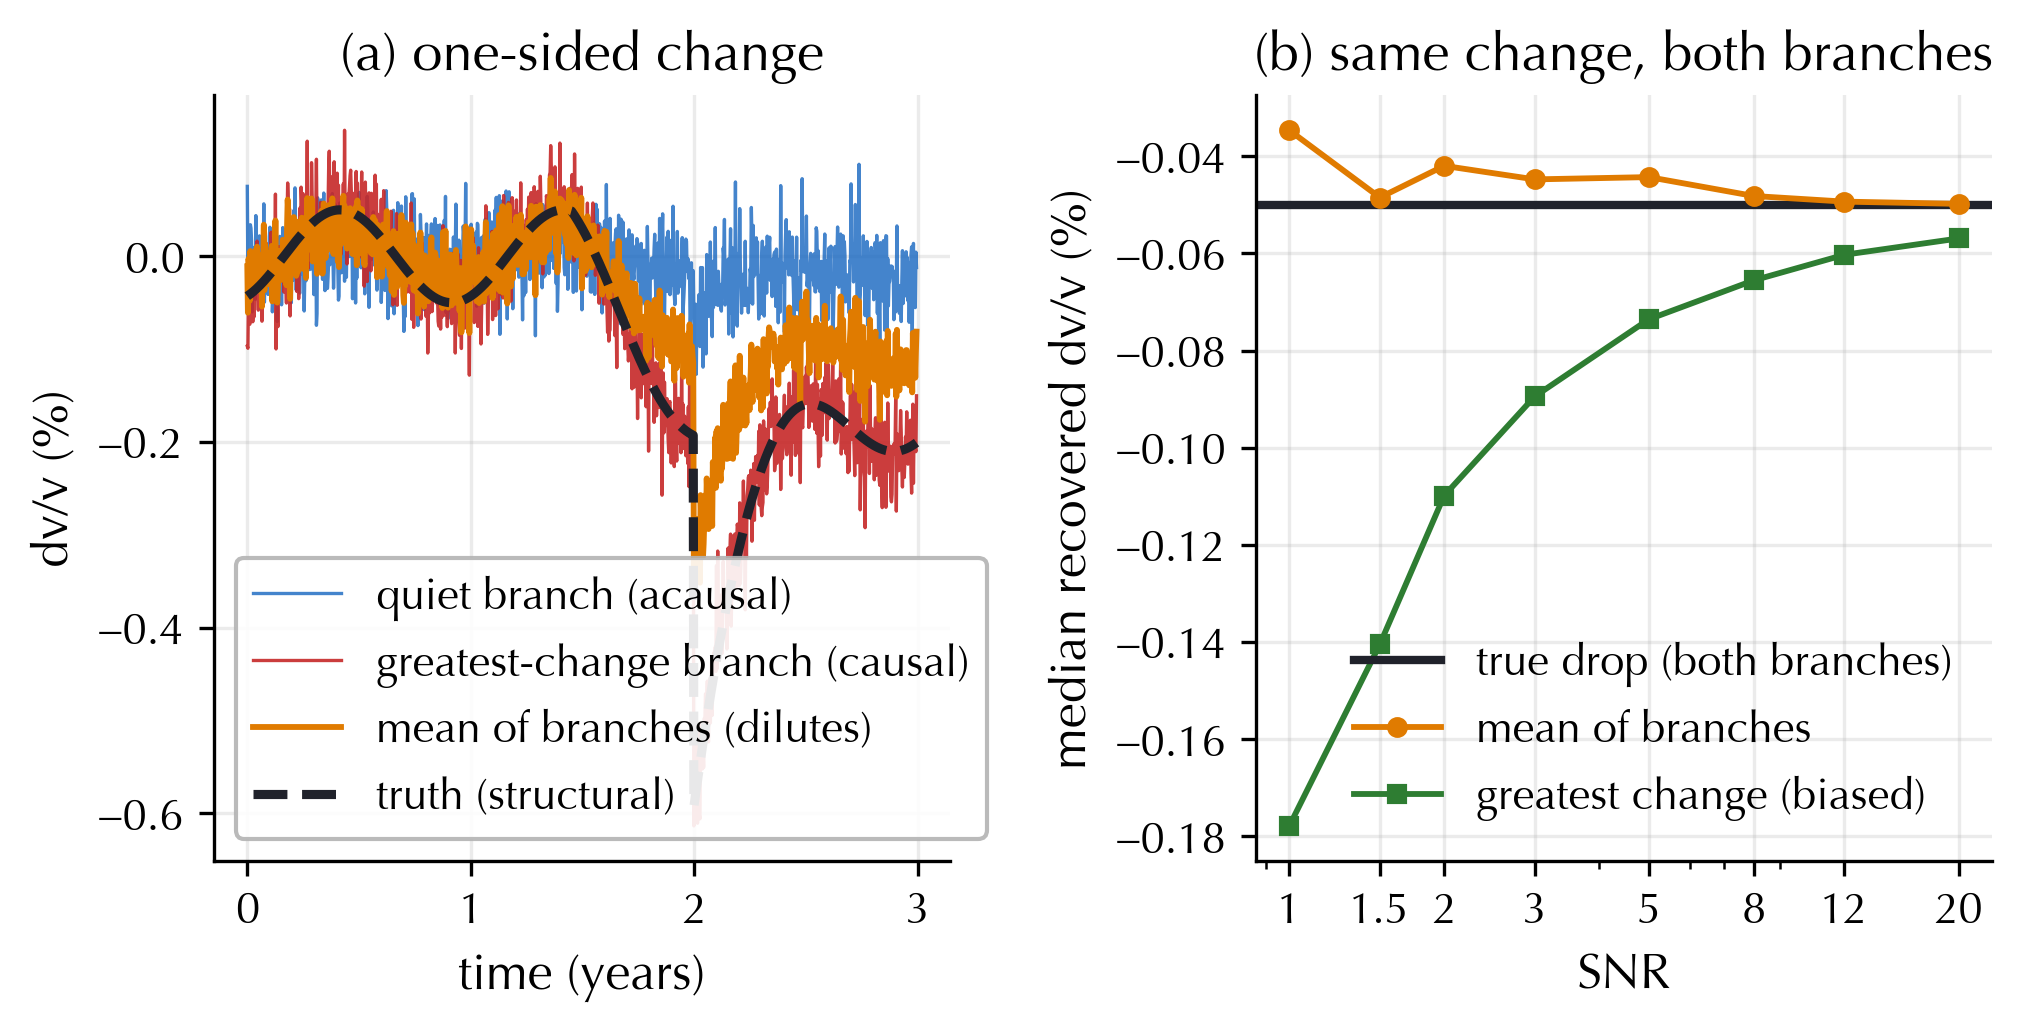
\includegraphics[width=\textwidth]{demo_13_branch_asymmetry.png}
  \caption{Combining the causal and acausal branches. (a) A change localized to
  the volume the causal branch samples: averaging the branches dilutes it to
  about half, while the branch carrying it recovers the truth. (b) The same
  change on both branches: selecting the branch of greatest change over-reports
  the drop, worsening as SNR falls (a selection bias), while the branch mean
  stays unbiased.}
  \label{fig:branches}
\end{figure}

\subsection{\texorpdfstring{Choices that create spurious
\texorpdfstring{\dvv}{dv/v}}{Choices that create spurious }}\label{sec:artifacts}

Some choices may create spurious signal. A station clock error delays
the whole correlation by a lapse-independent shift, producing an
apparent \dvv~that appears with opposite sign on the causal and acausal
branches; measuring the two branches separately is the diagnostic
(Fig.~\ref{fig:artifacts}a). Seasonally varying noise sources warp the
low-SNR late coda, so a late measurement window reports a coherent
spurious \emph{seasonal} \dvv~many times the real signal while an
earlier window stays clean \citep[the waveform-level version
of][]{Zhan2013} (Fig.~\ref{fig:artifacts}b).

Biases from spurious arrivals could be quantified but mostly we should
decontaminate our workflow from these artefacts or not interpret the
results.

\begin{figure}
  \centering
  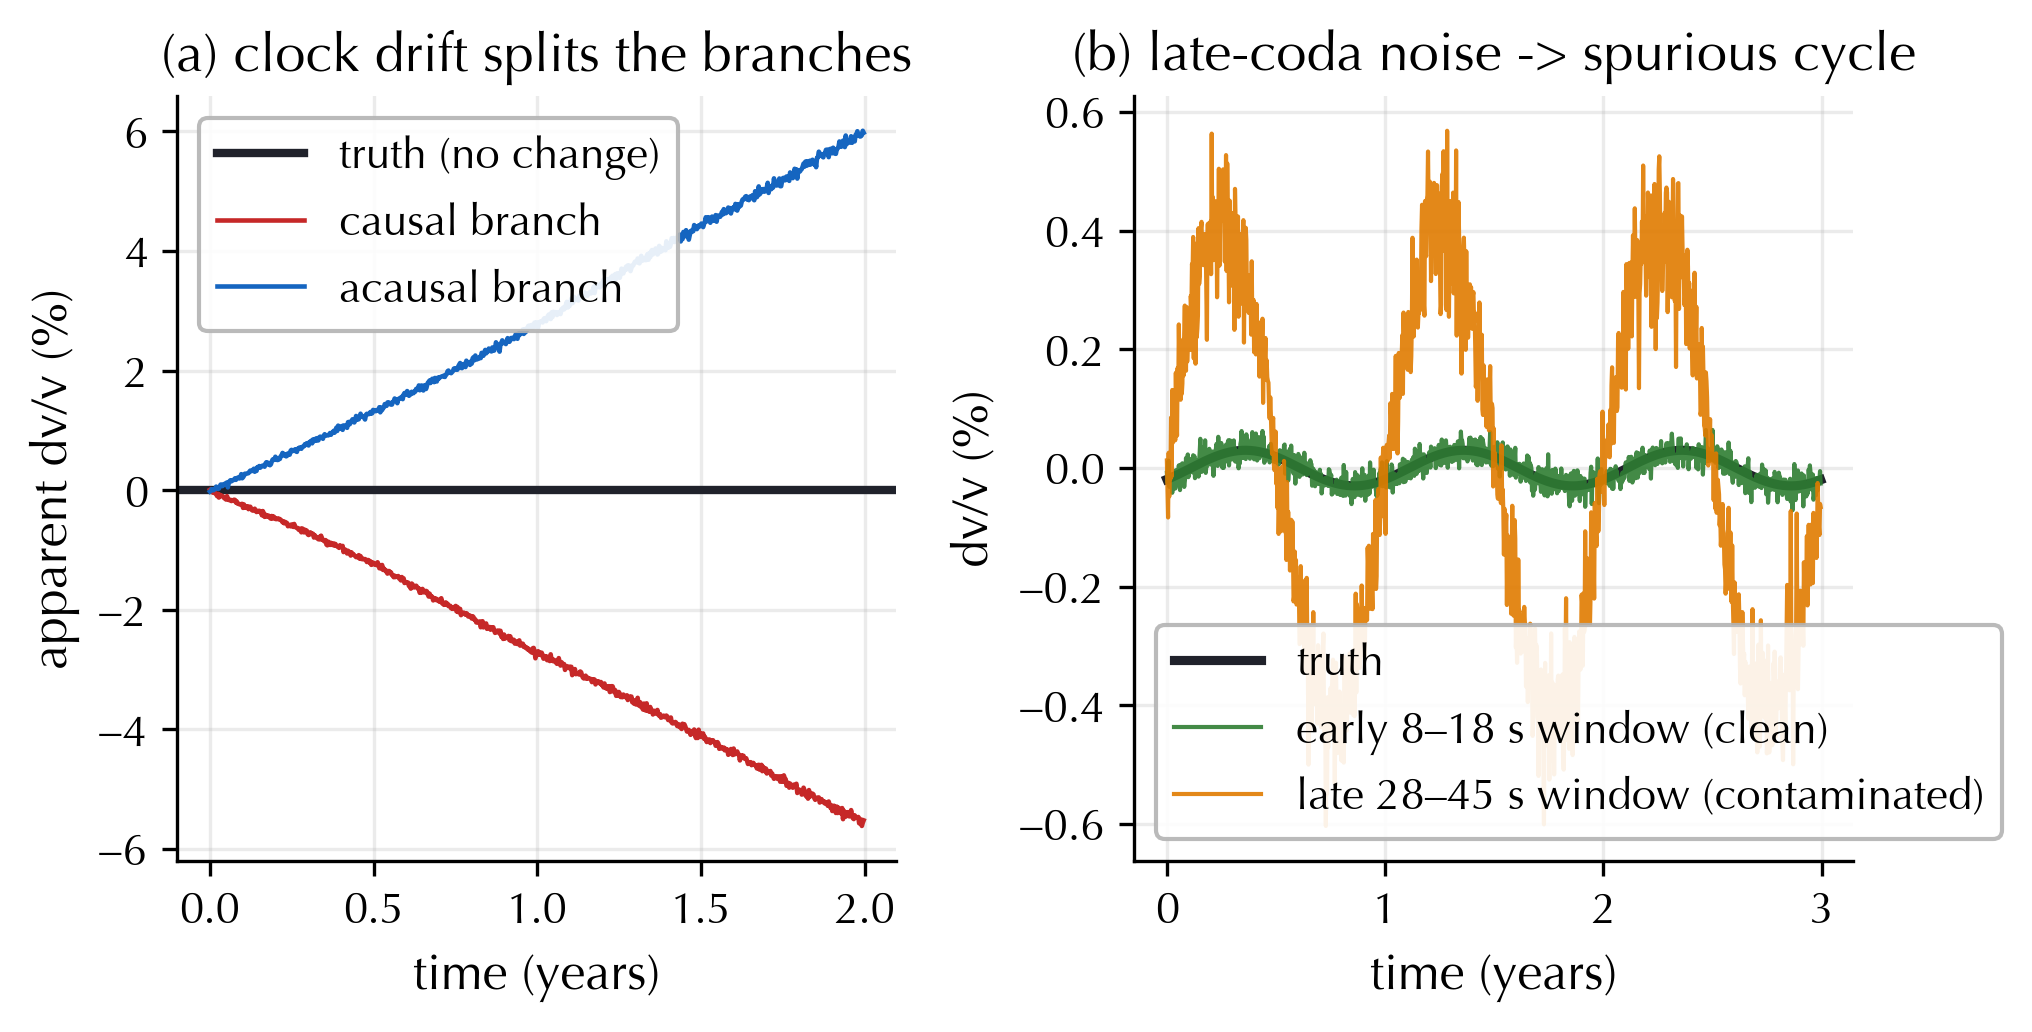
\includegraphics[width=\textwidth]{demo_8_artifacts.png}
  \caption{Deviations that create spurious \dvv. (a) A clock drift splits the causal
  and acausal branches with opposite sign. (b) Seasonal late-coda noise injects a
  spurious seasonal \dvv\ into a late window but not an early one.}
  \label{fig:artifacts}
\end{figure}

Taken together, the choices compound. We make this concrete in
Section~\ref{sec:multiverse} by running the full \emph{multiverse} of
best-practice and deviation choices on one synthetic dataset and ranking
each by the bias and the error-bar change it induces.

\section{The combined impact of processing
choices}\label{sec:multiverse}

The scenario is a single representative station pair monitoring a
shallow volcanic edifice, in the style of the permanent broadband
deployments used at effusive/dome volcanoes such as Piton de la
Fournaise \citep{Brenguier2008}: a coda band matched to shallow depths
(0.4--1.0\(\,\)Hz), a coda window past the direct arrival
(10--30\(\,\)s), and daily correlations sampled every 3 days over 2.5
years at a per-day correlation-coefficient SNR of 7, typical of a
continuously operating station. The synthetic ground truth combines an
annual seasonal \dvv~cycle (as from near-surface
thermoelastic/hydrologic effects), a slow pre-eruptive inflation ramp,
and a sharp co-eruptive velocity drop with partial recovery. This
single-pair scenario isolates the measurement-step choices from the
network-aggregation choices already covered in
Sections~\ref{sec:aggregation}--\ref{sec:uncertainty}.

The previous sections only identified single choices, but the overall
research workflow involves them all. We now estimate the combined
effects of these parametric choices. Starting from a single
\textbf{best-practice baseline} (trace stretching, a band matched to the
target depth, a coda window well past the direct arrival, a 10-day
stack, a long stable reference, coherence gating; the cross-cutting
rules of \citeauthor{Brenguier2014}
\citetext{\citeyear{Brenguier2014}; \citealp{Weaver2011}; \citealp{Clarke2011}}
as distilled in our survey), we change one parameter at a time to a
deviation from best practice documented in the literature and measure
the resulting error against the known truth (Fig.~\ref{fig:deviations}).
The ranking is unambiguous: relative to a best-practice RMS error of
\(\sim\!0.03\,\%\), the two-dimensionally-unwrapped WCS estimator is
catastrophic here (\(\sim\!50\times\) worse), a wrapped-phase MWCS
inflates the error by roughly an order of magnitude
(\(\sim\!12\times\)), and DTW by \(\sim\!6\times\); among the
non-estimator choices the uncumulated trailing reference is worst
(\(\sim\!5\times\), and most distorts the recovered drop; it is an
ablation of re-baselining without trend reconstruction, not a surveyed
workflow, Section~\ref{sec:param_ref}), while stack length, coda window
and frequency band deviations change the error by factors between
\(0.7\) and \(2.5\). Two of them score below the baseline: the
\(0.8\)--\(2\) Hz band (\(0.022\,\%\)) and the \(4\)--\(14\) s window
(\(0.027\,\%\)) against the baseline's \(0.032\,\%\), so the
best-practice baseline is not the optimum of this scenario. Turning the
coherence gate off leaves the error unchanged here. The joint-inversion
reference stays closest to the fixed-reference baseline among the
reference-scheme deviations.

\begin{figure}
  \centering
  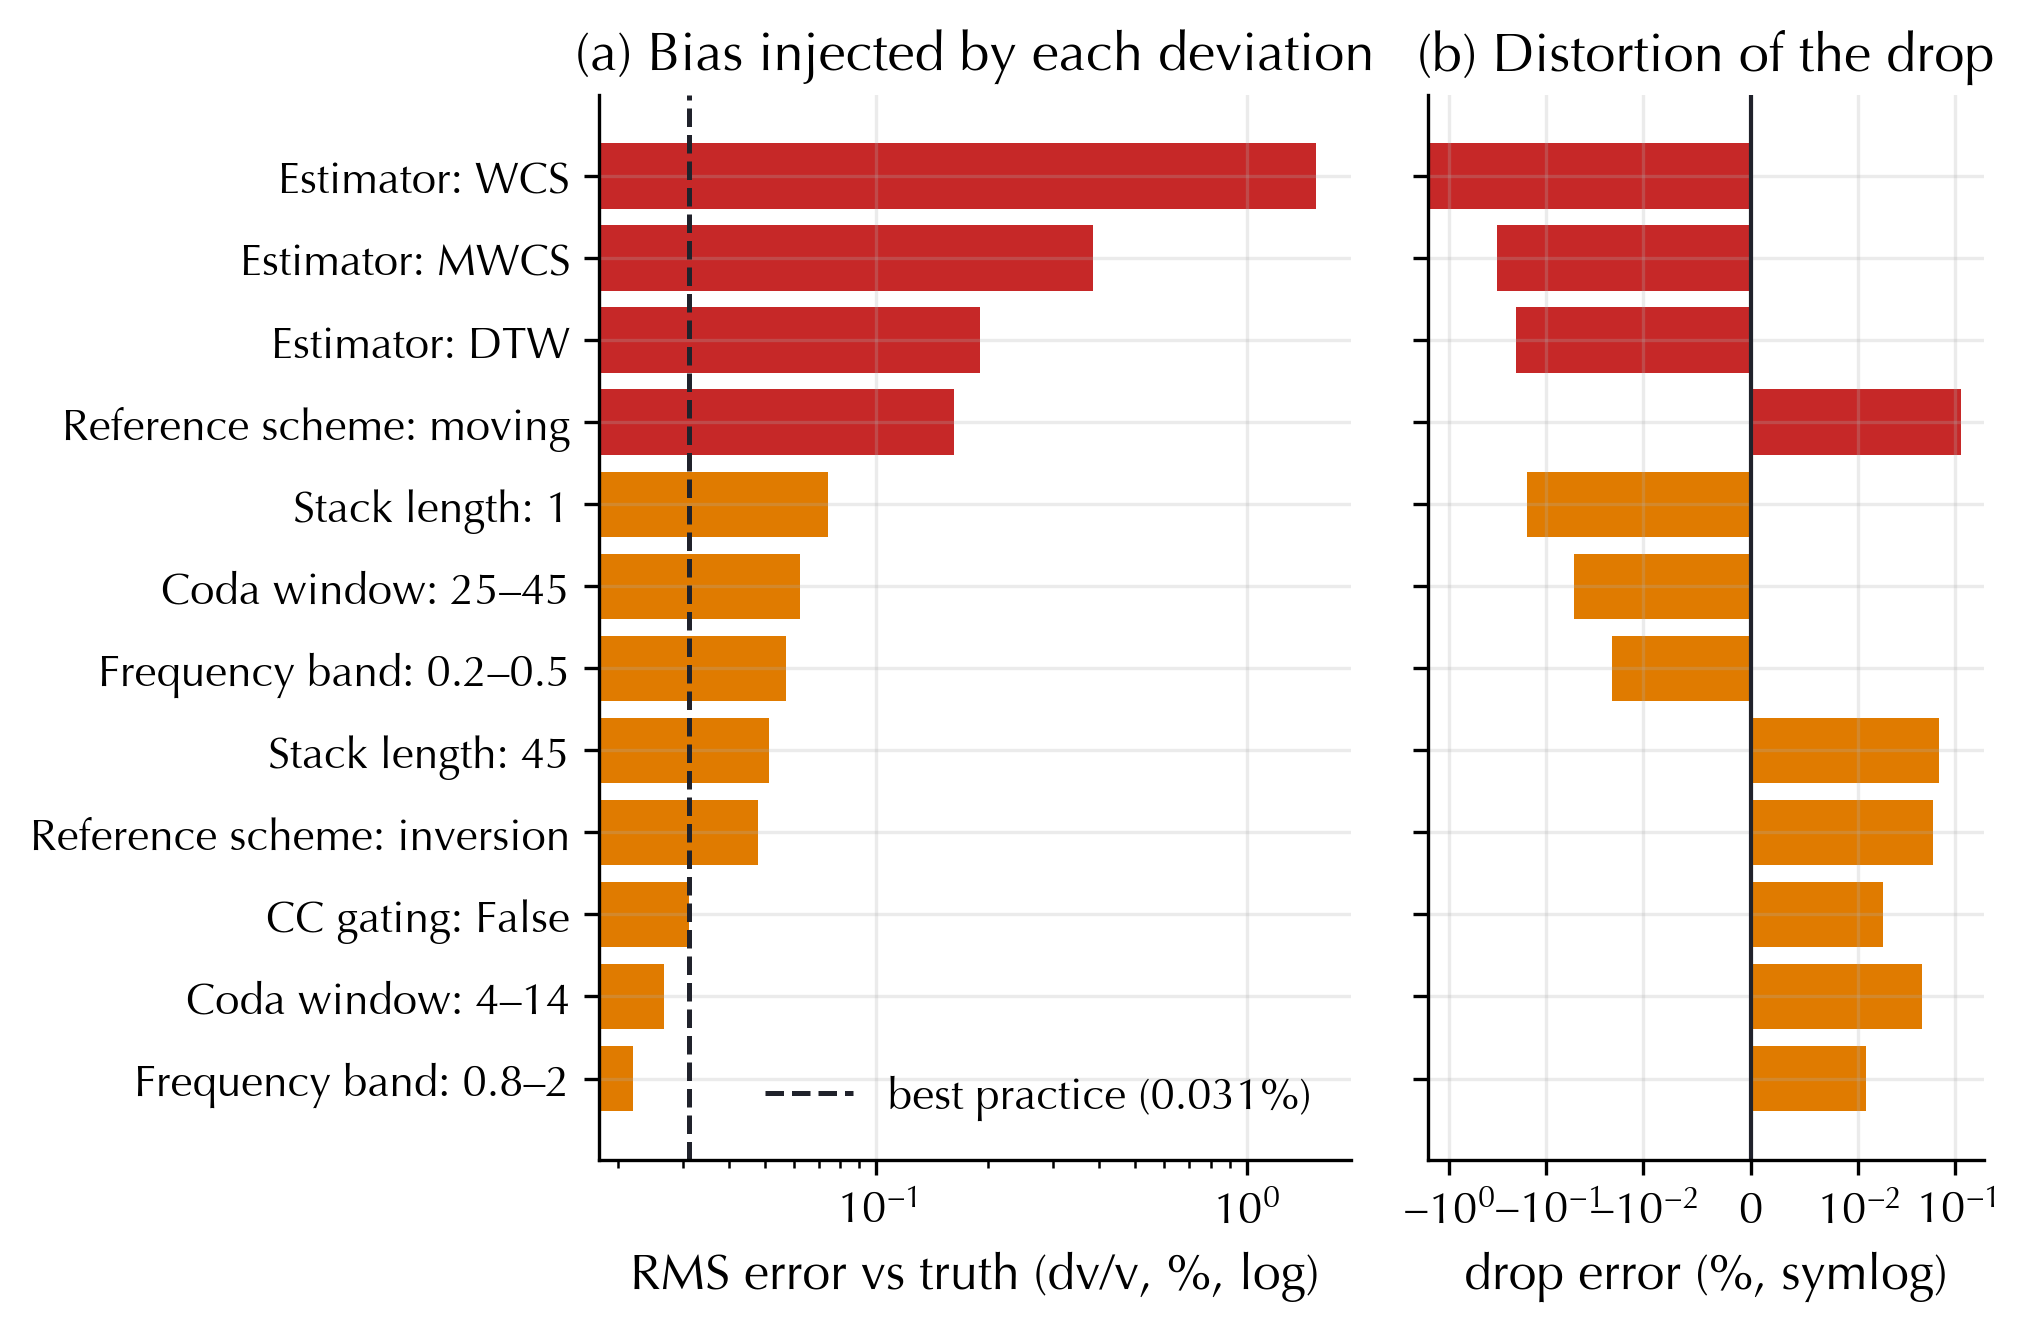
\includegraphics[width=\textwidth]{demo_10_deviations.png}
  \caption{One-at-a-time deviations from a best-practice baseline, ranked by
  their RMS error against the truth (a, log scale; RMS mixes bias and
  scatter) and by how they distort the recovered co-eruptive drop (b,
  symlog). Bars are coloured red when the error exceeds three times the
  baseline (dashed line). "Uncumulated trailing" is the moving reference
  without trend reconstruction of Section\ \ref{sec:param_ref}.}
  \label{fig:deviations}
\end{figure}

We test the compounding effects of these choices through 108 reasonable
workflows selecting three estimators, two frequency bands, three coda
windows, three stacking lengths and two reference schemes on a synthetic
``volcano'' dv/v time series that includes a seasonal oscillation, a
slow pre-eruptive inflation ramp, and a sharp co-eruptive drop with
partial exponential recovery (Fig.~\ref{fig:multiverse}a). The per-day
standard deviation across the 108 pipelines varies by a factor of
\(\sim\!4\)--5 over the time series (from \(\sim\!0.4\,\%\) to
\(\sim\!1.7\,\%\)), and is widest exactly at the sharp co-eruptive drop;
the RMS error against the known truth spans over two orders of magnitude
across pipelines (\(\sim\!0.02\)--\(2.8\,\%\)).

Attributing the variance of the outcome to each axis with a first-order
(main-effect) sensitivity index (Fig.~\ref{fig:multiverse}b) shows that,
for this dataset, the \textbf{coda window} controls the RMS error most,
with the estimator second and the stack length third; for the recovered
drop amplitude the order changes to \textbf{stack length} first, window
second, and estimator third. The first-order indices sum to well under
one in both cases (\(\sim\!0.66\) for RMS, \(\sim\!0.63\) for the drop),
so a large part of the spread is \emph{interaction} between choices
compounding. The appropriate object is therefore not a single curve but
a distribution of \dvv~over the processing choices.

\begin{figure}
  \centering
  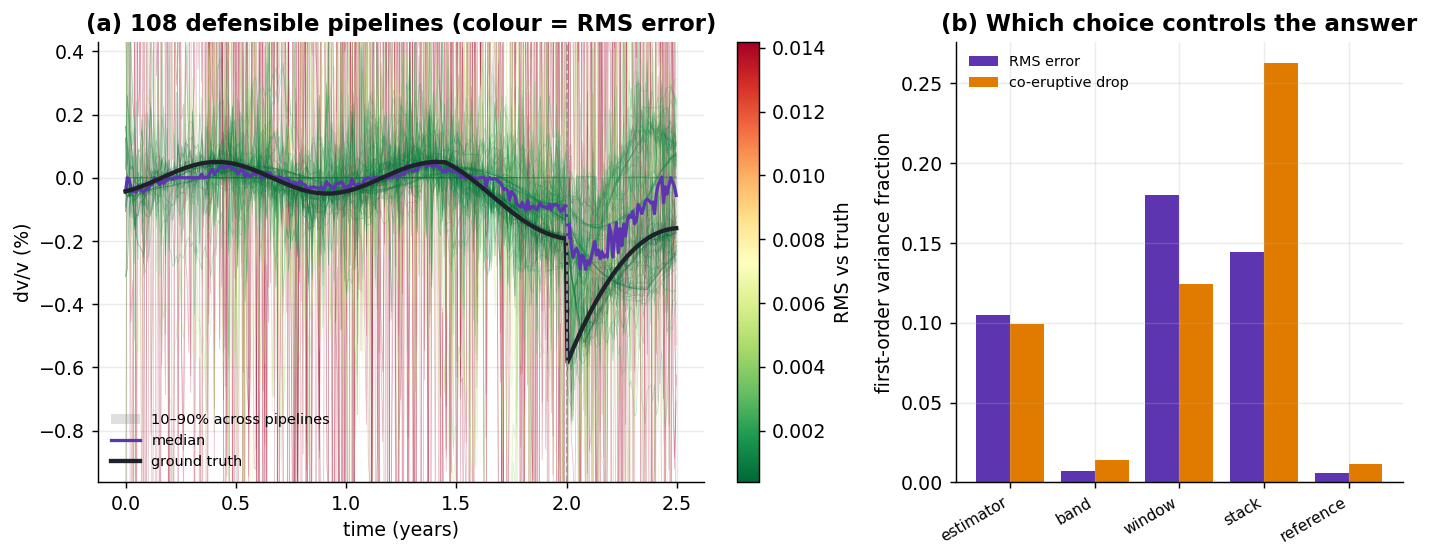
\includegraphics[width=\textwidth]{demo_11_multiverse.png}
  \caption{The full multiverse. (a) 108 reasonable pipelines on one dataset,
  each coloured by its RMS error against the truth (a fraction of velocity) on
  a colourblind-safe scale (bright accurate, dark biased), with the median
  across pipelines (purple) and the truth (black); the axis is clipped at
  $\pm0.8\,\%$, and the number of pipelines that leave it and the extent of
  the 10--90\% inter-pipeline band, which exceeds the axis range, are printed
  on the panel. (b) First-order variance attribution of the RMS error and of
  the recovered drop to each processing axis.}
  \label{fig:multiverse}
\end{figure}

Table~\ref{tab:bp-measure} summarizes this into the measurement-step
best practice and the documented deviation for each choice, with the
consequence the synthetic makes concrete. The baseline and deviation
sets are the ones our survey extracts from the literature (the
cross-cutting rules of \citeauthor{Snieder2002}
\citetext{\citeyear{Snieder2002}; \citealp{Clarke2011}; \citealp{Weaver2011}; \citealp{Brenguier2014}; \citealp{Wang2017}; \citealp{Obermann2019}})
and are implemented in codameter.

\begin{table}
\footnotesize
\caption{Measurement step: best practice versus the common deviation and its
consequence. Rows are the axes swept in Fig.~\ref{fig:multiverse}; the sets
follow the literature survey (Appendix~\ref{app:survey}).}
\label{tab:bp-measure}
\begin{tabularx}{\textwidth}{@{}>{\raggedright\arraybackslash}p{2.5cm} L L L@{}}
\toprule
\textbf{Choice} & \textbf{Best practice} & \textbf{Common deviation} &
\textbf{Consequence} \\
\midrule
Estimator & Stretching family (TS/WTS/WCC), robust at low SNR and large \dvv\ \citep{Mikesell2015,Yuan2021} & Wrapped-phase MWCS \citep{Clarke2011} without 2-D
unwrapping \citep{Mao2020} & Cycle-skips at large \dvv; error inflated
$\sim\!10\times$ or catastrophic \\ \hline
Frequency band & Matched to the target depth: $\sim\!0.1$--2\,Hz (volcano, crust),
2--4\,Hz (aquifer), 4--12\,Hz (shallow damage) \citep{Obermann2013,Obermann2016} &
Off-target or a single wide band & Mixes depths; here mostly sets precision \\ \hline
Coda window & Lapse window past the direct arrival, scaled with the band:
$\sim\!5$--30\,s (crustal) up to $\sim\!100$\,s (station pairs) \citep{Obermann2013} &
Fixed late window reused across bands & Measures noise at high $f$; bias and
inflated $\sigma$ \\ \hline
Stack length & Short enough to resolve the transient ($\sim\!10$\,d), on a long,
stable reference span \citep{Wang2017} & Over-long stack ($\sim\!45$\,d) & Smears and
delays a step; distorts the recovered drop \\ \hline
Reference & Long fixed stack or all-to-all joint inversion
\citep{Brenguier2014,Wang2017} & Uncumulated trailing reference (an ablation:
published moving-reference workflows cumulate or stitch,
Section~\ref{sec:param_ref}) & Erases slow trends \\ \hline
Coherence gating & Discard low-coherence epochs (CC / SNR threshold)
\citep{Clarke2011} & No gating & Keeps corrupted epochs; changes the effective $N$ \\ \hline
Uncertainty definition & State it explicitly: within-measurement
\citep{Weaver2011,Clarke2011} / SE / SD & Left unstated & Factor $\sqrt{N}$
ambiguity in significance (Fig.~\ref{fig:uncertainty}) \\
\bottomrule
\end{tabularx}
\end{table}

Running this many pipelines is only practical if each one is cheap.
Testing codameter against a larger, multi-year deployment surfaced real
bottlenecks in the per-day estimator loop, which we removed with three
vectorized fast paths: a trailing stack built from a difference of
cumulative sums instead of a per-day mean (roughly \(2\times\) at a
45-day stack length), a vectorized moving-reference stretching estimator
that computes the stretch-interpolation weights once per trial epsilon
instead of once per day (roughly \(3\times\) on a 3-year synthetic),
and, for ensembles that share a band, a single shared band-pass instead
of one per pipeline member (roughly \(3\times\) on a 5-member ensemble).
All three reproduce the loops they replace to within \(10^{-15}\) in
\dvv~(regression-tested at \(\mathrm{atol}=10^{-12}\)); the reported
ratios are wall-clock, vary with system load, and should be read as
``roughly \(N\times\),'' not exact.

\section{A Bayesian measurement model and its data
covariance}\label{sec:bayes}

If the processing choice controls the answer, the principled response is
not to select a single pipeline but to treat the choice as a
\textbf{nuisance parameter} with a prior and assess its influence. We
explore a Bayesian hierarchical model for the \dvv~\emph{measurement},
conditional on a specified pipeline menu. For configuration \(k\) drawn
from a prior over reasonable pipelines we obtain a measured series
\(m_k(t)\) with a coherence-limited within-method floor \(\sigma_k(t)\)
\citep{Weaver2011, Clarke2011}, and posit \begin{equation}
m_k(t) = \mu(t) + \beta_k + \varepsilon_k(t), \qquad
\beta_k\sim\mathcal N(0,\tau^2),\quad
\varepsilon_k(t)\sim\mathcal N\!\big(0,\,s^2\sigma_k(t)^2\big),
\label{eq:bayes}
\end{equation} The likelihood treats residuals as conditionally
independent across configurations and epochs. Shared input waveforms do
not ensure this assumption. Fitting all member outputs jointly is not
the same operation as marginalising a discrete mixture of alternative
pipelines. The posterior is therefore conditional on this working
likelihood. We use a second-difference smoothness prior of precision
\(\lambda\) on the latent true series \(\mu(t)\), built on the physical
time grid so that a gap in the record is a gap in the prior. Here
\(\beta_k\) is configuration \(k\)'s constant offset (the systematic
offset between, say, MWCS and stretching), \(\tau\) its scale across the
ensemble, and \(s\) rescales the coherence floor of eq.~\ref{eq:weaver}
so that the data report whether that floor is calibrated. Every
configuration is run through the same pipeline code as the rest of the
paper, so the estimator, band, window, stack length in days, reference
scheme and coherence gate all take effect; an epoch a configuration does
not produce (reference warm-up, a gated coherence) is simply missing and
carries no information. The hyper-priors on \(\tau^2\), \(s^2\) and
\(\lambda\) are conjugate inverse-gamma and gamma distributions whose
scales are small against the data terms. Codameter reports the prior
scale term divided by the conditional posterior rate, evaluated at
posterior means. The ratio is about 0.09 for \(\tau^2\) in the clean
scenario and below 0.01 for \(s^2\) and \(\lambda\)
(Table~\ref{tab:calibration}). This diagnostic does not measure the
total influence of the prior or establish sampler convergence. A
conjugate Gibbs sampler, implemented in codameter with no external
sampler dependency and with a banded solve for the smoothness update,
returns the joint posterior.

The model yields two distinct objects, and conflating them is a common
error (Fig.~\ref{fig:bayes}; Table~\ref{tab:estimands}). The posterior
of \(\mu\) is the precision of the \emph{combined} estimate: it is tight
and shrinks with ensemble size under the working likelihood. Separately,
we construct a candidate \textbf{single-member error covariance}
\begin{equation}
C_d(t,t') = \underbrace{D R D}_{\text{calibrated floor}\,\oplus\,\text{excess spread},\ \text{temporally correlated}}
\;+\; \underbrace{\tau^2\,\mathbf{1}\mathbf{1}^\top}_{\text{common mode}},
\qquad D=\operatorname{diag}\!\big(\sigma_{\mathrm{tot}}(t)\big),
\label{eq:cd}
\end{equation} with
\(\sigma_{\mathrm{tot}}^2(t) = s^2\,\overline{\sigma_k^2(t)} +
\max\!\big[\operatorname{Var}_k(m_k(t)-\beta_k) - s^2\,\overline{\sigma_k^2(t)},\,0\big]\),
the calibrated floor plus whatever spread across configurations exceeds
it (so that the floor is not counted twice), and
\(R_{ij}=e^{-|t_i-t_j|/L}\) for a correlation length \(L\) estimated
from the ensemble residuals. \(C_d\) is constructed from the fitted
model, not sampled. It targets the error of one measurement drawn from
the ensemble, not of \(\mu\). The between-configuration offset scale
\(\tau\) does not identify an error shared by all configurations.
Pointwise coverage tests only the diagonal scale; it does not validate
\(R\) or the rank-one term. A downstream inversion needs the error
covariance of its actual input estimate. Neither using this \(C_d\) for
the ensemble mean nor interpreting its time axes as frequency-band axes
is justified here.

Two properties of the fit deserve to be stated plainly. First,
\(s\approx 12\) on this synthetic: the residual scatter of the members
about the ensemble mean is an order of magnitude above the coherence
floor of eq.~\ref{eq:weaver}, which treats the reference as noise-free
and knows nothing of the estimator. The floor is a lower bound, and the
rescale is what makes it usable. Second, once \(s\) is fitted on those
residuals, the calibrated floor absorbs nearly all of the
between-configuration spread, and the excess term of eq.~\ref{eq:cd} is
non-zero only at the epochs where the configurations disagree more than
they usually do (Fig.~\ref{fig:bayes}c). The assumed temporal
correlation (\(L\approx 39\) days on the realisation shown, 30 days on
average over the 200 realisations of Table~\ref{tab:calibration}, at a
4-day cadence) and the common-mode term collapse the effective number of
independent epochs from 229 to a few tens.

Whether these intervals mean what they say is a question one realisation
cannot answer, so we repeat the whole measurement on independent
realisations of the same scenario (Table~\ref{tab:calibration}; the
driver is \texttt{codameter.calibration}). Three coverages answer three
different questions. The fraction of member epochs whose error against
the truth lies within \(1.96\,\sigma_{C_d}\) is 0.956 on 200
realisations, within the margin of \(\pm 0.03\) fixed before the run.
This supports the \(95\,\%\) pointwise interval on this scenario, not
calibration of the entire covariance. At the \(68\,\%\) level it covers
0.81 and fails the same margin. One Gaussian scale therefore does not
calibrate both interval levels. The \(95\,\%\) credible band on \(\mu\)
contains the truth at only 0.59 of the epochs: the ensemble mean
inherits the biases its members share (the stacking that rounds the
drop, the estimator biases at low coherence), and no amount of averaging
over configurations removes them, which is what the posterior's
precision cannot know. Comparing \(\mu\) with \(\pm 2\sigma_{C_d}\)
mixes the ensemble mean with a single-member scale and yields nearly
complete coverage here; it does not validate the uncertainty of the
combined estimate. The other two scenarios of
Table~\ref{tab:calibration} inject artefacts that every configuration
sees identically. A station clock drift changes no coverage by more than
0.015 and adds no shared bias (Table~\ref{tab:calibration}), because a
lapse-independent shift appears with opposite signs on the causal and
acausal branches (Section~\ref{sec:artifacts}) and every configuration
in this ensemble measures both branches together, so the drift cancels
in the estimate. What the drift does change is the coherence, which
raises the within-method floor of eq.~\ref{eq:weaver}: the fitted
rescale falls from \(s=11.7\) to \(10.9\) while the median
\(\sigma_{C_d}\) is unchanged (\(0.225\) against \(0.222\,\%\)). The
cancellation is a property of the two-branch measurement, not evidence
that the ensemble could have detected it. A seasonal source effect
confined to the late coda, the waveform-level artefact of
\citet{Zhan2013} (Section~\ref{sec:artifacts}), is the genuine shared
error: it warps the coda every configuration measures, and on that
scenario the credible band covers the truth at only 0.34 of the epochs
and the RMSE of \(\mu\) more than doubles, from 0.067 to \(0.161\,\%\),
while the member-level coverage of \(C_d\) stays at 0.95. That last
number is right for a reason that gives no comfort: the artefact also
inflates the scatter that \(s\) absorbs, so \(C_d\) widens, but its
coherent part biases every member and the ensemble mean together and
leaves no trace in their spread. That is the limit of the method, not a
defect of the fit: an ensemble over processing choices can only reveal
the errors on which its members disagree, and an error shared by every
pipeline (a source change, a contaminated reference, a clock drift
measured on one branch) needs an independent diagnostic, such as the
branch asymmetry of Section~\ref{sec:artifacts}.

\begin{figure}
  \centering
  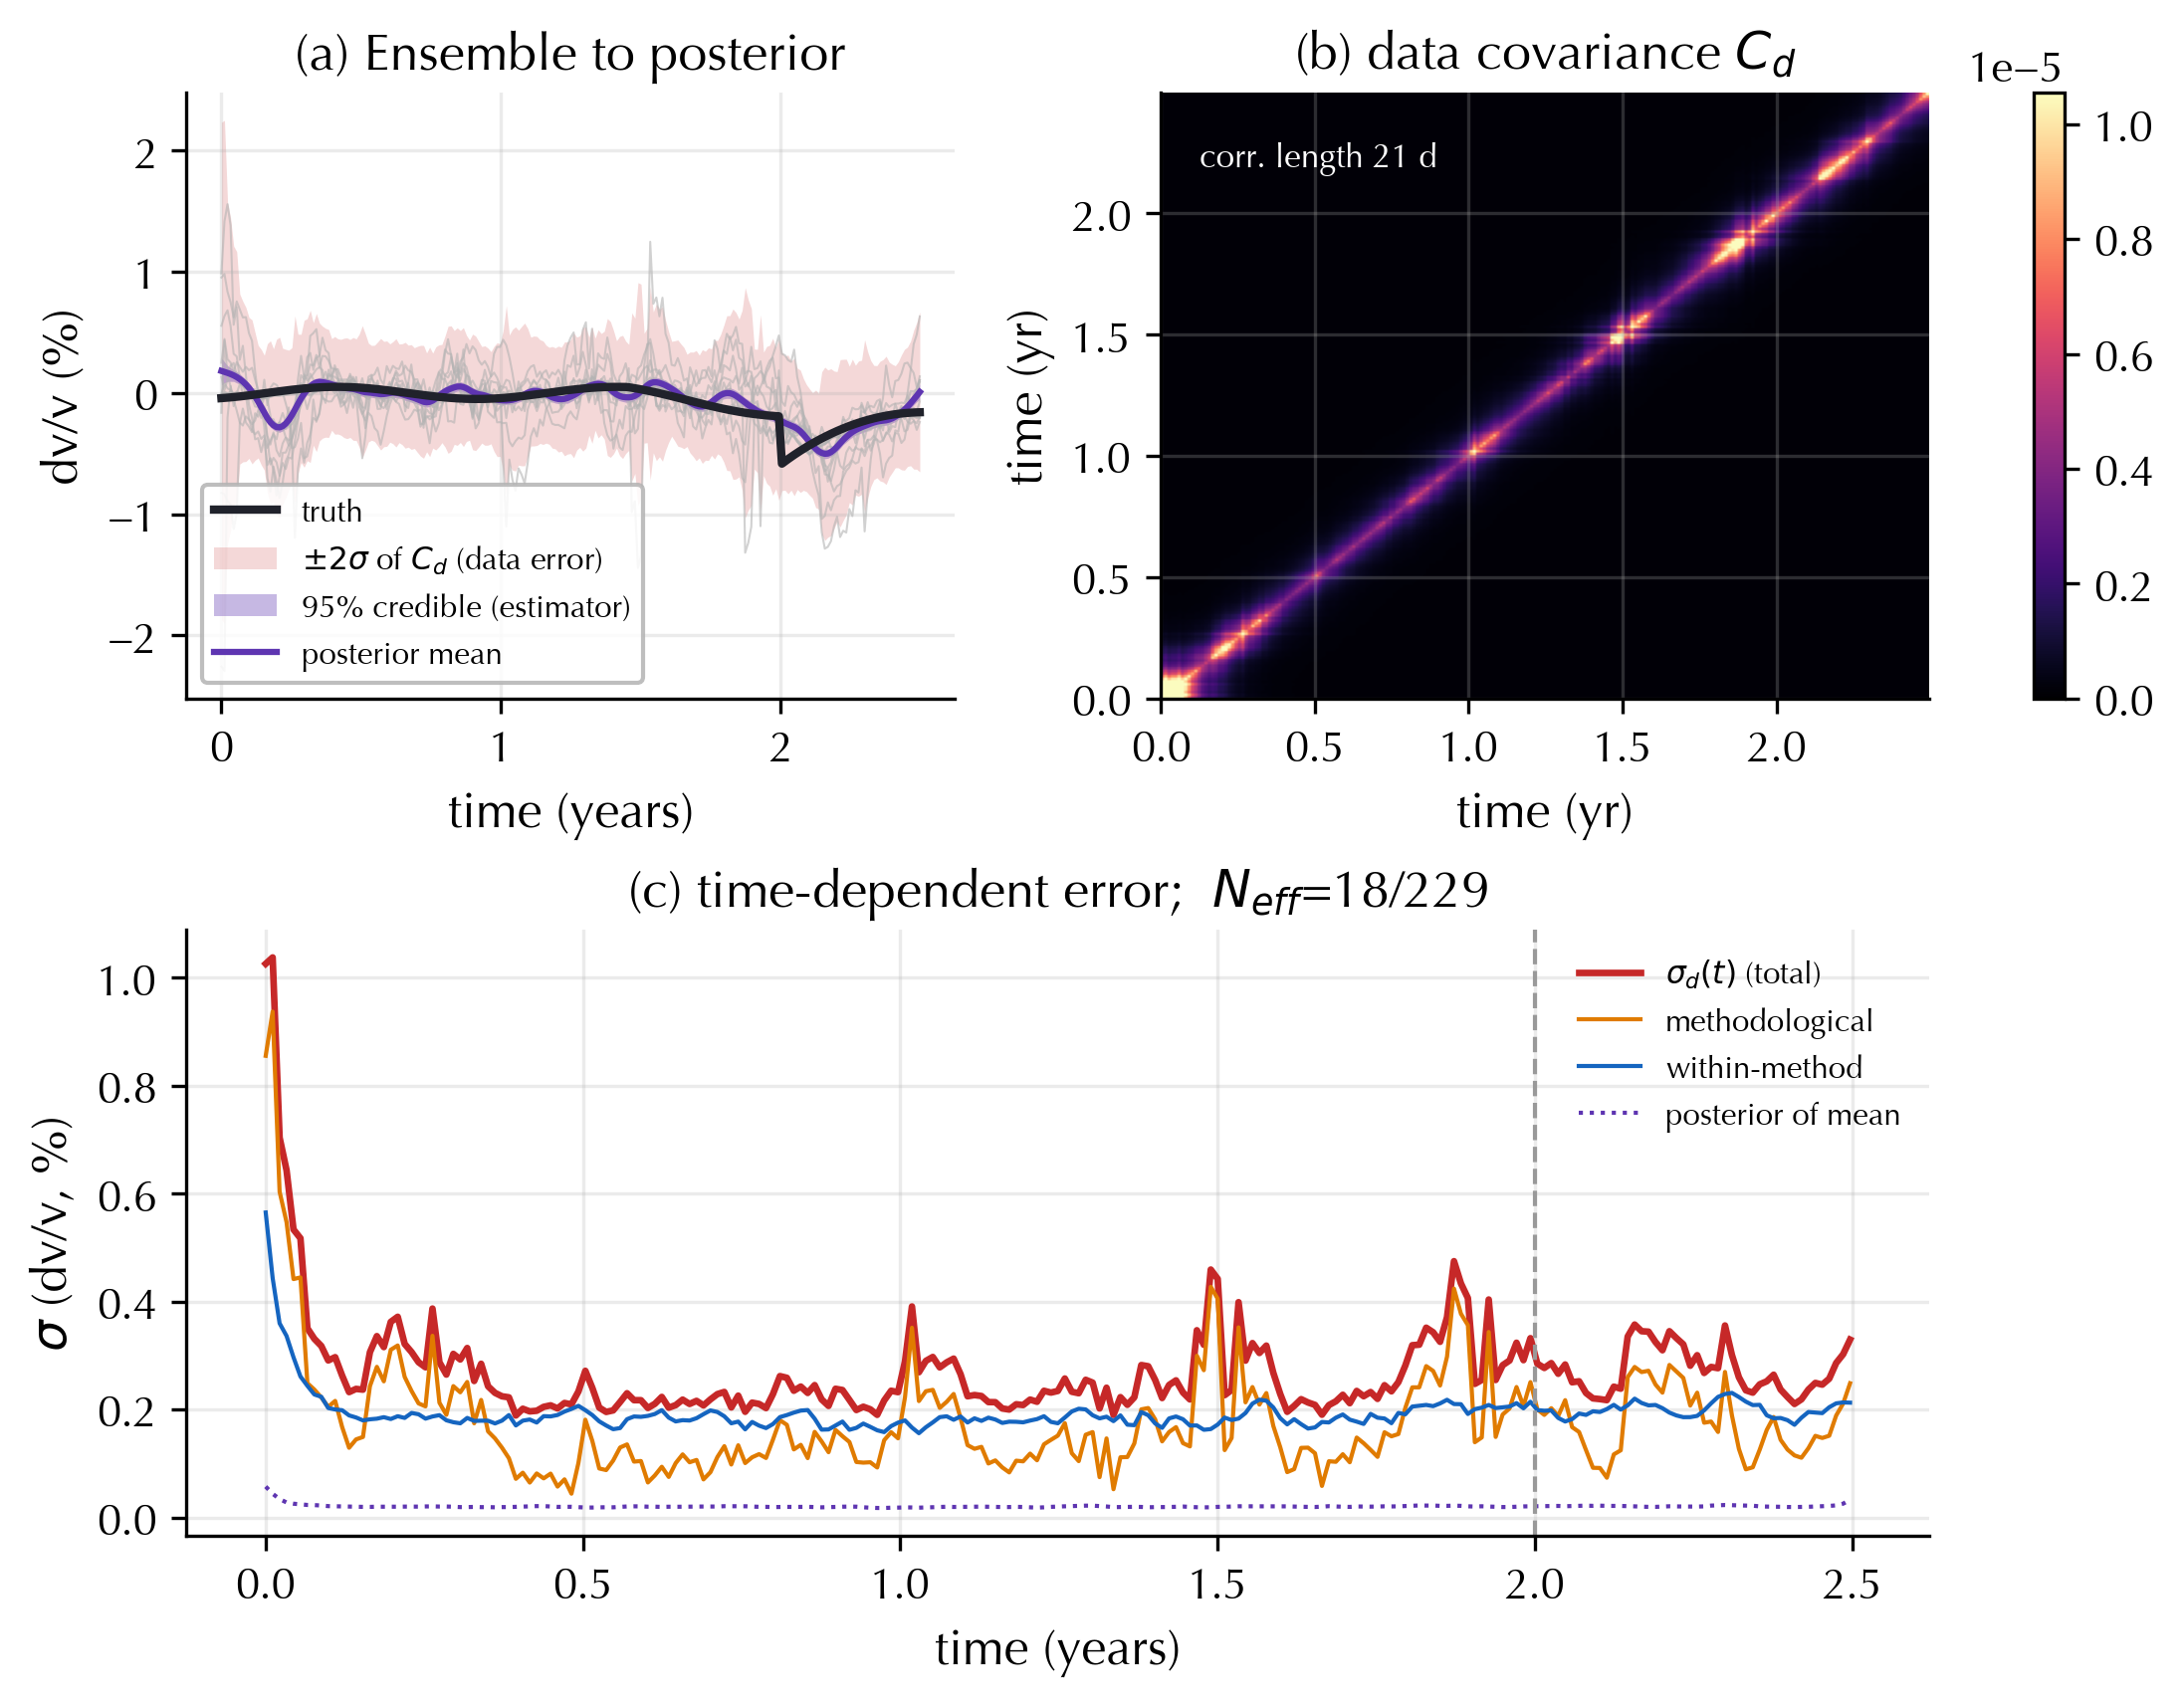
\includegraphics[width=\textwidth]{demo_12_bayes.png}
  \caption{The Bayesian measurement model on one realisation of the volcano
  scenario (12 configurations: three estimators, two bands, two windows, 10-day
  stacks, fixed reference, 4-day cadence). (a) The twelve ensemble members
  (grey) are combined into a posterior mean (purple) with its 95\% credible
  band (purple, narrow) and the $\pm1.96\,\sigma$ band of $C_d$, the
  single-member error (red), which encloses 95\% of member epochs over
  repeated realisations (Table~\ref{tab:calibration}).
  (b) The time-dependent covariance $C_d$, in squared fractional \dvv.
  (c) Its diagonal $\sigma_d(t)$, in percent, split into the rescaled
  within-method floor ($s\,\overline{\sigma_k}$) and the excess
  between-configuration spread, with the posterior standard deviation of the
  mean (dotted); $N_{\mathrm{eff}}$ is the effective number of independent
  epochs implied by $C_d$.}
  \label{fig:bayes}
\end{figure}

\begin{table}
\footnotesize
\caption{Coverage calibration of the Bayesian measurement model over independent synthetic realisations of the volcano scenario (2.5 years, SNR 7, 4-day cadence, 12-member ensemble). Member coverage: fraction of member epochs with $|m_k(t)-\mathrm{truth}(t)|\le z\,\sigma_{C_d}(t)$, the quantity $C_d$ is a covariance of. Posterior: fraction of epochs whose 95\% credible band on $\mu$ contains the truth. $\mu\pm\sigma_{C_d}$: the comparison an earlier draft quoted, which mixes the ensemble mean with a single-measurement scale. Means with standard errors across realisations; $\sigma_{C_d}$, bias and RMSE in percent; prior shares are the fraction of the $\tau^2$ and $\lambda$ posteriors supplied by their hyper-priors. Shared drift: a clock drift of $4\times10^{-5}$\,s/day from 40\% of the record, seen by every configuration. Generated from \texttt{paper/data/calibration/} by \texttt{paper/build\_calibration\_table.py}.}
\label{tab:calibration}
\begin{tabular}{@{}lrrllllrrrrr@{}}
\toprule
Scenario & $n$ & failed & member 68\% & member 95\% & posterior 95\% & $\mu\pm\sigma_{C_d}$ 95\% & med.\ $\sigma_{C_d}$ & bias & RMSE($\mu$) & prior $\tau^2$ & prior $\lambda$ \\
\midrule
clean & 20 & 0 & 0.804 $\pm$ 0.003 & 0.955 $\pm$ 0.001 & 0.593 $\pm$ 0.011 & 1.000 $\pm$ 0.000 & 0.227 $\pm$ 0.002 & -0.017 $\pm$ 0.001 & 0.070 $\pm$ 0.002 & 0.09 $\pm$ 0.03 & 0.00 $\pm$ 0.00 \\
\bottomrule
\end{tabular}
\end{table}


\section{\texorpdfstring{Propagating \dvv~errors at depth
\(\Delta\beta/\beta(z)\)}{Propagating ~errors at depth \textbackslash Delta\textbackslash beta/\textbackslash beta(z)}}\label{sec:depth}

The remaining sections present a framework rather than new synthetics:
they set out how the covariance of Section~\ref{sec:bayes} propagates
down the inference chain, and ground each step in what the monitoring
literature does and does not yet report. The executable stages are in
development in the open codameter package
(Section~\ref{sec:discussion}).

The field has converged on one physical rule for depth --- \emph{depth
is set by the frequency band and the coda lapse time, it is not assumed}
\citep{Obermann2013, Obermann2016} --- and, increasingly, on multi-band
measurement as the means to resolve it
\citep{Takano2017, Feng2020, Mao2022, Mao2025}. The step from a set of
per-band \dvv~series to a depth profile is where reporting is least
consistent: many studies read a single band as a single depth, only a
few invert several bands against surface-wave sensitivity kernels, and
the propagation of the measurement error into the depth estimate is
seldom shown. The depth assignment is frequently the scientific claim
itself --- whether the change lies in the aquifer or the overlying soil,
whether coseismic softening is a shallow site response or slip on the
fault at depth \citep{Rubinstein2005} --- so a depth reported without
its uncertainty cannot support that claim.

A \dvv~measured in band \(b\) is not a point sample but a weighted
integral over depth, \begin{equation}
\Big(\tfrac{\delta v}{v}\Big)_b = \int_0^\infty K_b(z)\,\frac{\delta V_S}{V_S}(z)\,\mathrm{d}z \;+\; \varepsilon_b,
\label{eq:kernel}
\end{equation} where \(K_b(z)\) is the (Rayleigh-wave) depth-sensitivity
kernel for band \(b\) and \(\varepsilon_b\) is that band's observation
error. Stacking bands gives a linear system
\(\mathbf{d}=\mathbf{G}\,\mathbf{m}+\boldsymbol\varepsilon\) with
\(\mathbf{G}_{bz}=K_b(z)\) and cross-band data covariance
\(C_d^{\mathrm{band}}\). This covariance must describe the band
estimates actually supplied. The temporal \(C_d\) in
Section~\ref{sec:bayes} does not supply its cross-band entries. Given
such a covariance, the Bayesian solution under a smoothness prior
returns a depth profile \(\delta V_S/V_S(z)\) together with its
posterior covariance \(C_m(z)\), implemented in codameter. The bands
must sit where the kernels resolve: too low and the kernel leaks into
the half-space, too high and the coda is incoherent
(Section~\ref{sec:params_freq}). The width of \(C_m(z)\) --- not the
profile alone --- is the deliverable, and it inherits the temporal
correlation and common-mode structure of \(C_d\).

One assumption is usually left implicit: that a \dvv~change is a
shear-velocity change alone. In partially saturated ground it is not.
Filling or draining pore space changes both the shear modulus and the
bulk density, so for the shear-dominated coda the observed change mixes
the two, \begin{equation}
\frac{\delta v}{v} \;\approx\; \tfrac12\frac{\delta\mu}{\mu} \;-\; \tfrac12\frac{\delta\rho}{\rho},
\label{eq:density}
\end{equation} and velocity alone cannot separate them. A petrophysical
model --- Gassmann fluid substitution for the modulus and a
porosity--saturation relation for the density
\citep{Gassmann1951, Mavko2009} --- is what breaks the degeneracy, at
the cost of its own prior uncertainty on porosity, fluid modulus, and
the saturation path. Hydrological and cryospheric targets, where
saturation varies strongly \citep{Clements2018, James2019}, are
precisely where neglecting the density term biases the inferred velocity
change and, downstream, the stress. The framework carries
\(\delta\rho/\rho\) as a second inverted field with its own kernel and
reports how much of the surface \dvv~each explains; the executable
version is a documented extension (Section~\ref{sec:discussion}).

\begin{table}
\footnotesize
\caption{Depth step: best practice versus the common deviation in going from
per-band \dvv\ to a depth profile, and the consequence for the interpretation.}
\label{tab:bp-depth}
\begin{tabularx}{\textwidth}{@{}>{\raggedright\arraybackslash}p{2.6cm} L L L@{}}
\toprule
\textbf{Choice} & \textbf{Best practice} & \textbf{Common deviation} &
\textbf{Consequence} \\
\midrule
Depth assignment & Invert several bands against sensitivity kernels &
Read one band as one depth & No depth resolution and no depth error \\ \hline
Band selection & Bands where the kernels resolve (no half-space leak, coherent
coda) & Convenience band & Kernel leaks; unstable inversion \\ \hline
Measurement error & Propagate the per-band $C_d$ into the profile & Plot a profile
with no covariance & Overconfident depth attribution \\ \hline
Saturation & Separate $\delta V_S/V_S$ and $\delta\rho/\rho$ with a petrophysical
model in partly saturated ground & Assume a pure $\delta V_S/V_S$ change & Biased
velocity change and stress in hydrological and cryospheric targets \\ \hline
Velocity model & State the reference $V_P,V_S(z)$ and its uncertainty & Fixed,
unstated model & Hidden systematic in the kernels and the moduli \\
\bottomrule
\end{tabularx}
\end{table}

\section{Real-data comparison and deployment}\label{sec:deployment}

Every result so far is on a truth-known synthetic, by design
(Section~\ref{sec:methods}): it is the only way to separate a processing
artefact from a real signal. The next step is to test whether the same
measurement machinery holds up against real data, not just against a
synthetic that was built to resemble it. We are building a companion
cloud pipeline that correlates real continuous waveforms for station
CI.LJR (Lake Hughes, California) --- the reference station of
\citet{Clements2023} --- pulled from the public Southern California
Earthquake Data Center S3 archive, using the NoisePy package
\citep{Jiang2020} for the correlation step. Correlation and dv/v
estimation each run as a cloud batch job on spot compute; dv/v
estimation itself is handed to the same codameter measurement and
uncertainty functions this paper's synthetic results are built on, with
baseline processing configurations drawn from the same recommendation
logic --- not a separate reimplementation. The retrospective run is
compared with the already-published \citet{Clements2023} CI.LJR result
before any new claim is drawn from it.

After the correction, single-station \dvv~(NoisePy correlations, a
codameter 5-member ensemble, 2--4\(\,\)Hz, 2018--2019) agrees in shape
with the published \citet{Clements2023} product. The comparison is not
trivial to get right: the CD2023 90-day-comp product is a
\emph{trailing} 90-day stack, so it lags a centered-smoothed daily
series by about 45 days, and comparing a centred 45-day mean against it
without matching the smoothing lowers the correlation to 0.87, 0.37 and
0.62 at the three stations (the centred rule of Table~\ref{tab:gate1})
against 0.99, 0.90 and 0.83 under the matched rule, even on a real
annual cycle. We match by applying the same trailing 90-day mean to the
daily series (at least 45 finite days in the window), compare demeaned
--- the two products reference different epochs, and a constant offset
is bookkeeping, not error --- and exclude the first 150 days of each
station's series as reference burn-in. The comparison is computed by a
script archived with the paper (\texttt{scripts/compare\_gate1.py}) from
the daily products and the published series, with the join, smoothing
and mask stated in its output
(\texttt{paper/data/gate1/comparison.json}); Table~\ref{tab:gate1} lists
the result. Under the matched rule CI.LJR reaches \(r=0.985\) on 579
days with an amplitude slope of 1.07 (published on codameter); CI.ARV
reaches \(r=0.905\) on 357 days, the 2018 data gaps reducing the
overlap, but with a slope of 2.15, so the published product has twice
the amplitude of ours there; CI.RXH reaches \(r=0.829\) on 446 days with
a slope of 0.81 on a station whose recovered \dvv~is nearly flat.
Correlation measures the shape of the annual cycle after smoothing; it
does not validate the amplitude (the ARV slope) or the error bars, which
the published product does not carry, and the earlier draft's quoted 681
days was the raw daily overlap, not the count under the stated mask.

\begin{table}
\footnotesize
\caption{Comparison of codameter single-station \dvv\ (2--4\,Hz, 2018--2019)
with the published \citet{Clements2023} product, from
\texttt{scripts/compare\_gate1.py}. Matched: trailing 90-day mean, 150-day
burn-in. Centred: centred 45-day mean, no burn-in (the rule behind the
annotation on Fig.~\ref{fig:realdata-validation}). Slope is the OLS slope of
the published product on codameter; RMS is the RMS difference after removing
each series' mean over the overlap.}
\label{tab:gate1}
\begin{tabular}{@{}llrrrr@{}}
\toprule
Station & Rule & Days & $r$ & RMS diff (\%) & Slope \\
\midrule
CI.LJR & matched & 579 & 0.985 & 0.046 & 1.07 \\
CI.LJR & centred & 682 & 0.865 & 0.120 & 0.88 \\
CI.ARV & matched & 357 & 0.905 & 0.150 & 2.15 \\
CI.ARV & centred & 424 & 0.369 & 0.214 & 0.80 \\
CI.RXH & matched & 446 & 0.829 & 0.020 & 0.81 \\
CI.RXH & centred & 554 & 0.620 & 0.035 & 0.52 \\
\bottomrule
\end{tabular}
\end{table}

\begin{figure}
  \centering
  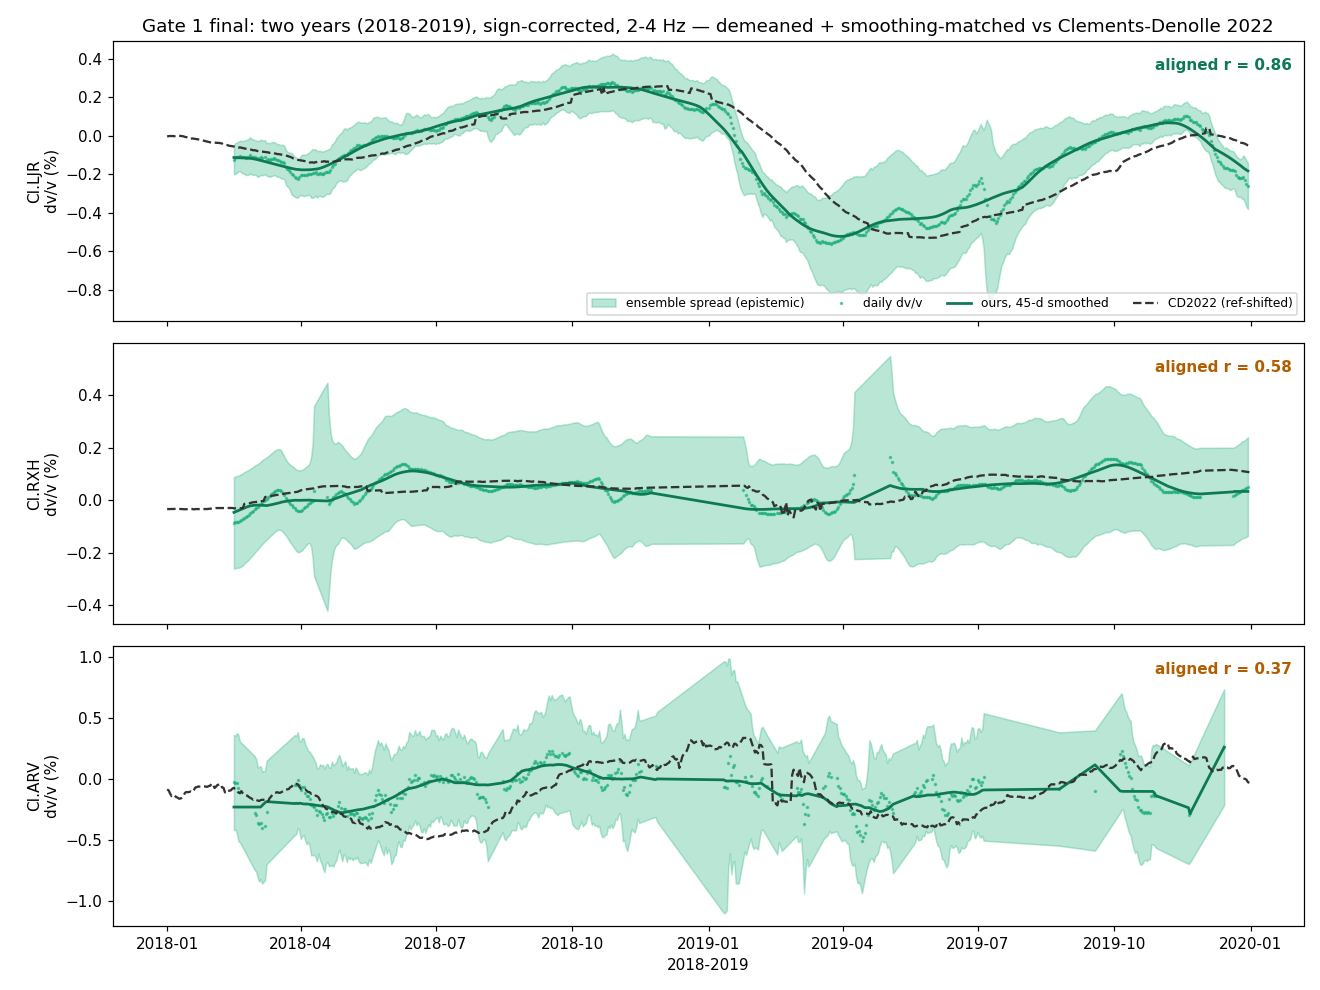
\includegraphics[width=\textwidth]{realdata_1_validation.png}
  \caption{Single-station \dvv\ at three CI stations (LJR, ARV, RXH from
  top to bottom), 2--4\,Hz, 2018--2019, against the published
  \citet{Clements2023} product (dashed; the legend names it by its 2022 data
  release). Points: the daily ensemble \dvv\ of the Gate 1 run; shading: its
  $\pm1.96\,\sigma$ band from the archived \texttt{dvv\_err} column after the
  Weaver-floor correction of \texttt{scripts/correct\_gate1\_within\_error.py}
  (Table~\ref{tab:estimands}); solid: the trailing 90-day mean of the daily
  series after the 150-day burn-in (dotted line), the matched rule of
  Table~\ref{tab:gate1}, whose Pearson $r$ and overlap are printed on each
  panel. Both smoothed series are demeaned over their overlap. Generated by
  \texttt{codameter.gate1} from the archived products and
  \texttt{paper/data/gate1/comparison.json}; the plotted arrays are in the
  figure's sidecar.}
  \label{fig:realdata-validation}
\end{figure}

Part of why agreement differs by station is visible in the correlation
function itself (Fig.~\ref{fig:realdata-interferograms}), although an
interferogram alone cannot separate a site change from an instrument or
processing change, which station metadata and processing logs would be
needed to rule out. CI.LJR shows a stable, narrow coda near zero lag
through the year. CI.RXH shows multipath, several coherent arrivals
spread across the full \(\pm 8\,\)s of lag shown, and a visible shift in
that pattern in April--May 2019, consistent with a site change rather
than a processing artefact. CI.ARV's coherent energy is compact and
concentrated near zero lag but comparatively sparse, consistent with its
higher scatter and join-method sensitivity.

\begin{figure}
  \centering
  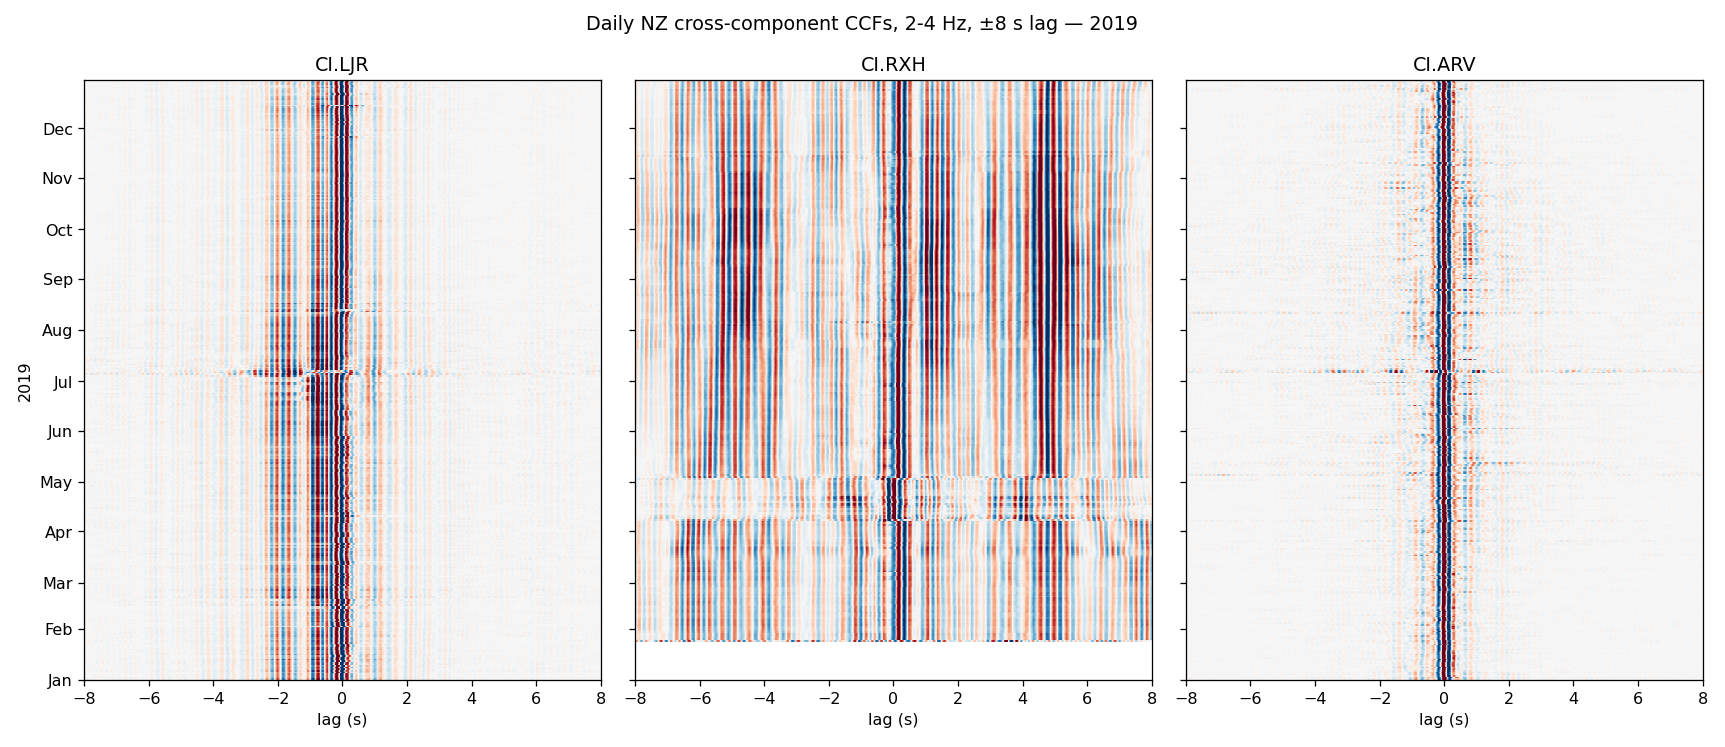
\includegraphics[width=\textwidth]{realdata_2_interferograms.png}
  \caption{Daily NZ (north-vertical) cross-component correlation functions,
  2--4$\,$Hz, $\pm 8\,$s lag, 2019, each day normalised to its maximum
  absolute amplitude (colour scale unlabelled on this externally produced
  figure). The text describes the coda character of each station and its
  relation to the station-to-station agreement of
  Fig.~\ref{fig:realdata-validation}.}
  \label{fig:realdata-interferograms}
\end{figure}

As an optional supplement, Fig.~\ref{fig:realdata-warmup} shows the
ensemble's warm-up behaviour on a separate 90-day smoke run at CI.LJR:
\dvv\(\,\)is undefined until enough history has accumulated for the
moving-reference member to compute a trailing reference, and each band's
per-epoch stretching correlation coefficient is reported alongside the
recovered series.

\begin{figure}
  \centering
  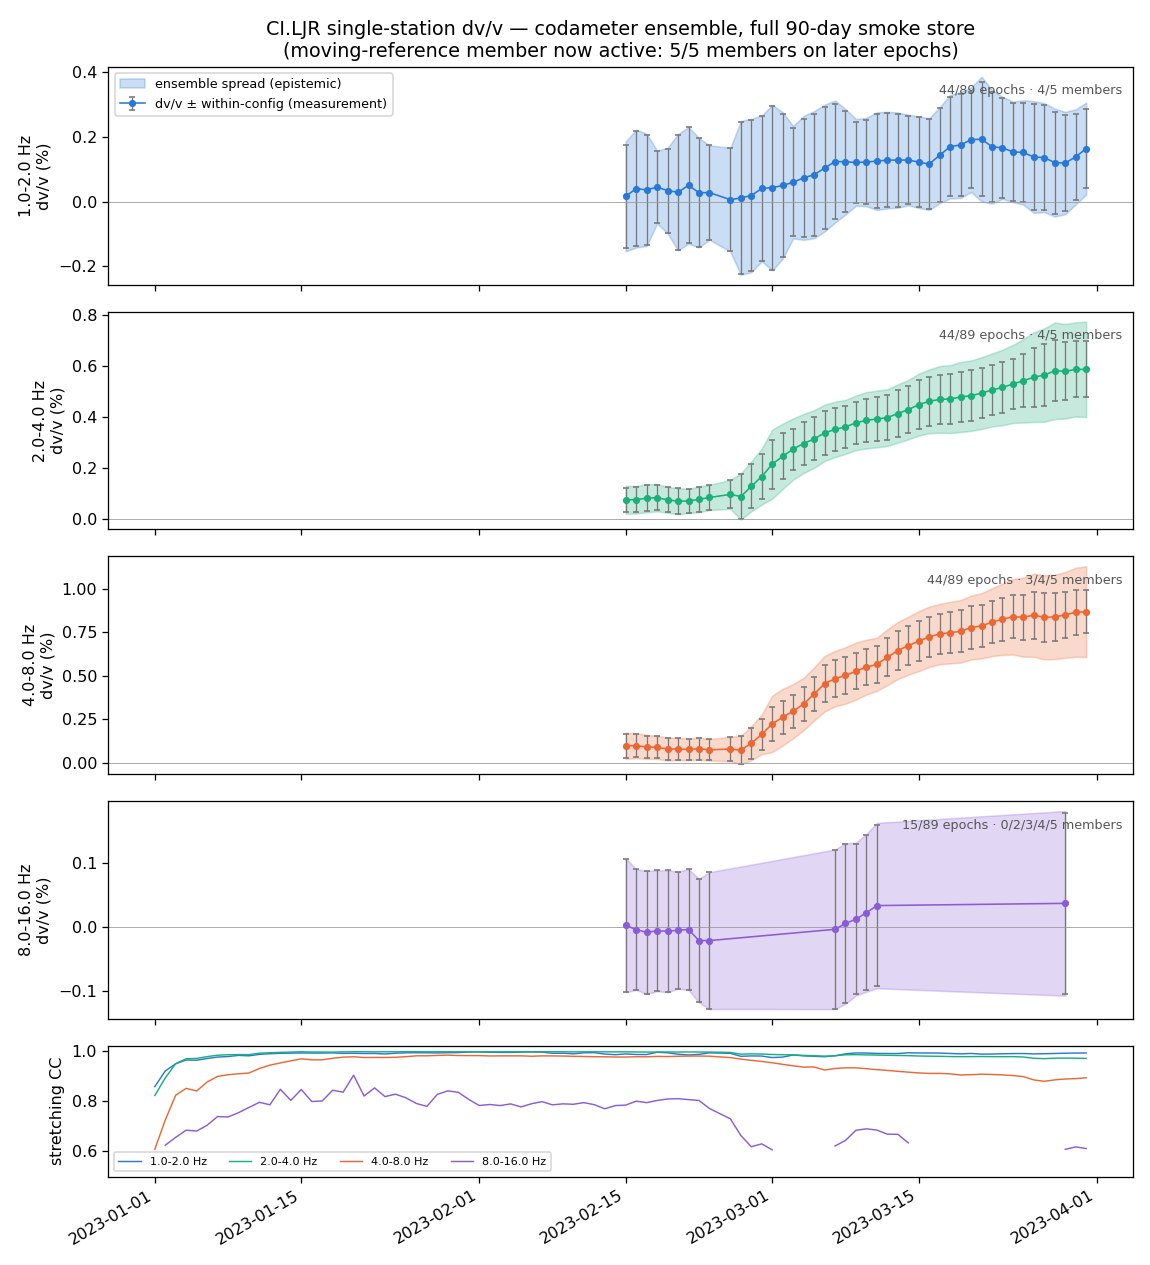
\includegraphics[width=\textwidth]{realdata_3_warmup.png}
  \caption{CI.LJR single-station \dvv, a separate 90-day smoke run (January--April
  2023), four frequency bands. The ensemble spread (shaded) and measurement
  error bars are reported once at least one member is defined. The
  annotation on each panel gives the number of epochs, out of 89, with a
  defined ensemble, followed by the set of distinct member counts, out of
  five, that occur over those epochs; counts below five arise where a member
  is undefined, for example before the moving-reference member's warm-up has
  elapsed. The figure title, written by the cloud run, names the configured
  member set; the annotations are the counts realised. Bottom panel:
  per-band stretching correlation coefficient. Produced by the cloud run,
  not regenerated here.}
  \label{fig:realdata-warmup}
\end{figure}

\section{Discussion}\label{sec:discussion}

The experiments above share one finding: on these synthetics, with one
waveform realisation held fixed, the processing choice moves both the
recovered \dvv~and its stated uncertainty by more than the measurement
noise does, by two orders of magnitude in RMS across the 108-pipeline
multiverse and by a factor \(\sqrt{N}\) in the reported network error
bar. Whether processing also dominates the variability between real
deployments is a question these experiments cannot answer, because they
hold the observed waveform fixed; the repeated-realisation calibration
of Section~\ref{sec:bayes} is the first step toward it. The problem is
consequential but tractable. We suggest the following responses.

\textbf{Report the choices.} At minimum, a \dvv~study should state the
estimator and its parameters, the frequency band(s) and coda window(s)
and how the window was set relative to the band, the reference scheme,
the stacking, the cross-component and station-pair aggregation \emph{and
weighting}, and --- critically --- the exact definition of the quoted
uncertainty (within-measurement error, between-component/pair standard
error, or standard deviation). Our results show that the last item alone
changes the number quoted as \(1\sigma\) by \(\sqrt{N}\), because the
two conventions estimate different quantities
(Table~\ref{tab:estimands}). Table~\ref{tab:checklist} collects this
into a minimal reporting checklist, and Appendix~\ref{app:survey} shows
how unevenly these items are reported across the literature today.

\begin{table}
\footnotesize
\caption{A minimal reporting checklist for an ambient-noise \dvv\ study. Stating
these turns an undocumented, irreproducible choice into an inspectable one and
makes error bars comparable across studies.}
\label{tab:checklist}
\begin{tabularx}{\textwidth}{@{}>{\raggedright\arraybackslash}p{3.4cm} L@{}}
\toprule
\textbf{Step} & \textbf{What to report} \\
\midrule
Pre-processing & Time-domain normalization (one-bit / running-mean), spectral
whitening band, sampling rate \\ \hline
Correlation \& stacking & Components computed, segment length, daily/sub-stack
length, total reference span \\ \hline
Estimator & Method (TS / WCC / DTW / MWCS / WCS / WTS / WTDTW), its parameters
($\varepsilon$-grid, or sub-window length and step), and whether the phase is
unwrapped \\ \hline
Frequency band(s) & $[f_1,f_2]$ for every reported measurement \\ \hline
Coda window(s) & $[t_1,t_2]$, the branch(es) used, and \emph{how} $t_1,t_2$ were
set relative to the band \\ \hline
Reference & Scheme (total stack / trailing / inversion) and period \\ \hline
Component aggregation & Approach A or B; weighted (by what) or unweighted \\ \hline
Pair / network aggregation & Spatial averaging and weighting scheme \\ \hline
Uncertainty & The exact definition of the quoted error: within-measurement
(e.g.\ Weaver), between-component/pair standard error, or standard deviation \\ \hline
Quality control & CC / SNR thresholds, rejection criteria, resulting effective
$N$ \\ \hline
Software & Package, version, and the parameter file or its DOI \\
\bottomrule
\end{tabularx}
\end{table}

\textbf{Quantify the choice-induced uncertainty.} Where a choice is not
forced by the physics, it can be sampled. Pushing a distribution of
reasonable processing choices through the same correlations measures
conditional sensitivity. A probabilistic mixture would combine
conditional variances and the variance of conditional means. The joint
likelihood in Section~\ref{sec:bayes} instead defines a working Bayesian
model whose deliverable is a time-dependent single-measurement
covariance \(C_d\). Its limitations are as important as its
construction. The prior over pipelines is a menu, not a representative
sample of practice, and the covariance is conditional on it. Every
configuration transforms the same waveforms, so an error they all share
(a source change, a contaminated reference, a clock drift measured on
one branch) leaves no trace in their spread: on the shared-source
scenario of Table~\ref{tab:calibration} the ensemble agrees with itself,
the error of its mean doubles, and \(C_d\) cannot see it. Configurations
in different bands sample different depths and may not estimate the same
physical quantity, so the configuration axis should be marginalised only
over pipelines that target one estimand. And the coherence floor of
\citet{Weaver2011} is a lower bound: on our synthetic the residual
scatter about the ensemble mean is an order of magnitude above it, which
the fitted rescale \(s\) reports rather than hides. The pointwise tests
in Table~\ref{tab:calibration} support the \(95\,\%\) member intervals
on the listed scenarios. They also expose \(68\,\%\) overcoverage and
poor coverage of the combined estimate. They do not establish temporal
covariance calibration, convergence across independent chains, or valid
downstream intervals.

\textbf{Make it executable.} All synthetics, estimators and generated
figures in this paper are released in the open codameter package; one
driver regenerates every generated figure together with a numerical
sidecar holding every plotted array and the run's provenance, and the
package is unit-tested. Of the three real-data figures, the comparison
(Fig.~\ref{fig:realdata-validation}) is regenerated by the same driver
from the archived daily products; the interferograms and the warm-up
figure were produced by the cloud run from correlations that are not
archived here and are committed as produced
(Section~\ref{sec:deployment}). An executable record turns an
undocumented choice into a versioned, inspectable one, and lets a reader
re-run a study's pipeline on the truth-known synthetic to see its bias
before trusting it on data.

\textbf{Validate against something you did not generate.} Every
synthetic test in this paper passed before the discovery below, and that
is exactly the danger: a synthetic built under the same sign convention
as the estimator reading it will always agree, whether the convention is
physically correct or not. Testing codameter's estimators against a real
cross-network deployment (Section~\ref{sec:deployment}), recovered
\dvv~anticorrelated with the published \citet{Clements2023} product and
with seasonal hydrology at all three stations under the rule used at the
time. The coefficients of that first run were not archived; the
qualitative record is the codameter v0.4.0 release note, and the
corrected comparison is Table~\ref{tab:gate1}. Ground-truthing through
the exact call path made the cause obvious: imposing a \(+0.5\,\%\)
velocity change returned \(-0.50\,\%\). The synthetic generator and all
seven estimators had consistently used the stretch factor
\(\varepsilon\) (positive for a coda dilation, i.e.~a slowdown), not
physical \dvv~(positive for a speedup) --- internally coherent, so every
synthetic-recovery test in the sections above passed, but opposite to
the sign convention the field expects and to the published product it
was compared against. The fix is the convention boxed in
Section~\ref{sec:intro}, shipped as codameter v0.4.0. Internal
consistency is not correctness: a pipeline that only checks itself will
confirm whatever convention it started with, and only the comparison
against an independently-produced result caught this one. The fix and
its ground-truthing procedure are documented in the codameter release
history.

\textbf{Propagate the covariance, do not truncate it.} The measurement
covariance is not the end of the analysis but its first input.
Section~\ref{sec:depth} sets out the next step of the chain: invert the
per-band \(C_d\) through sensitivity kernels for a depth profile and its
covariance, separating the shear-velocity and density contributions
where the ground is partially saturated. Converting that depth-resolved
posterior to stress or strain requires material priors this paper does
not attempt to constrain, and is left to other work. What codameter
provides today is the interface that consumes \(C_d\); the depth
posterior itself, its resolution, and the calibration of its covariance
are not demonstrated in this paper. Building and testing the
depth-propagation stage on truth-known synthetics with overlapping
kernels is the natural continuation of this work.

\section{Conclusions}\label{sec:conclusions}

Ambient-noise \dvv~monitoring rests on a chain of processing choices
that are made ad hoc and reported incompletely. Using a truth-known
synthetic and the full estimator suite of an open toolbox, we have shown
that these choices change the RMS error of the recovered \dvv~by more
than two orders of magnitude (0.02 to \(2.8\,\%\)) across 108 pipelines
on one synthetic volcano scenario and, more consequentially, change the
number reported as its uncertainty by a factor of \(\sim\!\sqrt{N}\)
depending on whether a study calls \(1\sigma\) the standard error of the
network mean or the between-pair standard deviation, all without
touching the data. The remedy is not a single mandated pipeline but
transparency: report every choice and name the quantity each error bar
estimates, sample the choices the physics does not fix, carry the
resulting measurement covariance into the inference after validating
what it is meant to cover, and release the pipeline as executable code.
Repeated synthetic realisations support the proposed \(95\,\%\)
pointwise intervals for the error of a single processing configuration,
while the nominal \(68\,\%\) intervals overcover and the credible band
on the ensemble mean undercovers (Table~\ref{tab:calibration}). The
temporal correlation in \(C_d\) is untested, a cross-band covariance is
not constructed, and an error shared by every configuration is
demonstrably invisible to the ensemble. A depth inversion also needs
kernel uncertainty and the covariance of the actual observations it
consumes. Converting a depth profile to stress or strain is a further
step this paper does not attempt. We offer codameter as one such record;
its depth stage is an interface awaiting evaluation.

\appendix

\section{Estimator definitions}\label{app:estimators}

Let \(r(t)\) and \(c(t)\) be the reference and current
cross-correlations, band-passed to \([f_1,f_2]\) (central frequency
\(f_c\), bandwidth \(B\)) and read over the coda window \(W=[t_1,t_2]\)
on one or both branches. Each method below estimates either the stretch
factor \(\varepsilon\), the fractional dilation of the current coda
relative to the reference, which is then mapped to physical \dvv~through
the convention boxed in Section~\ref{sec:intro},
\(\dvv=-\varepsilon/(1+\varepsilon)\), or a slope of delay against lapse
that is reported as \dvv~directly; the convention paragraph before the
delay-based methods says which route each estimator takes.

\textbf{Trace stretching (TS).} For each trial stretch factor
\(\varepsilon\), the current correlation is interpolated as
\(c_\varepsilon(t)=\mathcal{I}[c]\big((1+\varepsilon)t\big)\)
(interpolation on current only) while the reference \(r(t)\) remains
fixed. The windowed correlation coefficient is \begin{equation}
\mathrm{CC}(\varepsilon) = \frac{\int_W r(t)\,c_\varepsilon(t)\,\mathrm{d}t}
{\left(\int_W r^2\,\mathrm{d}t\int_W c_\varepsilon^2\,\mathrm{d}t\right)^{1/2}},
\qquad \varepsilon^\star = \arg\max_\varepsilon \mathrm{CC}(\varepsilon).
\end{equation} The best-fit stretch \(\varepsilon^\star\) is then
converted to physical \(\dvv\) via
\(\dvv^\star = -\varepsilon^\star/(1+\varepsilon^\star)\) as boxed in
the Introduction. The single-measurement error decreases with the
coherence \(\mathrm{CC}\), the bandwidth \(B\), and the window length.
We use eq.~20 of \citet{Weaver2011}, \begin{equation}
\sigma_{\varepsilon} = \frac{\sqrt{1-\mathrm{CC}^2}}{2\,\mathrm{CC}}
\sqrt{\frac{6\sqrt{\pi/2}\;T}{\omega_c^2\,(t_2^3-t_1^3)}},
\qquad T=\frac{\sqrt{\ln 10}}{\pi B},
\label{eq:weaver}
\end{equation} with \(\omega_c=2\pi f_c\) and \(T\) the spectral
timescale of Weaver et al.'s Gaussian spectrum, fixed here by placing
the band edges at that spectrum's \(-10\),dB points; any convention with
\(T\propto 1/B\) gives the same \(1/\sqrt{B}\) scaling and differs by a
constant that the rescale \(s\) of Section~\ref{sec:bayes} absorbs. The
corresponding error on \dvv~follows from the exact map,
\(\sigma_{\dvv}=\sigma_{\varepsilon}/(1+\varepsilon)^2\), which equals
\(\sigma_{\varepsilon}\) to first order. (The codameter implementation
before this revision omitted \(T\) and used a variance prefactor twice
this one; the fitted \(s\) absorbed the constant, and only the relative
weighting of configurations in different bands changed when it was
corrected.)

\emph{Interpolation direction and convention.} The interpolation is
applied to the current waveform and not the reference so that the
high-SNR reference stack remains invariant throughout the epsilon
search, which is particularly important when the reference is built as a
long-term or moving average. In the continuous-signal, infinite-support
limit the two conventions (interpolating current versus interpolating
reference) are mathematically equivalent after their fitted parameters
are converted to the same physical \(\dvv\) through the exact relation
\(\dvv = -\varepsilon/(1+\varepsilon)\). In sampled, finite-window
signals, that symmetry is broken: interpolation error, edge truncation,
and the finite support of the data cause the two conventions to give
slightly different numerical results even when both use the exact
conversion. Therefore the interpolation direction must be reported
explicitly and treated as a fixed processing choice. For diffuse codas
in ambient-noise and volcanic monitoring, we have verified that the
choice has a measurable but small effect: truth-known synthetics recover
\(\dvv\) with sub-\(10^{-4}\) bias when the signal-to-noise ratio is
high and the changes are small, with the effect growing as a few percent
at landslide-scale perturbations (\(\dvv\sim4\,\%\)).

Throughout this appendix a delay \(\delta t\) is the lag of the current
trace relative to the reference, positive when the current arrival is
later, so for the pure dilation \(c(t)=r(t/(1+\varepsilon))\) a phase at
reference lapse \(t_i\) appears at \((1+\varepsilon)t_i\) and
\(\delta t_i=+\varepsilon\,t_i\). The implementation uses the Fourier
convention
\(\hat c(f)=\int c(t)\,e^{-2\pi\mathrm{i} f t}\,\mathrm{d}t\), under
which a delay by \(\delta t\) multiplies \(\hat c\) by
\(e^{-2\pi\mathrm{i} f\,\delta t}\). The estimators reach \dvv~by two
routes. TS, WCC and WTS fit the dilation \(\varepsilon\) and apply the
exact map \(\dvv=-\varepsilon/(1+\varepsilon)\). MWCS, WCS, DTW and
WTDTW fit a slope of delay or lag against lapse and report that slope as
\dvv~without a further map: for the two phase methods the fitted slope
is \(-\varepsilon\), which equals \dvv~to first order in
\(\varepsilon\); for the two warping methods the lag path runs from the
current to the reference sample, so the slope of the ideal path is
\(1/(1+\varepsilon)-1=-\varepsilon/(1+\varepsilon)\), which is
\dvv~exactly. A regression test in codameter imposes \(\dvv=+0.3\,\%\)
and \(-0.4\,\%\) on a noise-free coda and holds every estimator to the
imposed value within \(10^{-3}\); at these amplitudes the first-order
slope and the exact map differ by
\(\varepsilon^2/(1+\varepsilon)\approx10^{-5}\), so the test fixes the
sign but does not separate the two routes.

\textbf{Windowed cross-correlation (WCC).} In sub-windows (6 s long, 3 s
step) centred at lapse \(t_i\) the delay is
\(\delta t_i=\arg\max_{\tau}\int c(t)\,r(t-\tau)\,\mathrm{d}t\); a
least-squares fit of \(\delta t_i=\varepsilon\,t_i\) gives
\(\varepsilon\).

\textbf{Moving-window cross-spectrum (MWCS).} In each sub-window (6 s
long, 3 s step) the cross-spectrum is \(X(f)=\hat c(f)\,\hat r^{*}(f)\)
with phase \(\varphi(f)=\arg X(f)=-2\pi f\,\delta t_i\) under the stated
convention. \citet{Clarke2011} fit \(\varphi(f)\) linearly over
\([f_1,f_2]\) with coherence weights; the implementation used here reads
one phase from the band-summed cross-spectrum at the power-weighted
centre frequency \(f_c\) of the sub-window,
\(\varphi/(2\pi f_c)=-\delta t_i\), and the slope of that quantity
against \(t_i\), which is \(-\varepsilon\), is reported as \dvv. Because
\(\varphi\) is defined modulo \(2\pi\), the estimate cycle-skips once
\(|\delta t_i|>1/(2f_c)\).

\textbf{Dynamic time warping (DTW).} A lag path \(l(i)\) minimises
\begin{equation}
\sum_i \big(c_i - r_{i+l(i)}\big)^2 \;+\; \gamma\sum_i \big(l(i{+}1)-l(i)\big)^2,
\end{equation} where \(\gamma=0.3\) penalises strain (limits the lag's
rate of change) and the lag is bounded by \(0.8\) s. The path maps
current sample \(i\) to reference sample \(i+l(i)\), so for a pure
dilation \(l(i)/f_s=t_i\,[1/(1+\varepsilon)-1]\) and the slope of
\(l(i)/f_s\) against lapse is \(-\varepsilon/(1+\varepsilon)\), reported
directly as \dvv.

\textbf{Wavelet cross-spectrum (WCS).} With continuous wavelet
transforms \(W_c,W_r\), the cross-wavelet spectrum is
\(W_{xy}(f,\tau)=W_c\,W_r^{*}\) with phase
\(\varphi(f,\tau)=-2\pi f\,\delta t(f,\tau)\) under the stated
convention. Unwrapping \(\varphi\) in two dimensions, along lapse
(anchored at \(\tau\!\to\!0\), where \(\delta t\!\to\!0\)) then along
frequency, removes the cycle-skip; the \(|W_{xy}|\)-weighted regression
of \(\varphi/(2\pi f)\) on \(\tau\) over the time--frequency window
gives the slope \(-\varepsilon\), which is reported as
\dvv~\citep{Mao2020}.

\textbf{Wavelet stretching / warping (WTS, WTDTW).} WTS applies the
stretch search of TS to the real part of each wavelet-scale row of the
current transform against the fixed reference row, pools the per-scale
\(\varepsilon\) with weights equal to the norm of the current row in the
window, and applies the exact map to the pooled \(\varepsilon\). WTDTW
sums the real part of the transform over the band into one
wavelet-filtered trace and applies the DTW of the previous paragraph to
it, reporting the lag slope as \dvv.

\section{Aggregation and uncertainty conventions}\label{app:aggregation}

For component \(k\) of a station pair, stretching yields the image
\(\mathrm{CC}_k(\varepsilon,t)\); each per-component stretch factor
converts to physical \(\dvv_k\) via the boxed relation.

\textbf{Approach A (average the per-component \dvv).} \(\dvv_k(t)\)
follows from \(\varepsilon_k(t)=\arg\max_{\varepsilon}
\mathrm{CC}_k(\varepsilon,t)\), and the pair estimate is the (possibly
weighted) mean \(x_p(t)=\sum_k w_k\,\dvv_k/\sum_k w_k\), with
\(w_k=\max_{\varepsilon}
\mathrm{CC}_k\) (coherence-weighted) or \(w_k=1\) (unweighted).

\textbf{Approach B (average the images).} The pair stretch factor
\(\varepsilon_p(t)=\arg\max_{\varepsilon}\big[\tfrac1{N_c}\sum_k
\mathrm{CC}_k(\varepsilon,t)\big]\) converts to \(x_p(t)=\dvv_p(t)\) via
the same relation.

\textbf{Network over pairs.} With pair weights \(W_p\) (e.g.~mean
coherence), \begin{equation}
\bar x=\frac{\sum_p W_p x_p}{\sum_p W_p},\quad
s^2=\frac{\sum_p W_p (x_p-\bar x)^2}{\sum_p W_p},\quad
N_{\mathrm{eff}}=\frac{(\sum_p W_p)^2}{\sum_p W_p^2}.
\end{equation} The three uncertainty conventions used in
Section~\ref{sec:uncertainty} are the weighted standard error
\(\sigma_{\mathrm{SE},w}=s/\sqrt{N_{\mathrm{eff}}}\), the unweighted
standard error \(\sigma_{\mathrm{SE}}=\mathrm{std}(x_p)/\sqrt{N}\), and
the standard deviation \(\sigma_{\mathrm{SD}}=\mathrm{std}(x_p)\). They
share the mean \(\bar x\) but obey
\(\sigma_{\mathrm{SD}}/\sigma_{\mathrm{SE}}=\sqrt{N}\).

\section{Survey of processing choices across the
literature}\label{app:survey}

Table~\ref{tab:survey} catalogues the processing choices of the
ambient-noise \dvv~monitoring studies we surveyed: 103 rows for 103
publications, one per publication (the full machine-readable version and
provenance are distributed with the codameter package). It is the
empirical basis for the paper's claim that no convention is shared: the
estimator, the frequency band, the coda window, the reference scheme and
--- most unevenly of all --- the uncertainty treatment vary study to
study, and the last is frequently unreported. Every study is cited here.

The four measurement fields (frequency band, coda window, estimator and
uncertainty treatment) were re-checked against the \emph{full text} for
the 82 studies we could read (open access plus institutional access);
for those rows a blank or
\texttt{n/r\textquotesingle{}\textquotesingle{}\ means\ the\ value\ is\ genuinely\ not\ stated\ in\ the\ paper.\ The\ remaining\ rows\ were\ populated\ from\ abstracts\ and\ search\ metadata,\ where}n/r'\,'
means only that the value was not found in the abstract, not that the
study failed to report it; those cells are flagged in the
machine-readable table (\texttt{measurement\_source}) and remain to be
filled from the paywalled full texts. Because a cell populated from an
abstract can only move from ``n/r'\,' to reported once the full text is
read, the apparent under-reporting in the table is an upper bound on the
true under-reporting; the verified rate is the one among the 82
full-text rows.

% Auto-generated by paper/build_survey.py -- do not edit by hand.
{\footnotesize
\setlength{\tabcolsep}{3pt}
\renewcommand{\arraystretch}{1.15}
\begin{longtable}{@{}p{2.1cm} >{\raggedright\arraybackslash}p{1.9cm} >{\raggedright\arraybackslash}p{1.5cm} >{\raggedright\arraybackslash}p{1.3cm} >{\raggedright\arraybackslash}p{1.5cm} >{\raggedright\arraybackslash}p{2.4cm} >{\raggedright\arraybackslash}p{3.0cm}@{}}
\caption{Processing choices of the 103 surveyed \dvv\ studies (the literature survey underpinning this paper). Every study is cited; \texttt{n/r} = not reported in the source. Frequency band, coda window, estimator, reference/stack scheme and uncertainty treatment are the choices Section~\ref{sec:results} shows to control the result.}\label{tab:survey}\\
\toprule
\textbf{Study} & \textbf{Site / region} & \textbf{Freq (Hz)} & \textbf{Coda (s)} & \textbf{Method} & \textbf{Reference / stack} & \textbf{Uncertainty treatment} \\
\midrule
\endfirsthead
\multicolumn{7}{@{}l}{\footnotesize\itshape Table~\ref{tab:survey} continued}\\
\toprule
\textbf{Study} & \textbf{Site / region} & \textbf{Freq (Hz)} & \textbf{Coda (s)} & \textbf{Method} & \textbf{Reference / stack} & \textbf{Uncertainty treatment} \\
\midrule
\endhead
\midrule\multicolumn{7}{r@{}}{\footnotesize\itshape continued on next page}\\
\endfoot
\bottomrule
\endlastfoot
\citet{Brenguier2008} & Piton de la Fournaise, La Réunion & 0.5–2 & n/r & Stretching & Daily stacks referenced to long-term stack & Compared against \textasciitilde{}0.05\% measurement precision / noise floor \\
\citet{Duputel2009} & Piton de la Fournaise, La Réunion & 0.1–1 & n/r & Other & Quasi-real-time stacks vs reference & n/r \\
\citet{Obermann2013} & Piton de la Fournaise, La Réunion & >0.5 & increasing lapse-time coda windows & Stretching & Daily stacks, referenced; coda at increasing lapse times & n/r \\
\citet{HotovecEllis2014} & Mount St. Helens, WA, USA & >5 (high-frequency repeating earthquakes) & n/r & Other & Stack across several hundred repeating-earthquake families (multiplets) & n/r \\
\citet{HotovecEllis2015} & Mount St. Helens, WA, USA & n/r & n/r & Other & Combines repeating-earthquake CWI with ambient-noise interferometry & n/r \\
\citet{Rivet2015} & Piton de la Fournaise, La Réunion & n/r & n/r & Stretching & Daily stacks vs reference; network-averaged dv/v & dv/v corrected for rainfall pore-pressure to improve detectability of small drops \\
\citet{DePlaen2016} & Piton de la Fournaise, La Réunion (method also re Kawah Ijen) & 0.1–1.0 (drop visible); best SNR 0.5–1 and 1–2 & n/r & Stretching & n/r & n/r \\
\citet{Donaldson2017} & Kīlauea summit, Hawaii, USA & 0.33–1.0 (lava-lake tremor band) & up to \textasciitilde{}120 (min lag set by inter-station distance to tremor source) & MWCS & Daily NCFs stacked over 3-day moving window & Reject pairs when MWCS regression error too large; accept if coherence high (>\textasciitilde{}0.65) \\
\citet{Takano2017} & Izu-Oshima, Japan & 0.5–1; 1–2; 2–4 (depth discrimination) & n/r & n/r & Cross-correlations 2012–2015, multiple bands & n/r \\
\citet{Lesage2018} & Volcán de Colima, Mexico & 0.125–2 & n/r & Stretching & Daily cross-correlations; 2013 stack as reference & Pair averaging → <0.05\% noise floor; clock-sync errors identified and corrected \\
\citet{DePlaen2019} & Mt. Etna, Italy (2013–2014) & 1–2 & 5–35 (causal + acausal lags) & MWCS & Daily autocorrelations, 2-day linear stack & Median errors \textasciitilde{}0.03\%/station; reject if dt error >0.1 s and coherence <0.6 \\
\citet{Donaldson2019} & Northern Volcanic Zone (Askja/Bárðarbunga), Iceland & multiple bands for depth discrimination (n/r exact) & n/r & n/r & n/r & n/r \\
\citet{Olivier2019} & Kīlauea, Hawaii, USA (2018 eruption) & 0.1–0.2 (secondary microseism); 0.3–1 (volcanic tremor) & n/r & Stretching & n/r (passive image interferometry, daily) & Resolves <0.1\%; cross-checked vs GPS/tilt \\
\citet{Yates2019} & Whakaari / White Island, New Zealand & n/r & n/r & n/r & n/r & n/r \\
\citet{Feng2020} & Kīlauea, Hawaii, USA & 0.3–0.6; 0.6–0.9; 0.9–2.0 & n/r & n/r & Jan 2017–Jun 2018 NCFs & n/r \\
\citet{HotovecEllis2022} & Kīlauea, Hawaii, USA (2018 collapse) & n/r & n/r & Other & Coda Wave Interferometry with Repeating Earthquakes (CWIRE), per-cluster pairs & n/r \\
\citet{Kopfli2024} & Mount St. Helens, WA, USA & n/r & n/r & Other & Long-term NCF stacks; many dv/v series on a common grid & n/r \\
\citet{Yates2024} & Mt. Ruapehu, New Zealand (2005–2009) & n/r & n/r & Wavelet & n/r & n/r \\
\citet{Yukutake2025} & Izu-Oshima, Japan (2003–2020) & 0.5–2.0 & n/r & n/r & Long-term interferometry stacks, 2003–2020 & n/r \\
\citet{Schaff2004} & 1989 Mw 6.9 Loma Prieta aftershock zone, California (also Parkfield repeaters) & n/r & n/r & Other & Repeating-earthquake doublets; delays vs pre-mainshock repeaters & High-precision relative delay via waveform cross-correlation of near-identical repeaters \\
\citet{Pacheco2005} & Theory / acoustic diffusion model & n/r & n/r & Other & n/r & n/r (analytical kernel) \\
\citet{Rubinstein2005} & 2004 M6 Parkfield earthquake, San Andreas fault, California & n/r & n/r & Other & Repeating-earthquake travel-time delays before vs after mainshock & Precise relative delay from near-identical repeating-earthquake waveforms \\
\citet{Wegler2007} & Mid-Niigata (Chuetsu) earthquake source region, Japan; F-Net station KZK (\textasciitilde{}24 km) & 2–50 (2 Hz high-pass; 100 Hz data) & 5–14 & Stretching & Daily autocorrelations vs \textasciitilde{}two-week pre-event reference; grid search (10000 trials, dv/v… & ±0.1\% fluctuation = inversion accuracy \\
\citet{Brenguier2008b} & Parkfield, San Andreas fault, California, USA & 0.1–0.9 & n/r & Stretching & 1550-day reference vs overlapping 5-day moving windows; 30-day time resolution & Averaged over 78 receiver pairs plus 5-day segments \\
\citet{Hadziioannou2009} & Laboratory scattering gel (ultrasonic) & 2.5e6 (2.5 MHz lab) & n/r & Other & Noise-correlation stacking & Demonstrates stability when background noise-source structure is stable \\
\citet{Sawazaki2009} & Western-Tottori region, Japan; KiK-net borehole (surface + 100 m); 2000 Mw 6.6 mainshock & n/r & n/r & Other & Coda deconvolution of surface vs 100-m borehole records & n/r \\
\citet{Wegler2009} & 2004 Mw 6.6 Mid-Niigata earthquake source region, Japan; 6 Hi-net/F-Net stations <25 km & n/r & n/r & Stretching & Daily auto-/cross-correlations inverted daily for 2 months pre/post; pre-event reference & Daily inversion fluctuations; consistency across 6 stations \\
\citet{Chen2010} & Sichuan, China — 2008 Mw 7.9 Wenchuan earthquake fault zone & n/r & n/r & Other & Noise cross-correlation stacking; sub-array comparison (156 broadband stations) & Pre-earthquake fluctuation (\textasciitilde{}0.02\%) used as baseline/noise reference \\
\citet{Nakata2011} & NE Japan (Honshu), KiK-net; 2011 Tohoku-Oki earthquake & n/r & n/r & Other & >300 earthquakes (Jan 1–May 26 2011); borehole-to-surface deconvolution & n/r \\
\citet{Rivet2011} & Guerrero, Mexico subduction zone (2006 M7.5 slow slip event) & 0.06–0.14 (periods 7–17 s) & n/r & MWCS & n/r & n/r \\
\citet{Hobiger2012} & 2008 Iwate-Miyagi Nairiku earthquake (Mw 6.9), NE Japan & 0.125–1.0 (three sub-bands) & n/r & Stretching & Daily cross-correlations vs long-term reference Green's function & Curves fit by model (coseismic drop + log postseismic recovery + seasonal) \\
\citet{Minato2012} & Southern Tohoku (Fukushima/Ibaraki), Japan; 58 Hi-net stations; 2011 Tohoku-Oki & n/r & n/r & Stretching & n/r & n/r \\
\citet{Obermann2013} & Numerical 2-D elastic media (lunar-data illustration) & central 20 (bandwidth \textasciitilde{}12) & 1.8–6.6 (primary lapse \textasciitilde{}3.6 s) & Stretching & Averaged over 10 random medium realizations per configuration & S.d. over 10 realizations; mean-free-path uncertainty \textasciitilde{}2–15\% \\
\citet{Brenguier2014} & Volcanic/geothermal regions of Honshu, Japan; 2011 Mw 9.0 Tohoku-Oki & 0.1–0.9 & n/r & MWCS & Daily cross-correlations; linear inversion/regularization for continuous time series & Stress sensitivity \textasciitilde{}0.001 MPa\textasciicircum{}-1 inferred; detailed dv/v uncertainty n/r \\
\citet{Liu2014} & Epicentral region of 2008 Mw 7.9 Wenchuan earthquake, China & 0.25–0.5 (period 2–4 s most sensitive) & n/r & Stretching & Noise cross-correlation stacking (Aug 2004 – Sep 2011) & Pre-event period as baseline (no obvious precursor) \\
\citet{Taira2015} & South Napa, California (2014 Mw 6.0 South Napa earthquake) & 0.08–2.0 & n/r & MWCS & MSNoise cross-correlations; decimated to 20 Hz & n/r \\
\citet{Gassenmeier2016} & Station PATCX, Atacama Desert, Northern Chile (IPOC) & 4–6 primary (also 1–3, 7–10) & 10–15 primary (also 5–10, 15–20) & Stretching & Daily autocorrelations; two-step iterative reference & Error from correlation-coefficient threshold ±1 s.d.; healing-fit errors (amplitude \textasciitilde{}21\%… \\
\citet{Hillers2019} & San Jacinto fault zone, California (after 2010 M7.2 El Mayor-Cucapah, M5.4 Collins Valley) & n/r & n/r & Stretching & Average-waveform reference for stretching; MWCS also applied & Cross-check between time-domain stretching and frequency-domain MWCS \\
\citet{Wang2019} & NE Honshu, Japan (2011 Mw 9.0 Tohoku-Oki earthquake) & 0.02–1.0 (period 1–50 s; short-period 1–7 s + tiltmeters 8–50 s) & n/r & Stretching & Monthly velocity-change estimates & n/r \\
\citet{Mao2020} & Salton Sea Geothermal Field, California (2009–2011) & frequency-dependent across band (time-frequency domain) & full time-frequency domain & Wavelet & Noise cross-correlation stacking & Wavelet-coherence thresholding and amplitude-based weighting \\
\citet{Poli2020} & L'Aquila region, central Italy (2009 Mw 6.3 L'Aquila earthquake) & n/r & n/r & n/r & n/r & n/r \\
\citet{Boschelli2021} & Ridgecrest fault zone, California (2019 Mw 7.1 Ridgecrest earthquake) & n/r & n/r & Other & Daily autocorrelation functions vs mean waveform & n/r \\
\citet{Lu2021} & Ridgecrest, California (2019 Mw 7.1 Ridgecrest earthquake) & 8.0–12.0 & 3 (moving windows, 1.5 s step) & Other & 10-min stacks; adaptive Gaussian smoothing (20 min growing to 24 hr over 3 days) & Standard deviations tracked; stabilized via smoothing \\
\citet{Sheng2022} & San Jacinto fault, Anza seismic gap, Southern California & >1.0 & n/r & Wavelet & Weekly stacked correlations with \textasciitilde{}2-month smoothing & Inverse travel-time uncertainties used as weights in misfit \\
\citet{Mainsant2012} & Pont-Bourquin landslide, Swiss Alps (Switzerland) & \textasciitilde{}4-10 (band of measured surface-wave dv/v; spectral analysis up to \textasciitilde{}12) & n/r (short inter-sensor distance, coda of daily correlograms) & Stretching & Daily noise correlograms (cross-correlation functions) & Daily correlation-coefficient / waveform-coherence checks; qualitative \\
\citet{Voisin2016} & Avignonet / Mas d'Avignonet landslide, Trièves (French Alps), France & \textasciitilde{}6-8 (annual dv/v pattern best resolved) & n/r & Stretching & Daily/seasonal stacks vs reference & Correlation-coefficient weighting; comparison with piezometer \\
\citet{Harba2017} & Just-Tęgoborze landslide, Carpathian flysch, southern Poland & High-frequency seismic noise (\textasciitilde{}5-20+, dispersion-curve range) & n/r (interferometric Green's-function retrieval) & Other & Cross-correlation / interferometric stacks; dispersion inversion (neighbourhood algorithm) & Dispersion-inversion misfit; comparison with MASW \\
\citet{Bertello2018} & Montaguto earthflow, southern Italy & n/r (surface-wave / MASW band, \textasciitilde{}few-20) & n/r & Other & Time-lapse interferometry + time-lapse active MASW & Comparison passive vs active MASW; qualitative \\
\citet{Bievre2018} & Pont-Bourquin landslide, Swiss Alps (4.5-yr record) & \textasciitilde{}5-15 (surface-wave band; reported sensitivity to shallow layer <=2 m) & n/r & Stretching & Daily correlations, multi-year reference & Correlation coefficient; seasonal-cycle modeling to separate from precursors \\
\citet{Colombero2018} & Madonna del Sasso cliff, NW Italian Alps (Orta Lake), Italy & 2-20 (analysis); 2-4 strongest annual signal & 0.5-2 (and symmetric -2 to -0.5) & Stretching & Daily correlations, multi-year reference (2013-2016) & Correlation coefficient (\textasciitilde{}0.9 at low freq) as reliability metric \\
\citet{Bontemps2020} & Maca slow-moving Andean landslide, southern Peru (3-yr dataset) & \textasciitilde{}1-10 (landslide-scale) & n/r & Stretching & Daily stacks vs reference & Confidence bands; gap-flagged periods; correlation with rainfall and seismicity \\
\citet{Fiolleau2020} & Harmalière landslide, French Western Alps (collapsed Nov 2016) & 1-12 (monitoring); dv/v in 2-4 and 8-10 bands; block resonance \textasciitilde{}9-16 & 0.05-1.5 & Stretching & Hourly records, daily averaging vs reference & Correlation-coefficient degradation tracked across bands; multi-parameter precursor timing \\
\citet{LeBreton2021} & Global review (9 landslides monitored to date) & \textasciitilde{}1-20 across studies (landslides typically higher than tectonic) & Sub-second to a few s (short inter-station distances) & Stretching & Daily stacks vs long-term reference & Reviews spurious fluctuations (noise-source, site-response, inter-sensor distance change… \\
\citet{Fan2023} & Rock slope, southwest China & High-frequency (\textasciitilde{}5-20) & Sub-second to a few s & Stretching & Short-window stacks for rapid detection & Decorrelation/CC checks; rapid-detection confidence discussion \\
\citet{Liu2025} & Xishan Village landslide, Sichuan Province, China & 5-25 (raw 1-30); 15 Hz top \textasciitilde{}15 m, 5 Hz 15-40 m & 0.4-2.0 & Stretching & 20-min interval CCFs vs reference (SNR>4 wave-packet selection) & 95\% confidence interval (\textasciitilde{}0.05\% uncertainty at 5 Hz) \\
\citet{Whiteley2026} & Hollin Hill Landslide Observatory, North Yorkshire, UK (2-yr) & n/r (near-surface surface-wave / MASW band, \textasciitilde{}5-30) & n/r & Other & Time-lapse interferometry + MASW between recording periods & Statistical distribution of surface-wave velocity measurements over time \\
\citet{deWit2026} & Open-pit mine slope, Australia & n/r (high-frequency near-surface) & n/r & Stretching & Time-lapse stacks vs reference & Decorrelation/CC; comparison with radar surface deformation \\
\citet{SensSchonfelder2006} & Merapi Volcano, Indonesia & 0.5-10 (analysis >0.5) & 2-4 and 6-8 & Stretching & Daily autocorr vs yearly reference & Correlation-coefficient maximization; \textasciitilde{}0.1\% accuracy quoted \\
\citet{Tsai2011} & Theoretical model, applied to southern California & n/r & n/r & Other & n/r & Analytic sensitivity / parameter study \\
\citet{Hillers2014} & TCDP borehole array, Chelungpu fault, Taiwan & n/r & n/r & n/r & n/r & n/r \\
\citet{Lecocq2017} & Gräfenberg Array (GRA1-4), SE Germany (karst limestone aquifer) & 0.1-0.8 (\textasciitilde{}7 s secondary microseism) & 20-100 lag; 12 s window, 2 s step (MWCS) & MWCS & Daily CCFs, 31-day rolling window & Coherency-weighted least squares; MWCS errors; jackknife stability \\
\citet{Nimiya2017} & Kyushu Island, Japan (2016 Kumamoto region) & 0.1-0.9 & \textasciitilde{}100 (MWCS coda-onset to 60 s lapse) & Stretching & Daily CCFs from 30-min segments; 1-yr reference, 30-day moving stack & Stretching vs MWCS cross-check; inter-station distance <40 km \\
\citet{Clements2018} & San Gabriel Valley, California, USA & 2-4 (0.2-0.5 band discarded as too noisy) & n/r (\textasciitilde{}1-3 consistent with 2-4 Hz) & Stretching & Daily stacks vs reference & Stretching correlation-coefficient; comparison to GPS/well data \\
\citet{Kim2019} & Gulf Coast Aquifer, southern Texas (IU.HKT near Houston), USA & n/r & n/r & Other & Multi-year (\textasciitilde{}20 yr) record; yearly-scale comparisons & n/r \\
\citet{Andajani2020} & Chugoku \& Shikoku, SW Japan (Hi-net) & \textasciitilde{}0.1-0.9 (low-frequency emphasized) & n/r & Stretching & n/r & Band-pass separation of rainfall vs sea-level/atmospheric forcing; lag analysis \\
\citet{GaubertBastide2022} & Crépieux-Charmy water-production field, Lyon, France & \textasciitilde{}2-4 (little energy >10 Hz) & n/r & Stretching & Hourly correlations over 19 days, two fill/drain cycles & Correlation-coefficient QC; dense-array spatial consistency \\
\citet{Illien2022} & Nepal Himalaya (2015 Mw7.8 Gorkha aftermath) & n/r & n/r & Stretching & \textasciitilde{}3-yr continuous time series & Coupled seismo-hydrological model \\
\citet{Mao2022} & Coastal Los Angeles basins, California, USA & 0.2-2.0 (sub-bands 0.2-0.8, 0.4-1.6, 0.5-2.0) & Early coda \textasciitilde{}15-50 & Other & Daily CCFs stacked over 20 days, 5-day step; pairs <50 km & Bayesian inversion; covariance from CC coefficients + smoothing matrix \\
\citet{Clements2023} & Statewide California, USA (1999-2021) & 2-4 & n/r (\textasciitilde{}1-3 consistent with 2-4 Hz) & Stretching & Daily stacks across \textasciitilde{}700 stations vs reference & Stretching correlation-coefficient; drained-poroelastic rainwater-diffusion model \\
\citet{Delouche2023} & Greece (aquifer monitoring sites) & n/r & n/r & Stretching & n/r & Linear precipitation model; correct dv/v for hydrologic contribution before tectonic int… \\
\citet{Ermert2023} & Mexico City basin / Valley of Mexico & 0.5-1, 1-2, 2-4, 4-8 (octave bands) & n/r & Stretching & Clustered (GMM) autocorrelation stacks & MCMC inversion; 16th-84th percentile; CC>0.6 retained \\
\citet{Fokker2023} & Groningen, The Netherlands & n/r (frequency-dependent surface-wave kernels) & n/r & Other & n/r & Inversion of frequency-dependent dv/v to depth-resolved pore pressure \\
\citet{Zhang2023} & Central Oklahoma, USA & n/r & n/r & n/r & Continuous 2013-2022 record & n/r \\
\citet{Mao2025} & Greater Los Angeles, California, USA & \textasciitilde{}0.2-2.0 (multi-band, as Mao 2022) & Early coda \textasciitilde{}15-50 & Other & Daily CCFs stacked, multi-day step; two-decade record & Bayesian depth inversion (as Mao 2022) \\
\citet{Mordret2016} & Southwest Greenland ice sheet & n/r & n/r & Stretching & Daily cross-correlations over \textasciitilde{}2-year record & n/r \\
\citet{James2019} & Interior Alaska (Poker Flat / Fairbanks area), USA & 3-30 (multiple sub-bands) & n/r & Stretching & Daily cross-correlations stacked; reference relative to Jan 2014 & Correlation-coefficient quality control; Bayesian tomography for spatial maps \\
\citet{Guillemot2020} & Gugla rock glacier, Valais, Switzerland & 1.5-14 (bands 4-8, 7-11, 10-14) & 0.3-0.8 (causal and acausal) & Stretching & Daily correlograms from hourly raw data & Weaver et al. (2011) error formula \\
\citet{Guillemot2021} & Laurichard (French Alps) and Gugla (Swiss Alps) rock glaciers & 1-50 (resonance peaks >10) & n/r (spectral/PSD method, not coda) & Other & PSD-based; finite-element modal modeling & Modal modeling comparison \\
\citet{Lindner2021} & Mt. Zugspitze, German/Austrian Alps & n/r (high-frequency local band) & n/r & Stretching & 15-year continuous record; daily/seasonal stacks & Comparison with meteorological/borehole records; correlation coefficient \\
\citet{Luo2023} & Greenland Ice Sheet (GLISN stations) & n/r & n/r & Stretching & Daily autocorrelations stacked & Lag-time correlation with GRACE/mass data \\
\citet{Gassenmeier2015} & Ketzin CO2 storage site (CO2SINK), Brandenburg, Germany & 1.0-3.5 (detail 1.5-3) & Windows after 300 m/s arrival (lapse-time dependent) & Stretching & 1-hour segments cross-correlated, stacked to daily & Weaver et al. (2011) errors; confidence intervals \\
\citet{Hillers2015} & Basel deep geothermal (EGS) reservoir, Switzerland & n/r & Coda of noise correlations & Stretching & Daily noise correlations around 2006 stimulation & Sensitivity-kernel imaging of velocity-change location \\
\citet{Obermann2015} & St. Gallen geothermal site, Switzerland & n/r (sub-Hz to few Hz local) & Coda of noise cross-correlations (lapse-time dependent) & Stretching & Daily cross-correlations; reference stacks & Sensitivity-kernel-based localization; noise-source checks \\
\citet{Czarny2016} & Underground coal mine, Upper Silesia, Poland & 0.6-1.2 & n/r & Stretching & Continuous cross-correlations over \textasciitilde{}42 days & n/r \\
\citet{Olivier2017} & Active tailings storage facility (mine), South Africa & \textasciitilde{}5-15 & n/r & Stretching & Daily cross-correlations across array & n/r \\
\citet{Taira2018} & Salton Sea Geothermal Field, California, USA & 0.25-8.0 (six bands) & 20 (coda windows -40 to -20 s and 20 to 40 s) & MWCS & Daily NCFs from 30-min segments; 5-day stacks & Two-sigma std; correlation-coefficient threshold >0.85 \\
\citet{Kristjansdottir2019} & Hellisheidi geothermal field, SW Iceland & n/r & n/r & Stretching & Daily correlations (MSNoise workflow) & Seasonal and noise-source effects discussed as caveats \\
\citet{Snieder2002} & theory + ultrasonic lab & n/r & later coda (multiply scattered arrivals) & Other & n/r & variance of time shift from cross-correlation; statistical theory of multiply scattered… \\
\citet{Bensen2007} & USArray test data & whitening band stated (e.g. 5 Hz-100 s periods) & n/r (surface-wave window) & n/r & daily cross-correlation + temporal stacking & SNR-based quality control; error analysis on dispersion measurements \\
\citet{Clarke2011} & synthetic + real noise tests & n/r & moving windows in coda & MWCS & current stack vs reference, weighted linear regression dt vs t & formal MWCS errors: coherence-weighted phase-delay errors per window; error inversely pr… \\
\citet{Hadziioannou2011} & urban noise autocorrelations & n/r & coda of autocorrelations & Stretching & waveform clustering to enhance daily stacks & clustering reduces noise-source variability; resolution improved from 30 days to 1 day \\
\citet{Weaver2011} & theory & n/r & coda window (analytical) & Stretching & reference vs current correlation & analytic RMS error of stretching estimate as function of coherence/decorrelation, bandwi… \\
\citet{Zhan2013} & synthetic + field examples & sensitive to band choice & n/r & Stretching & reference vs current & identifies systematic (non-random) bias from non-stationary noise spectrum; recommends c… \\
\citet{Lecocq2014} & Piton de la Fournaise (validation) & user-defined (e.g. 0.1-1 Hz) & user-defined moving windows & MWCS & daily CCF + reference stack & implements Clarke et al. 2011 MWCS errors; reproducible parameter database \\
\citet{Mikesell2015} & numerical CWI examples & n/r & full-trace local time shifts & DTW & n/a & compares accuracy of WCC vs stretching vs DTW; DTW more robust at low SNR \\
\citet{Stehly2015} & Wenchuan Mw 7.9 region (test dataset) & n/r & coda of daily correlations & Stretching & daily correlations curvelet-filtered before stacking & curvelet denoising reduces dv/v uncertainty, enabling 1-day resolution \\
\citet{Daskalakis2016} & synthetic + real noise & n/r & coda window & Stretching & normalized cross-correlation functions & shows seasonal noise-source fluctuations create apparent dv/v; adequate CCF normalizatio… \\
\citet{Obermann2016} & 3-D wavefield simulations & frequency-dependent & lapse-time dependent & Other & n/a & n/r \\
\citet{Wang2017} & Japan / Hi-net (test dataset) & \textasciitilde{}0.1-0.9 Hz (multi-band) & coda windows & MWCS & compares stacking schemes; long reference stack for seasonal trends & demonstrates reference-stack and stacking-length choice control the apparent long-term t… \\
\citet{Obermann2019} & review & scale-dependent & lapse-time/depth dependent & Other & reference and moving-stack strategies reviewed & synthesizes error sources: noise-source variability, processing choices, sensitivity ker… \\
\citet{Jiang2020} & benchmark vs MSNoise & user-defined & user-defined & Other & linear/PWS/robust stacking; reference + moving stacks & offers multiple dv/v estimators so users can cross-check; parallel/HDF5 reproducible pip… \\
\citet{Wang2020} & review & application-dependent & application-dependent & Other & reference and stacking strategies reviewed & reviews uncertainty/bias sources and method trade-offs \\
\citet{Yuan2021} & 2-D heterogeneous half-space simulations & multiple bands tested & coda windows tested & Other & n/a & quantifies accuracy/robustness of 7 estimators vs SNR, perturbation size, heterogeneity;… \\
\end{longtable}
}


\section*{Data availability}\label{data-availability}
\addcontentsline{toc}{section}{Data availability}

All synthetics, estimators, and generated figures in this paper are
implemented in the open-source Python package codameter (MIT license),
openly available at \url{https://github.com/Denolle-Lab/codameter}; each
generated figure's sidecar records its generating commit, whether the
source tree was clean at that commit, a digest of the figure-generating
sources, and its numerical arrays. The figures and manuscript can
originate from different revisions. \texttt{python -m codameter.figures}
regenerates every generated figure with a \texttt{.npz} sidecar of its
plotted arrays and a \texttt{.json} sidecar of its provenance, and
\texttt{--check} regenerates them in memory and reports any array that
differs from the committed sidecar.
\texttt{python -m codameter.calibration --n 200 --start-seed 2000
--scenario S} with \texttt{S} one of \texttt{clean},
\texttt{shared\_source} and \texttt{clock\_drift} reproduces the three
columns of Table~\ref{tab:calibration} (about two hours per scenario on
six worker processes with single-threaded BLAS; the settings and seeds
of each run are stored in its JSON under
\texttt{paper/data/calibration/}). \texttt{scripts/compare\_gate1.py}
reproduces Table~\ref{tab:gate1} from the daily products under
\texttt{paper/data/gate1/} and the published \citet{Clements2023} series
archived there, and \texttt{codameter.gate1} regenerates
Fig.~\ref{fig:realdata-validation} from the same inputs. The daily
products and the two remaining real-data figures were produced by the
noisepy-dvv-cloud Gate 1 run from public Southern California Earthquake
Data Center waveforms; the products are available locally during this
analysis but are not tracked in the repository. The exact Gate 1 run
commit, run configuration and redistribution archive remain to be
supplied; their current provenance limits are recorded in
\texttt{paper/data/gate1/README.md}. A versioned archive is planned but
has not yet been deposited.

\section*{Acknowledgements}\label{acknowledgements}
\addcontentsline{toc}{section}{Acknowledgements}

{[}Funding, contributions and thanks to be completed by the author.{]}
AI assistance: this manuscript was checked with the Denolle Group
Pre-Submission Reviewer (v2.4, model Codex/GPT-6), an advisory AI tool,
through one review iteration and a subsequent evidence reconciliation;
final author adjudication remains to be recorded. The tool does not
endorse manuscript validity. Code revisions and text edits in response
to that review were drafted with Claude (Anthropic) and Codex (OpenAI)
under the author's direction and are recorded in the repository history.

\section*{REFERENCES}\label{references}
\addcontentsline{toc}{section}{REFERENCES}

\renewcommand{\bibsection}{}
\bibliography{references.bib,survey.bib}





\end{document}
